\documentclass[twoside]{book}

% Packages required by doxygen
\usepackage{fixltx2e}
\usepackage{calc}
\usepackage{doxygen}
\usepackage[export]{adjustbox} % also loads graphicx
\usepackage{graphicx}
\usepackage[utf8]{inputenc}
\usepackage{makeidx}
\usepackage{multicol}
\usepackage{multirow}
\PassOptionsToPackage{warn}{textcomp}
\usepackage{textcomp}
\usepackage[nointegrals]{wasysym}
\usepackage[table]{xcolor}

% NLS support packages
\usepackage[french]{babel}

% Font selection
\usepackage[T1]{fontenc}
\usepackage[scaled=.90]{helvet}
\usepackage{courier}
\usepackage{amssymb}
\usepackage{sectsty}
\renewcommand{\familydefault}{\sfdefault}
\allsectionsfont{%
  \fontseries{bc}\selectfont%
  \color{darkgray}%
}
\renewcommand{\DoxyLabelFont}{%
  \fontseries{bc}\selectfont%
  \color{darkgray}%
}
\newcommand{\+}{\discretionary{\mbox{\scriptsize$\hookleftarrow$}}{}{}}

% Page & text layout
\usepackage{geometry}
\geometry{%
  a4paper,%
  top=2.5cm,%
  bottom=2.5cm,%
  left=2.5cm,%
  right=2.5cm%
}
\tolerance=750
\hfuzz=15pt
\hbadness=750
\setlength{\emergencystretch}{15pt}
\setlength{\parindent}{0cm}
\setlength{\parskip}{3ex plus 2ex minus 2ex}
\makeatletter
\renewcommand{\paragraph}{%
  \@startsection{paragraph}{4}{0ex}{-1.0ex}{1.0ex}{%
    \normalfont\normalsize\bfseries\SS@parafont%
  }%
}
\renewcommand{\subparagraph}{%
  \@startsection{subparagraph}{5}{0ex}{-1.0ex}{1.0ex}{%
    \normalfont\normalsize\bfseries\SS@subparafont%
  }%
}
\makeatother

% Headers & footers
\usepackage{fancyhdr}
\pagestyle{fancyplain}
\fancyhead[LE]{\fancyplain{}{\bfseries\thepage}}
\fancyhead[CE]{\fancyplain{}{}}
\fancyhead[RE]{\fancyplain{}{\bfseries\leftmark}}
\fancyhead[LO]{\fancyplain{}{\bfseries\rightmark}}
\fancyhead[CO]{\fancyplain{}{}}
\fancyhead[RO]{\fancyplain{}{\bfseries\thepage}}
\fancyfoot[LE]{\fancyplain{}{}}
\fancyfoot[CE]{\fancyplain{}{}}
\fancyfoot[RE]{\fancyplain{}{\bfseries\scriptsize Généré par Doxygen }}
\fancyfoot[LO]{\fancyplain{}{\bfseries\scriptsize Généré par Doxygen }}
\fancyfoot[CO]{\fancyplain{}{}}
\fancyfoot[RO]{\fancyplain{}{}}
\renewcommand{\footrulewidth}{0.4pt}
\renewcommand{\chaptermark}[1]{%
  \markboth{#1}{}%
}
\renewcommand{\sectionmark}[1]{%
  \markright{\thesection\ #1}%
}

% Indices & bibliography
\usepackage{natbib}
\usepackage[titles]{tocloft}
\setcounter{tocdepth}{3}
\setcounter{secnumdepth}{5}
\makeindex

% Hyperlinks (required, but should be loaded last)
\usepackage{ifpdf}
\ifpdf
  \usepackage[pdftex,pagebackref=true]{hyperref}
\else
  \usepackage[ps2pdf,pagebackref=true]{hyperref}
\fi
\hypersetup{%
  colorlinks=true,%
  linkcolor=blue,%
  citecolor=blue,%
  unicode%
}

% Custom commands
\newcommand{\clearemptydoublepage}{%
  \newpage{\pagestyle{empty}\cleardoublepage}%
}

\usepackage{caption}
\captionsetup{labelsep=space,justification=centering,font={bf},singlelinecheck=off,skip=4pt,position=top}

%===== C O N T E N T S =====

\begin{document}

% Titlepage & ToC
\hypersetup{pageanchor=false,
             bookmarksnumbered=true,
             pdfencoding=unicode
            }
\pagenumbering{alph}
\begin{titlepage}
\vspace*{7cm}
\begin{center}%
{\Large Projet2 }\\
\vspace*{1cm}
{\large Généré par Doxygen 1.8.12}\\
\end{center}
\end{titlepage}
\clearemptydoublepage
\pagenumbering{roman}
\tableofcontents
\clearemptydoublepage
\pagenumbering{arabic}
\hypersetup{pageanchor=true}

%--- Begin generated contents ---
\chapter{Index hiérarchique}
\section{Hiérarchie des classes}
Cette liste d\textquotesingle{}héritage est classée approximativement par ordre alphabétique \+:\begin{DoxyCompactList}
\item \contentsline{section}{Aircraft\+Mover}{\pageref{struct_aircraft_mover}}{}
\item \contentsline{section}{Application}{\pageref{class_application}}{}
\item \contentsline{section}{Command}{\pageref{struct_command}}{}
\item \contentsline{section}{Command\+Queue}{\pageref{class_command_queue}}{}
\item \contentsline{section}{State\+:\+:Context}{\pageref{struct_state_1_1_context}}{}
\item Drawable\begin{DoxyCompactList}
\item \contentsline{section}{Scene\+Node}{\pageref{class_scene_node}}{}
\begin{DoxyCompactList}
\item \contentsline{section}{Entity}{\pageref{class_entity}}{}
\begin{DoxyCompactList}
\item \contentsline{section}{Aircraft}{\pageref{class_aircraft}}{}
\end{DoxyCompactList}
\item \contentsline{section}{Sprite\+Node}{\pageref{class_sprite_node}}{}
\end{DoxyCompactList}
\end{DoxyCompactList}
\item Non\+Copyable\begin{DoxyCompactList}
\item \contentsline{section}{Game}{\pageref{class_game}}{}
\item \contentsline{section}{Scene\+Node}{\pageref{class_scene_node}}{}
\item \contentsline{section}{State\+Stack}{\pageref{class_state_stack}}{}
\item \contentsline{section}{World}{\pageref{class_world}}{}
\end{DoxyCompactList}
\item \contentsline{section}{Parallel\+Task}{\pageref{class_parallel_task}}{}
\item \contentsline{section}{Player}{\pageref{class_player}}{}
\item \contentsline{section}{Resource\+Holder$<$ Resource, Identifier $>$}{\pageref{class_resource_holder}}{}
\item \contentsline{section}{Resource\+Holder$<$ sf\+:\+:Font, Fonts\+:\+:ID $>$}{\pageref{class_resource_holder}}{}
\item \contentsline{section}{Resource\+Holder$<$ sf\+:\+:Texture, Textures\+:\+:ID $>$}{\pageref{class_resource_holder}}{}
\item \contentsline{section}{State}{\pageref{class_state}}{}
\begin{DoxyCompactList}
\item \contentsline{section}{Game\+State}{\pageref{class_game_state}}{}
\item \contentsline{section}{Loading\+State}{\pageref{class_loading_state}}{}
\item \contentsline{section}{Menu\+State}{\pageref{class_menu_state}}{}
\item \contentsline{section}{Pause\+State}{\pageref{class_pause_state}}{}
\item \contentsline{section}{Title\+State}{\pageref{class_title_state}}{}
\end{DoxyCompactList}
\item Transformable\begin{DoxyCompactList}
\item \contentsline{section}{Scene\+Node}{\pageref{class_scene_node}}{}
\end{DoxyCompactList}
\end{DoxyCompactList}

\chapter{Index des classes}
\section{Liste des classes}
Liste des classes, structures, unions et interfaces avec une brève description \+:\begin{DoxyCompactList}
\item\contentsline{section}{\hyperlink{struct_game_actions_1_1_action}{Game\+Actions\+::\+Action} }{\pageref{struct_game_actions_1_1_action}}{}
\item\contentsline{section}{\hyperlink{class_aircraft}{Aircraft} }{\pageref{class_aircraft}}{}
\item\contentsline{section}{\hyperlink{struct_aircraft_data}{Aircraft\+Data} }{\pageref{struct_aircraft_data}}{}
\item\contentsline{section}{\hyperlink{struct_aircraft_fire_trigger}{Aircraft\+Fire\+Trigger} }{\pageref{struct_aircraft_fire_trigger}}{}
\item\contentsline{section}{\hyperlink{struct_aircraft_missile_trigger}{Aircraft\+Missile\+Trigger} }{\pageref{struct_aircraft_missile_trigger}}{}
\item\contentsline{section}{\hyperlink{struct_aircraft_mover}{Aircraft\+Mover} }{\pageref{struct_aircraft_mover}}{}
\item\contentsline{section}{\hyperlink{class_animation}{Animation} }{\pageref{class_animation}}{}
\item\contentsline{section}{\hyperlink{class_application}{Application} }{\pageref{class_application}}{}
\item\contentsline{section}{\hyperlink{class_bloom_effect}{Bloom\+Effect} }{\pageref{class_bloom_effect}}{}
\item\contentsline{section}{\hyperlink{class_g_u_i_1_1_button}{G\+U\+I\+::\+Button} }{\pageref{class_g_u_i_1_1_button}}{}
\item\contentsline{section}{\hyperlink{struct_command}{Command} }{\pageref{struct_command}}{}
\item\contentsline{section}{\hyperlink{class_command_queue}{Command\+Queue} }{\pageref{class_command_queue}}{}
\item\contentsline{section}{\hyperlink{class_g_u_i_1_1_component}{G\+U\+I\+::\+Component} }{\pageref{class_g_u_i_1_1_component}}{}
\item\contentsline{section}{\hyperlink{class_g_u_i_1_1_container}{G\+U\+I\+::\+Container} }{\pageref{class_g_u_i_1_1_container}}{}
\item\contentsline{section}{\hyperlink{struct_state_1_1_context}{State\+::\+Context} }{\pageref{struct_state_1_1_context}}{}
\item\contentsline{section}{\hyperlink{struct_direction}{Direction} }{\pageref{struct_direction}}{}
\item\contentsline{section}{\hyperlink{class_emitter_node}{Emitter\+Node} }{\pageref{class_emitter_node}}{}
\item\contentsline{section}{\hyperlink{class_entity}{Entity} \\*Classe representant l\textquotesingle{}entit�e }{\pageref{class_entity}}{}
\item\contentsline{section}{\hyperlink{class_game_over_state}{Game\+Over\+State} }{\pageref{class_game_over_state}}{}
\item\contentsline{section}{\hyperlink{class_game_server}{Game\+Server} }{\pageref{class_game_server}}{}
\item\contentsline{section}{\hyperlink{class_game_state}{Game\+State} }{\pageref{class_game_state}}{}
\item\contentsline{section}{\hyperlink{class_key_binding}{Key\+Binding} }{\pageref{class_key_binding}}{}
\item\contentsline{section}{\hyperlink{class_g_u_i_1_1_label}{G\+U\+I\+::\+Label} }{\pageref{class_g_u_i_1_1_label}}{}
\item\contentsline{section}{\hyperlink{class_loading_state}{Loading\+State} }{\pageref{class_loading_state}}{}
\item\contentsline{section}{\hyperlink{class_menu_state}{Menu\+State} }{\pageref{class_menu_state}}{}
\item\contentsline{section}{\hyperlink{class_multiplayer_game_state}{Multiplayer\+Game\+State} }{\pageref{class_multiplayer_game_state}}{}
\item\contentsline{section}{\hyperlink{class_music_player}{Music\+Player} }{\pageref{class_music_player}}{}
\item\contentsline{section}{\hyperlink{class_network_node}{Network\+Node} }{\pageref{class_network_node}}{}
\item\contentsline{section}{\hyperlink{class_parallel_task}{Parallel\+Task} }{\pageref{class_parallel_task}}{}
\item\contentsline{section}{\hyperlink{struct_particle}{Particle} }{\pageref{struct_particle}}{}
\item\contentsline{section}{\hyperlink{struct_particle_data}{Particle\+Data} }{\pageref{struct_particle_data}}{}
\item\contentsline{section}{\hyperlink{class_particle_node}{Particle\+Node} }{\pageref{class_particle_node}}{}
\item\contentsline{section}{\hyperlink{class_pause_state}{Pause\+State} }{\pageref{class_pause_state}}{}
\item\contentsline{section}{\hyperlink{class_pickup}{Pickup} }{\pageref{class_pickup}}{}
\item\contentsline{section}{\hyperlink{struct_pickup_data}{Pickup\+Data} }{\pageref{struct_pickup_data}}{}
\item\contentsline{section}{\hyperlink{class_player}{Player} }{\pageref{class_player}}{}
\item\contentsline{section}{\hyperlink{class_post_effect}{Post\+Effect} }{\pageref{class_post_effect}}{}
\item\contentsline{section}{\hyperlink{class_projectile}{Projectile} }{\pageref{class_projectile}}{}
\item\contentsline{section}{\hyperlink{struct_projectile_data}{Projectile\+Data} }{\pageref{struct_projectile_data}}{}
\item\contentsline{section}{\hyperlink{class_resource_holder}{Resource\+Holder$<$ Resource, Identifier $>$} }{\pageref{class_resource_holder}}{}
\item\contentsline{section}{\hyperlink{class_scene_node}{Scene\+Node} }{\pageref{class_scene_node}}{}
\item\contentsline{section}{\hyperlink{class_settings_state}{Settings\+State} }{\pageref{class_settings_state}}{}
\item\contentsline{section}{\hyperlink{class_sound_node}{Sound\+Node} }{\pageref{class_sound_node}}{}
\item\contentsline{section}{\hyperlink{class_sound_player}{Sound\+Player} }{\pageref{class_sound_player}}{}
\item\contentsline{section}{\hyperlink{class_sprite_node}{Sprite\+Node} }{\pageref{class_sprite_node}}{}
\item\contentsline{section}{\hyperlink{class_state}{State} }{\pageref{class_state}}{}
\item\contentsline{section}{\hyperlink{class_state_stack}{State\+Stack} }{\pageref{class_state_stack}}{}
\item\contentsline{section}{\hyperlink{class_text_node}{Text\+Node} }{\pageref{class_text_node}}{}
\item\contentsline{section}{\hyperlink{class_title_state}{Title\+State} }{\pageref{class_title_state}}{}
\item\contentsline{section}{\hyperlink{class_world}{World} }{\pageref{class_world}}{}
\end{DoxyCompactList}

\chapter{Index des fichiers}
\section{Liste des fichiers}
Liste de tous les fichiers documentés avec une brève description \+:\begin{DoxyCompactList}
\item\contentsline{section}{{\bfseries Aircraft.\+cpp} }{\pageref{_aircraft_8cpp}}{}
\item\contentsline{section}{{\bfseries Aircraft.\+h} }{\pageref{_aircraft_8h}}{}
\item\contentsline{section}{{\bfseries Animation.\+cpp} }{\pageref{_animation_8cpp}}{}
\item\contentsline{section}{{\bfseries Animation.\+h} }{\pageref{_animation_8h}}{}
\item\contentsline{section}{{\bfseries Application.\+cpp} }{\pageref{_application_8cpp}}{}
\item\contentsline{section}{{\bfseries Application.\+h} }{\pageref{_application_8h}}{}
\item\contentsline{section}{{\bfseries Bloom\+Effect.\+cpp} }{\pageref{_bloom_effect_8cpp}}{}
\item\contentsline{section}{{\bfseries Bloom\+Effect.\+h} }{\pageref{_bloom_effect_8h}}{}
\item\contentsline{section}{{\bfseries Button.\+cpp} }{\pageref{_button_8cpp}}{}
\item\contentsline{section}{{\bfseries Button.\+h} }{\pageref{_button_8h}}{}
\item\contentsline{section}{{\bfseries Category.\+h} }{\pageref{_category_8h}}{}
\item\contentsline{section}{{\bfseries Command.\+cpp} }{\pageref{_command_8cpp}}{}
\item\contentsline{section}{{\bfseries Command.\+h} }{\pageref{_command_8h}}{}
\item\contentsline{section}{{\bfseries Command\+Queue.\+cpp} }{\pageref{_command_queue_8cpp}}{}
\item\contentsline{section}{{\bfseries Command\+Queue.\+h} }{\pageref{_command_queue_8h}}{}
\item\contentsline{section}{{\bfseries Component.\+cpp} }{\pageref{_component_8cpp}}{}
\item\contentsline{section}{{\bfseries Component.\+h} }{\pageref{_component_8h}}{}
\item\contentsline{section}{{\bfseries Container.\+cpp} }{\pageref{_container_8cpp}}{}
\item\contentsline{section}{{\bfseries Container.\+h} }{\pageref{_container_8h}}{}
\item\contentsline{section}{{\bfseries Data\+Tables.\+cpp} }{\pageref{_data_tables_8cpp}}{}
\item\contentsline{section}{{\bfseries Data\+Tables.\+h} }{\pageref{_data_tables_8h}}{}
\item\contentsline{section}{{\bfseries Emitter\+Node.\+cpp} }{\pageref{_emitter_node_8cpp}}{}
\item\contentsline{section}{{\bfseries Emitter\+Node.\+h} }{\pageref{_emitter_node_8h}}{}
\item\contentsline{section}{{\bfseries Entity.\+cpp} }{\pageref{_entity_8cpp}}{}
\item\contentsline{section}{\hyperlink{_entity_8h}{Entity.\+h} \\*Cr�er une entit�e }{\pageref{_entity_8h}}{}
\item\contentsline{section}{{\bfseries Foreach.\+hpp} }{\pageref{_foreach_8hpp}}{}
\item\contentsline{section}{{\bfseries Game\+Over\+State.\+cpp} }{\pageref{_game_over_state_8cpp}}{}
\item\contentsline{section}{{\bfseries Game\+Over\+State.\+h} }{\pageref{_game_over_state_8h}}{}
\item\contentsline{section}{{\bfseries Game\+Server.\+cpp} }{\pageref{_game_server_8cpp}}{}
\item\contentsline{section}{{\bfseries Game\+Server.\+h} }{\pageref{_game_server_8h}}{}
\item\contentsline{section}{{\bfseries Game\+State.\+cpp} }{\pageref{_game_state_8cpp}}{}
\item\contentsline{section}{{\bfseries Game\+State.\+h} }{\pageref{_game_state_8h}}{}
\item\contentsline{section}{{\bfseries Key\+Binding.\+cpp} }{\pageref{_key_binding_8cpp}}{}
\item\contentsline{section}{{\bfseries Key\+Binding.\+h} }{\pageref{_key_binding_8h}}{}
\item\contentsline{section}{{\bfseries Label.\+cpp} }{\pageref{_label_8cpp}}{}
\item\contentsline{section}{{\bfseries Label.\+h} }{\pageref{_label_8h}}{}
\item\contentsline{section}{{\bfseries Loading\+State.\+cpp} }{\pageref{_loading_state_8cpp}}{}
\item\contentsline{section}{{\bfseries Loading\+State.\+h} }{\pageref{_loading_state_8h}}{}
\item\contentsline{section}{{\bfseries main.\+cpp} }{\pageref{main_8cpp}}{}
\item\contentsline{section}{{\bfseries Menu\+State.\+cpp} }{\pageref{_menu_state_8cpp}}{}
\item\contentsline{section}{{\bfseries Menu\+State.\+h} }{\pageref{_menu_state_8h}}{}
\item\contentsline{section}{{\bfseries Multiplayer\+Game\+State.\+cpp} }{\pageref{_multiplayer_game_state_8cpp}}{}
\item\contentsline{section}{{\bfseries Multiplayer\+Game\+State.\+h} }{\pageref{_multiplayer_game_state_8h}}{}
\item\contentsline{section}{{\bfseries Music\+Player.\+cpp} }{\pageref{_music_player_8cpp}}{}
\item\contentsline{section}{{\bfseries Music\+Player.\+h} }{\pageref{_music_player_8h}}{}
\item\contentsline{section}{{\bfseries Network\+Node.\+cpp} }{\pageref{_network_node_8cpp}}{}
\item\contentsline{section}{{\bfseries Network\+Node.\+h} }{\pageref{_network_node_8h}}{}
\item\contentsline{section}{{\bfseries Network\+Protocol.\+h} }{\pageref{_network_protocol_8h}}{}
\item\contentsline{section}{{\bfseries Parallel\+Task.\+cpp} }{\pageref{_parallel_task_8cpp}}{}
\item\contentsline{section}{{\bfseries Parallel\+Task.\+h} }{\pageref{_parallel_task_8h}}{}
\item\contentsline{section}{{\bfseries Particle.\+h} }{\pageref{_particle_8h}}{}
\item\contentsline{section}{{\bfseries Particle\+Node.\+cpp} }{\pageref{_particle_node_8cpp}}{}
\item\contentsline{section}{{\bfseries Particle\+Node.\+h} }{\pageref{_particle_node_8h}}{}
\item\contentsline{section}{{\bfseries Pause\+State.\+cpp} }{\pageref{_pause_state_8cpp}}{}
\item\contentsline{section}{{\bfseries Pause\+State.\+h} }{\pageref{_pause_state_8h}}{}
\item\contentsline{section}{{\bfseries Pickup.\+cpp} }{\pageref{_pickup_8cpp}}{}
\item\contentsline{section}{{\bfseries Pickup.\+h} }{\pageref{_pickup_8h}}{}
\item\contentsline{section}{{\bfseries Player.\+cpp} }{\pageref{_player_8cpp}}{}
\item\contentsline{section}{{\bfseries Player.\+h} }{\pageref{_player_8h}}{}
\item\contentsline{section}{{\bfseries Post\+Effect.\+cpp} }{\pageref{_post_effect_8cpp}}{}
\item\contentsline{section}{{\bfseries Post\+Effect.\+h} }{\pageref{_post_effect_8h}}{}
\item\contentsline{section}{{\bfseries Projectile.\+cpp} }{\pageref{_projectile_8cpp}}{}
\item\contentsline{section}{{\bfseries Projectile.\+h} }{\pageref{_projectile_8h}}{}
\item\contentsline{section}{{\bfseries Resource\+Holder.\+hpp} }{\pageref{_resource_holder_8hpp}}{}
\item\contentsline{section}{{\bfseries Resource\+Holder.\+inl} }{\pageref{_resource_holder_8inl}}{}
\item\contentsline{section}{{\bfseries Resource\+Identifiers.\+h} }{\pageref{_resource_identifiers_8h}}{}
\item\contentsline{section}{{\bfseries Scene\+Node.\+cpp} }{\pageref{_scene_node_8cpp}}{}
\item\contentsline{section}{{\bfseries Scene\+Node.\+h} }{\pageref{_scene_node_8h}}{}
\item\contentsline{section}{{\bfseries Settings\+State.\+cpp} }{\pageref{_settings_state_8cpp}}{}
\item\contentsline{section}{{\bfseries Settings\+State.\+h} }{\pageref{_settings_state_8h}}{}
\item\contentsline{section}{{\bfseries Sound\+Node.\+cpp} }{\pageref{_sound_node_8cpp}}{}
\item\contentsline{section}{{\bfseries Sound\+Node.\+h} }{\pageref{_sound_node_8h}}{}
\item\contentsline{section}{{\bfseries Sound\+Player.\+cpp} }{\pageref{_sound_player_8cpp}}{}
\item\contentsline{section}{{\bfseries Sound\+Player.\+h} }{\pageref{_sound_player_8h}}{}
\item\contentsline{section}{{\bfseries Sprite\+Node.\+cpp} }{\pageref{_sprite_node_8cpp}}{}
\item\contentsline{section}{{\bfseries Sprite\+Node.\+h} }{\pageref{_sprite_node_8h}}{}
\item\contentsline{section}{{\bfseries State.\+cpp} }{\pageref{_state_8cpp}}{}
\item\contentsline{section}{{\bfseries State.\+h} }{\pageref{_state_8h}}{}
\item\contentsline{section}{{\bfseries State\+Identifiers.\+h} }{\pageref{_state_identifiers_8h}}{}
\item\contentsline{section}{{\bfseries State\+Stack.\+cpp} }{\pageref{_state_stack_8cpp}}{}
\item\contentsline{section}{{\bfseries State\+Stack.\+h} }{\pageref{_state_stack_8h}}{}
\item\contentsline{section}{{\bfseries String\+Helpers.\+hpp} }{\pageref{_string_helpers_8hpp}}{}
\item\contentsline{section}{{\bfseries String\+Helpers.\+inl} }{\pageref{_string_helpers_8inl}}{}
\item\contentsline{section}{{\bfseries Text\+Node.\+cpp} }{\pageref{_text_node_8cpp}}{}
\item\contentsline{section}{{\bfseries Text\+Node.\+h} }{\pageref{_text_node_8h}}{}
\item\contentsline{section}{{\bfseries Title\+State.\+cpp} }{\pageref{_title_state_8cpp}}{}
\item\contentsline{section}{{\bfseries Title\+State.\+h} }{\pageref{_title_state_8h}}{}
\item\contentsline{section}{{\bfseries Utility.\+cpp} }{\pageref{_utility_8cpp}}{}
\item\contentsline{section}{{\bfseries Utility.\+h} }{\pageref{_utility_8h}}{}
\item\contentsline{section}{{\bfseries Utility.\+inl} }{\pageref{_utility_8inl}}{}
\item\contentsline{section}{{\bfseries World.\+cpp} }{\pageref{_world_8cpp}}{}
\item\contentsline{section}{{\bfseries World.\+h} }{\pageref{_world_8h}}{}
\end{DoxyCompactList}

\chapter{Documentation des classes}
\hypertarget{struct_game_actions_1_1_action}{}\section{Référence de la structure Game\+Actions\+:\+:Action}
\label{struct_game_actions_1_1_action}\index{Game\+Actions\+::\+Action@{Game\+Actions\+::\+Action}}


Graphe de collaboration de Game\+Actions\+:\+:Action\+:\nopagebreak
\begin{figure}[H]
\begin{center}
\leavevmode
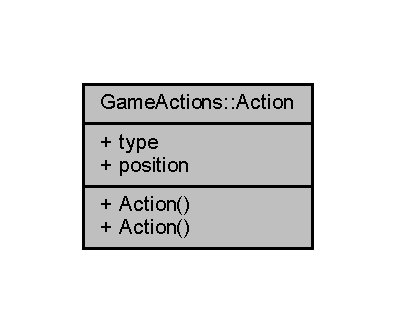
\includegraphics[width=190pt]{struct_game_actions_1_1_action__coll__graph}
\end{center}
\end{figure}
\subsection*{Fonctions membres publiques}
\begin{DoxyCompactItemize}
\item 
\hypertarget{struct_game_actions_1_1_action_a4f99d636b15eb70c090574871bc6e5c6}{}\label{struct_game_actions_1_1_action_a4f99d636b15eb70c090574871bc6e5c6} 
{\bfseries Action} (Type type, sf\+::\+Vector2f position)
\end{DoxyCompactItemize}
\subsection*{Attributs publics}
\begin{DoxyCompactItemize}
\item 
\hypertarget{struct_game_actions_1_1_action_ac4b04fe7c91e9f47d55665d7272b4622}{}\label{struct_game_actions_1_1_action_ac4b04fe7c91e9f47d55665d7272b4622} 
Type {\bfseries type}
\item 
\hypertarget{struct_game_actions_1_1_action_ac6834c74b5e0b5db797e2226da4dc83f}{}\label{struct_game_actions_1_1_action_ac6834c74b5e0b5db797e2226da4dc83f} 
sf\+::\+Vector2f {\bfseries position}
\end{DoxyCompactItemize}


\subsection{Description détaillée}


Définition à la ligne 64 du fichier Network\+Protocol.\+h.



La documentation de cette structure a été générée à partir du fichier suivant \+:\begin{DoxyCompactItemize}
\item 
Network\+Protocol.\+h\end{DoxyCompactItemize}

\hypertarget{class_aircraft}{}\section{Référence de la classe Aircraft}
\label{class_aircraft}\index{Aircraft@{Aircraft}}


Graphe d\textquotesingle{}héritage de Aircraft\+:\nopagebreak
\begin{figure}[H]
\begin{center}
\leavevmode
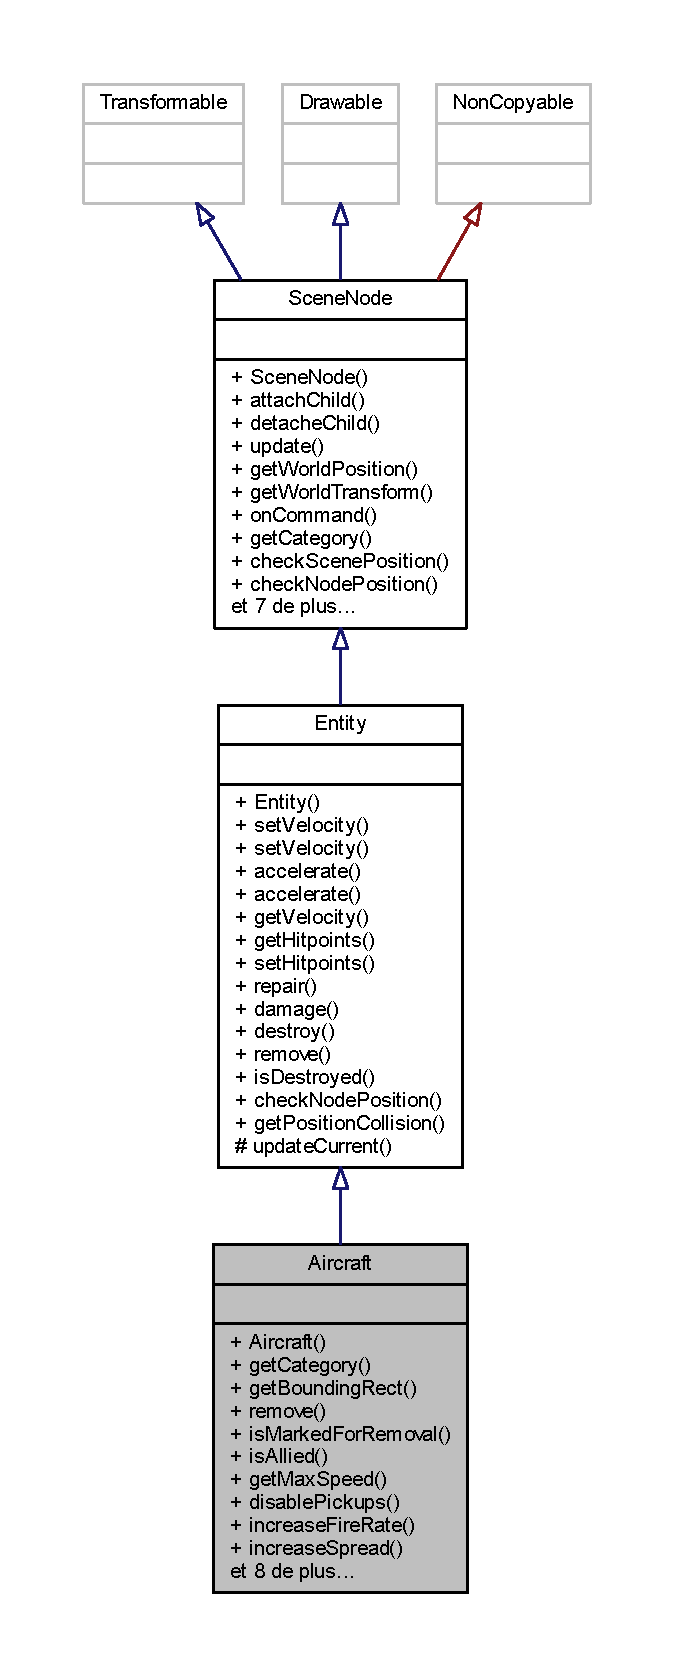
\includegraphics[width=350pt]{class_aircraft__inherit__graph}
\end{center}
\end{figure}


Graphe de collaboration de Aircraft\+:\nopagebreak
\begin{figure}[H]
\begin{center}
\leavevmode
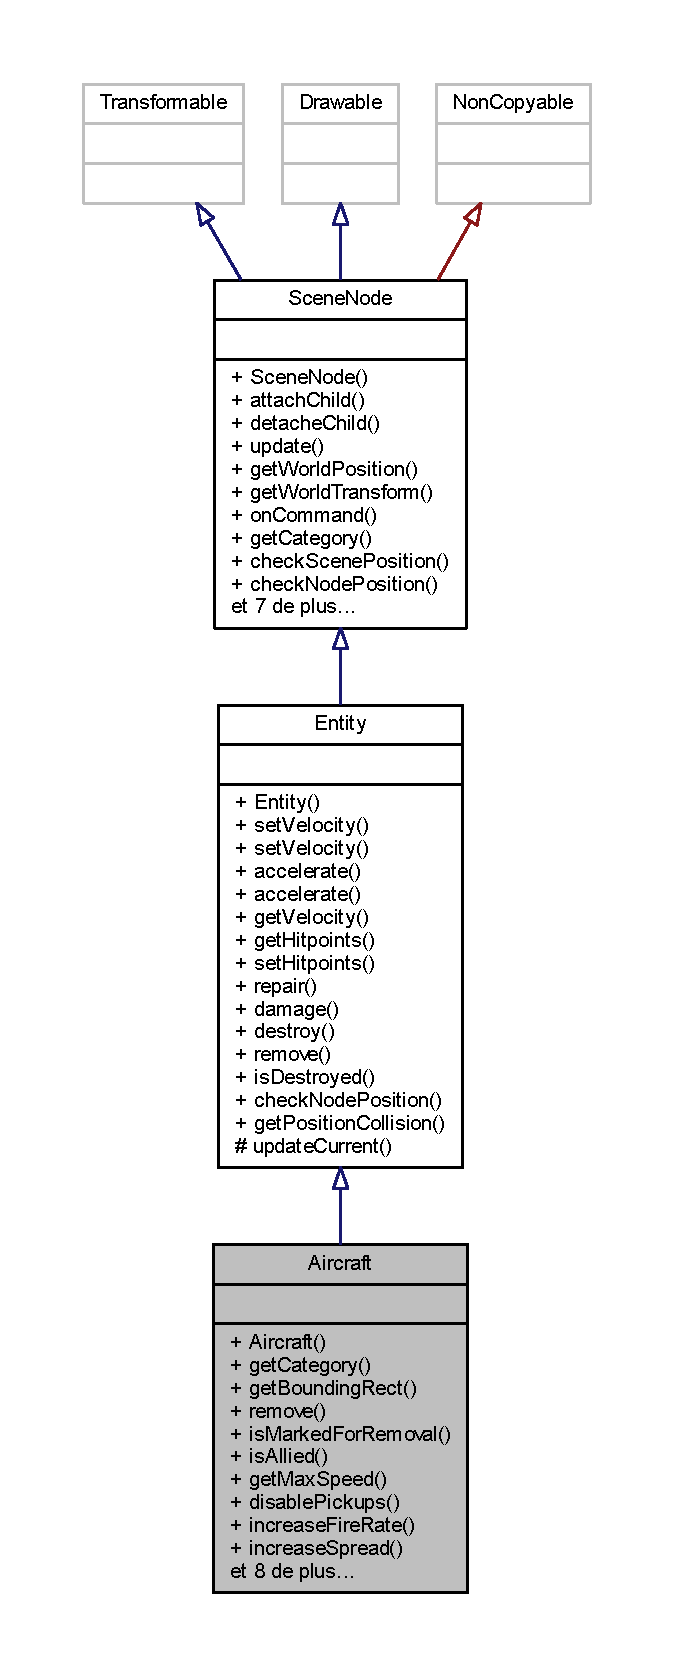
\includegraphics[width=350pt]{class_aircraft__coll__graph}
\end{center}
\end{figure}
\subsection*{Types publics}
\begin{DoxyCompactItemize}
\item 
enum {\bfseries Type} \{ {\bfseries Eagle}, 
{\bfseries Raptor}
 \}\hypertarget{class_aircraft_a7dae28542933e088032b753600046acd}{}\label{class_aircraft_a7dae28542933e088032b753600046acd}

\end{DoxyCompactItemize}
\subsection*{Fonctions membres publiques}
\begin{DoxyCompactItemize}
\item 
{\bfseries Aircraft} (Type type, const \hyperlink{class_resource_holder}{Texture\+Holder} \&textures)\hypertarget{class_aircraft_ae42f913aa28db8c4657e515a583af1d2}{}\label{class_aircraft_ae42f913aa28db8c4657e515a583af1d2}

\item 
virtual unsigned int {\bfseries get\+Category} () const \hypertarget{class_aircraft_aa6e117ff8572e1cb41842ecda2e9f23d}{}\label{class_aircraft_aa6e117ff8572e1cb41842ecda2e9f23d}

\end{DoxyCompactItemize}


La documentation de cette classe a été générée à partir des fichiers suivants \+:\begin{DoxyCompactItemize}
\item 
C\+:/\+Users/\+F\+R\+E\+D/\+Documents/\+F\+R\+E\+D/\+Programmation\+\_\+jeux/\+Projet\+\_\+\+S\+F\+M\+L/\+Projet2/include/Aircraft.\+h\item 
C\+:/\+Users/\+F\+R\+E\+D/\+Documents/\+F\+R\+E\+D/\+Programmation\+\_\+jeux/\+Projet\+\_\+\+S\+F\+M\+L/\+Projet2/src/Aircraft.\+cpp\end{DoxyCompactItemize}

\hypertarget{struct_aircraft_data}{}\section{Référence de la structure Aircraft\+Data}
\label{struct_aircraft_data}\index{Aircraft\+Data@{Aircraft\+Data}}


Graphe de collaboration de Aircraft\+Data\+:\nopagebreak
\begin{figure}[H]
\begin{center}
\leavevmode
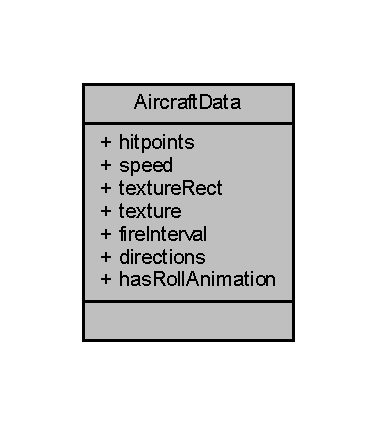
\includegraphics[width=181pt]{struct_aircraft_data__coll__graph}
\end{center}
\end{figure}
\subsection*{Attributs publics}
\begin{DoxyCompactItemize}
\item 
\hypertarget{struct_aircraft_data_ad2e89a12ab581641e79e97698c4bb751}{}\label{struct_aircraft_data_ad2e89a12ab581641e79e97698c4bb751} 
int {\bfseries hitpoints}
\item 
\hypertarget{struct_aircraft_data_a2edc576e968bfb7564f126010f85ca98}{}\label{struct_aircraft_data_a2edc576e968bfb7564f126010f85ca98} 
float {\bfseries speed}
\item 
\hypertarget{struct_aircraft_data_a8d6ac75aa2570404ee6b13c5d2128996}{}\label{struct_aircraft_data_a8d6ac75aa2570404ee6b13c5d2128996} 
sf\+::\+Int\+Rect {\bfseries texture\+Rect}
\item 
\hypertarget{struct_aircraft_data_a9c7f1508f44e99fd9376a2a8822f84a9}{}\label{struct_aircraft_data_a9c7f1508f44e99fd9376a2a8822f84a9} 
Textures\+::\+ID {\bfseries texture}
\item 
\hypertarget{struct_aircraft_data_a91ccdace300d5621ce8559b49fcb2efb}{}\label{struct_aircraft_data_a91ccdace300d5621ce8559b49fcb2efb} 
sf\+::\+Time {\bfseries fire\+Interval}
\item 
\hypertarget{struct_aircraft_data_a780a62ab0fb00cb4a01a5c539dcd06c3}{}\label{struct_aircraft_data_a780a62ab0fb00cb4a01a5c539dcd06c3} 
std\+::vector$<$ \hyperlink{struct_direction}{Direction} $>$ {\bfseries directions}
\item 
\hypertarget{struct_aircraft_data_aa9a2b05b21a194b31ff09b3604b56e39}{}\label{struct_aircraft_data_aa9a2b05b21a194b31ff09b3604b56e39} 
bool {\bfseries has\+Roll\+Animation}
\end{DoxyCompactItemize}


\subsection{Description détaillée}


Définition à la ligne 27 du fichier Data\+Tables.\+h.



La documentation de cette structure a été générée à partir du fichier suivant \+:\begin{DoxyCompactItemize}
\item 
Data\+Tables.\+h\end{DoxyCompactItemize}

\hypertarget{struct_aircraft_fire_trigger}{}\section{Référence de la structure Aircraft\+Fire\+Trigger}
\label{struct_aircraft_fire_trigger}\index{Aircraft\+Fire\+Trigger@{Aircraft\+Fire\+Trigger}}


Graphe de collaboration de Aircraft\+Fire\+Trigger\+:\nopagebreak
\begin{figure}[H]
\begin{center}
\leavevmode
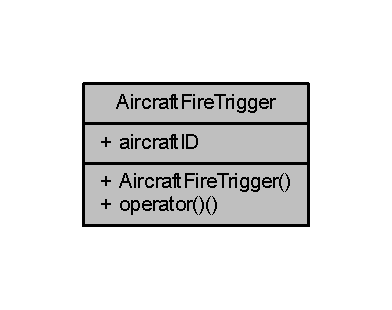
\includegraphics[width=188pt]{struct_aircraft_fire_trigger__coll__graph}
\end{center}
\end{figure}
\subsection*{Fonctions membres publiques}
\begin{DoxyCompactItemize}
\item 
\hypertarget{struct_aircraft_fire_trigger_a98857d290c7cedcfae7dd416d0c1ce6a}{}\label{struct_aircraft_fire_trigger_a98857d290c7cedcfae7dd416d0c1ce6a} 
{\bfseries Aircraft\+Fire\+Trigger} (int identifier)
\item 
\hypertarget{struct_aircraft_fire_trigger_ae155e735c722f7c821af34939d789628}{}\label{struct_aircraft_fire_trigger_ae155e735c722f7c821af34939d789628} 
void {\bfseries operator()} (\hyperlink{class_aircraft}{Aircraft} \&aircraft, sf\+::\+Time) const
\end{DoxyCompactItemize}
\subsection*{Attributs publics}
\begin{DoxyCompactItemize}
\item 
\hypertarget{struct_aircraft_fire_trigger_a57481c8c8d112cfe7fc689879f768bb3}{}\label{struct_aircraft_fire_trigger_a57481c8c8d112cfe7fc689879f768bb3} 
int {\bfseries aircraft\+ID}
\end{DoxyCompactItemize}


\subsection{Description détaillée}


Définition à la ligne 37 du fichier Player.\+cpp.



La documentation de cette structure a été générée à partir du fichier suivant \+:\begin{DoxyCompactItemize}
\item 
Player.\+cpp\end{DoxyCompactItemize}

\hypertarget{struct_aircraft_missile_trigger}{}\section{Référence de la structure Aircraft\+Missile\+Trigger}
\label{struct_aircraft_missile_trigger}\index{Aircraft\+Missile\+Trigger@{Aircraft\+Missile\+Trigger}}


Graphe de collaboration de Aircraft\+Missile\+Trigger\+:\nopagebreak
\begin{figure}[H]
\begin{center}
\leavevmode
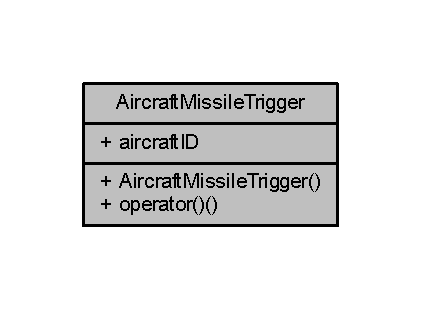
\includegraphics[width=202pt]{struct_aircraft_missile_trigger__coll__graph}
\end{center}
\end{figure}
\subsection*{Fonctions membres publiques}
\begin{DoxyCompactItemize}
\item 
\hypertarget{struct_aircraft_missile_trigger_a05b8d18e37581dc415b49b51d0ad2a11}{}\label{struct_aircraft_missile_trigger_a05b8d18e37581dc415b49b51d0ad2a11} 
{\bfseries Aircraft\+Missile\+Trigger} (int identifier)
\item 
\hypertarget{struct_aircraft_missile_trigger_a3e59059be448c10457d9b910312429f6}{}\label{struct_aircraft_missile_trigger_a3e59059be448c10457d9b910312429f6} 
void {\bfseries operator()} (\hyperlink{class_aircraft}{Aircraft} \&aircraft, sf\+::\+Time) const
\end{DoxyCompactItemize}
\subsection*{Attributs publics}
\begin{DoxyCompactItemize}
\item 
\hypertarget{struct_aircraft_missile_trigger_a27559c46b1b2fc265af9c216ffc1379f}{}\label{struct_aircraft_missile_trigger_a27559c46b1b2fc265af9c216ffc1379f} 
int {\bfseries aircraft\+ID}
\end{DoxyCompactItemize}


\subsection{Description détaillée}


Définition à la ligne 53 du fichier Player.\+cpp.



La documentation de cette structure a été générée à partir du fichier suivant \+:\begin{DoxyCompactItemize}
\item 
Player.\+cpp\end{DoxyCompactItemize}

\hypertarget{struct_aircraft_mover}{}\section{Référence de la structure Aircraft\+Mover}
\label{struct_aircraft_mover}\index{Aircraft\+Mover@{Aircraft\+Mover}}


Graphe de collaboration de Aircraft\+Mover\+:\nopagebreak
\begin{figure}[H]
\begin{center}
\leavevmode
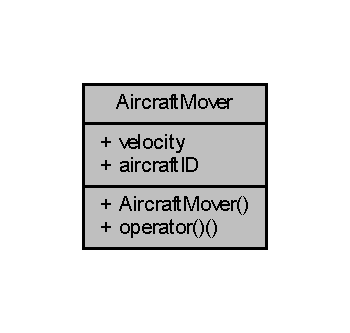
\includegraphics[width=168pt]{struct_aircraft_mover__coll__graph}
\end{center}
\end{figure}
\subsection*{Fonctions membres publiques}
\begin{DoxyCompactItemize}
\item 
{\bfseries Aircraft\+Mover} (float vx, float vy)\hypertarget{struct_aircraft_mover_a663cf13bc8568988fb45195efbea2a3b}{}\label{struct_aircraft_mover_a663cf13bc8568988fb45195efbea2a3b}

\item 
void {\bfseries operator()} (\hyperlink{class_aircraft}{Aircraft} \&aircraft, sf\+::\+Time) const \hypertarget{struct_aircraft_mover_a323a3dfc2bd9544018a98ce20baeea05}{}\label{struct_aircraft_mover_a323a3dfc2bd9544018a98ce20baeea05}

\end{DoxyCompactItemize}
\subsection*{Attributs publics}
\begin{DoxyCompactItemize}
\item 
sf\+::\+Vector2f {\bfseries velocity}\hypertarget{struct_aircraft_mover_a8403de0c4c7e057e7a47c6d38f621468}{}\label{struct_aircraft_mover_a8403de0c4c7e057e7a47c6d38f621468}

\end{DoxyCompactItemize}


La documentation de cette structure a été générée à partir du fichier suivant \+:\begin{DoxyCompactItemize}
\item 
C\+:/\+Users/\+F\+R\+E\+D/\+Documents/\+F\+R\+E\+D/\+Programmation\+\_\+jeux/\+Projet\+\_\+\+S\+F\+M\+L/\+Projet2/src/Player.\+cpp\end{DoxyCompactItemize}

\hypertarget{class_animation}{}\section{Référence de la classe Animation}
\label{class_animation}\index{Animation@{Animation}}


Graphe d\textquotesingle{}héritage de Animation\+:\nopagebreak
\begin{figure}[H]
\begin{center}
\leavevmode
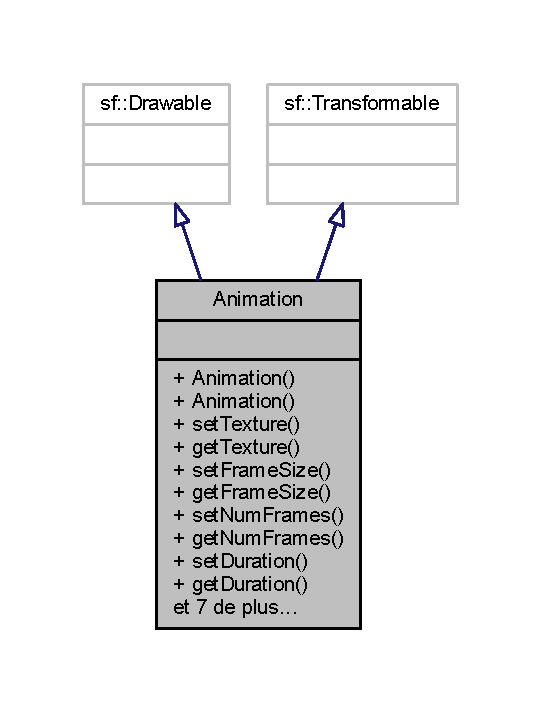
\includegraphics[width=260pt]{class_animation__inherit__graph}
\end{center}
\end{figure}


Graphe de collaboration de Animation\+:\nopagebreak
\begin{figure}[H]
\begin{center}
\leavevmode
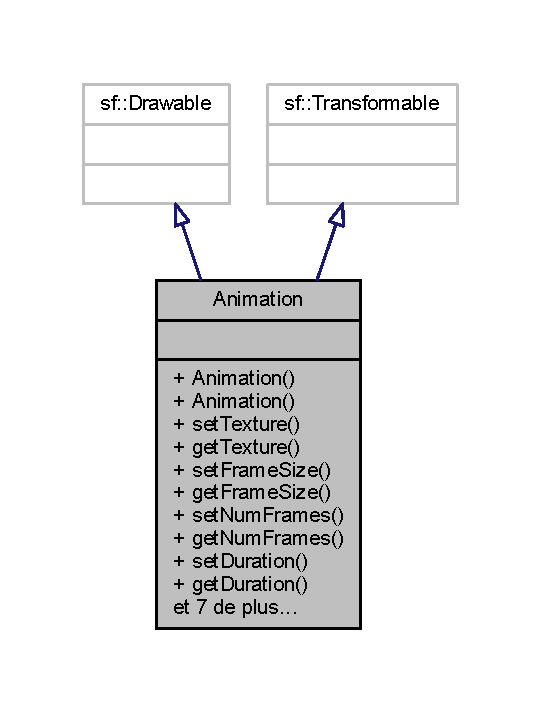
\includegraphics[width=260pt]{class_animation__coll__graph}
\end{center}
\end{figure}
\subsection*{Fonctions membres publiques}
\begin{DoxyCompactItemize}
\item 
\hypertarget{class_animation_a8f15adab6f0f4f37d0081c3902264334}{}\label{class_animation_a8f15adab6f0f4f37d0081c3902264334} 
{\bfseries Animation} (const sf\+::\+Texture \&texture)
\item 
\hypertarget{class_animation_a3d59fba435978a6531529041d355324b}{}\label{class_animation_a3d59fba435978a6531529041d355324b} 
void {\bfseries set\+Texture} (const sf\+::\+Texture \&texture)
\item 
\hypertarget{class_animation_aceb713113fea1038752e2d0018d0e304}{}\label{class_animation_aceb713113fea1038752e2d0018d0e304} 
const sf\+::\+Texture $\ast$ {\bfseries get\+Texture} () const
\item 
\hypertarget{class_animation_ad36304e4187bba21075bed5d57eb0025}{}\label{class_animation_ad36304e4187bba21075bed5d57eb0025} 
void {\bfseries set\+Frame\+Size} (sf\+::\+Vector2i m\+Frame\+Size)
\item 
\hypertarget{class_animation_ac94ce8b9abad85d686aec3ec8d05cd9f}{}\label{class_animation_ac94ce8b9abad85d686aec3ec8d05cd9f} 
sf\+::\+Vector2i {\bfseries get\+Frame\+Size} () const
\item 
\hypertarget{class_animation_aa056c5b431eb078bc7d36eacb12b299c}{}\label{class_animation_aa056c5b431eb078bc7d36eacb12b299c} 
void {\bfseries set\+Num\+Frames} (std\+::size\+\_\+t num\+Frames)
\item 
\hypertarget{class_animation_a9248e3726c272391ffaf1331bb72c3bf}{}\label{class_animation_a9248e3726c272391ffaf1331bb72c3bf} 
std\+::size\+\_\+t {\bfseries get\+Num\+Frames} () const
\item 
\hypertarget{class_animation_a168c112e11c1fe0040885cea8127dd83}{}\label{class_animation_a168c112e11c1fe0040885cea8127dd83} 
void {\bfseries set\+Duration} (sf\+::\+Time duration)
\item 
\hypertarget{class_animation_af8f00863383094851acb06d83f7a85e9}{}\label{class_animation_af8f00863383094851acb06d83f7a85e9} 
sf\+::\+Time {\bfseries get\+Duration} () const
\item 
\hypertarget{class_animation_ac6e19fdb858aab0b2b2f7e37d6976438}{}\label{class_animation_ac6e19fdb858aab0b2b2f7e37d6976438} 
void {\bfseries set\+Repeating} (bool flag)
\item 
\hypertarget{class_animation_aedcd2695ee980a41ff1fa65e0091f6a4}{}\label{class_animation_aedcd2695ee980a41ff1fa65e0091f6a4} 
bool {\bfseries is\+Repeating} () const
\item 
\hypertarget{class_animation_a17f07570ce8e26928fd1d99cfd9c63f0}{}\label{class_animation_a17f07570ce8e26928fd1d99cfd9c63f0} 
void {\bfseries restart} ()
\item 
\hypertarget{class_animation_a52f7a8449004b0248a3b7f8de9759cd0}{}\label{class_animation_a52f7a8449004b0248a3b7f8de9759cd0} 
bool {\bfseries is\+Finished} () const
\item 
\hypertarget{class_animation_a677e525e6b1f187fd6719bc511253a2b}{}\label{class_animation_a677e525e6b1f187fd6719bc511253a2b} 
sf\+::\+Float\+Rect {\bfseries get\+Local\+Bounds} () const
\item 
\hypertarget{class_animation_ad829ff72f859c44ea80b65aad5e7e5ae}{}\label{class_animation_ad829ff72f859c44ea80b65aad5e7e5ae} 
sf\+::\+Float\+Rect {\bfseries get\+Global\+Bounds} () const
\item 
\hypertarget{class_animation_a250fabaf23dab62bd373daac39aa25d3}{}\label{class_animation_a250fabaf23dab62bd373daac39aa25d3} 
void {\bfseries update} (sf\+::\+Time dt)
\end{DoxyCompactItemize}


\subsection{Description détaillée}


Définition à la ligne 8 du fichier Animation.\+h.



La documentation de cette classe a été générée à partir des fichiers suivants \+:\begin{DoxyCompactItemize}
\item 
Animation.\+h\item 
Animation.\+cpp\end{DoxyCompactItemize}

\hypertarget{class_application}{}\section{Référence de la classe Application}
\label{class_application}\index{Application@{Application}}


Graphe de collaboration de Application\+:\nopagebreak
\begin{figure}[H]
\begin{center}
\leavevmode
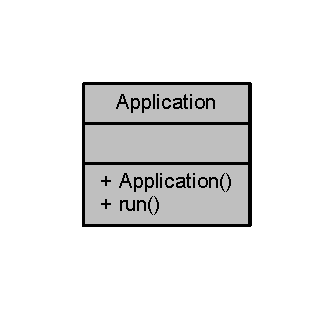
\includegraphics[width=160pt]{class_application__coll__graph}
\end{center}
\end{figure}
\subsection*{Fonctions membres publiques}
\begin{DoxyCompactItemize}
\item 
void {\bfseries run} ()\hypertarget{class_application_a68965449404743bf1add056784d6cf81}{}\label{class_application_a68965449404743bf1add056784d6cf81}

\end{DoxyCompactItemize}


La documentation de cette classe a été générée à partir des fichiers suivants \+:\begin{DoxyCompactItemize}
\item 
C\+:/\+Users/\+F\+R\+E\+D/\+Documents/\+F\+R\+E\+D/\+Programmation\+\_\+jeux/\+Projet\+\_\+\+S\+F\+M\+L/\+Projet2/include/Application.\+h\item 
C\+:/\+Users/\+F\+R\+E\+D/\+Documents/\+F\+R\+E\+D/\+Programmation\+\_\+jeux/\+Projet\+\_\+\+S\+F\+M\+L/\+Projet2/src/Application.\+cpp\end{DoxyCompactItemize}

\hypertarget{class_bloom_effect}{}\section{Référence de la classe Bloom\+Effect}
\label{class_bloom_effect}\index{Bloom\+Effect@{Bloom\+Effect}}


Graphe d\textquotesingle{}héritage de Bloom\+Effect\+:\nopagebreak
\begin{figure}[H]
\begin{center}
\leavevmode
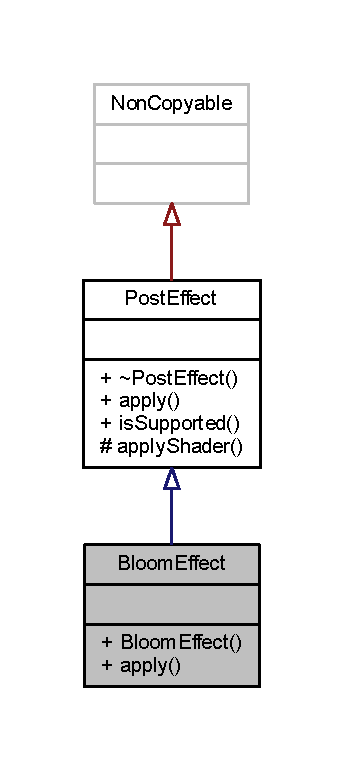
\includegraphics[width=165pt]{class_bloom_effect__inherit__graph}
\end{center}
\end{figure}


Graphe de collaboration de Bloom\+Effect\+:\nopagebreak
\begin{figure}[H]
\begin{center}
\leavevmode
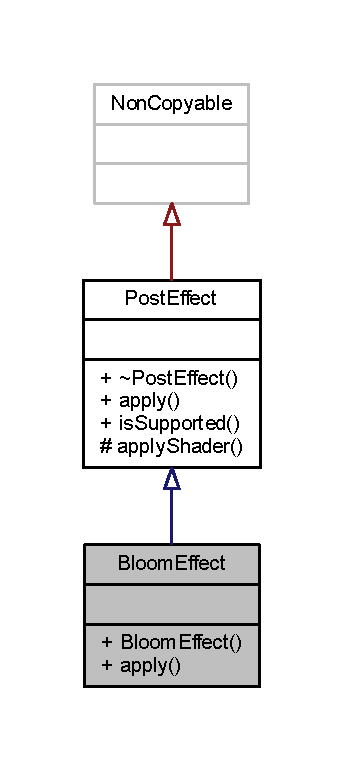
\includegraphics[width=165pt]{class_bloom_effect__coll__graph}
\end{center}
\end{figure}
\subsection*{Fonctions membres publiques}
\begin{DoxyCompactItemize}
\item 
\hypertarget{class_bloom_effect_add417d9fc98d72bf26bcab5e098de8c3}{}\label{class_bloom_effect_add417d9fc98d72bf26bcab5e098de8c3} 
virtual void {\bfseries apply} (const sf\+::\+Render\+Texture \&input, sf\+::\+Render\+Target \&output)
\end{DoxyCompactItemize}
\subsection*{Membres hérités additionnels}


\subsection{Description détaillée}


Définition à la ligne 14 du fichier Bloom\+Effect.\+h.



La documentation de cette classe a été générée à partir des fichiers suivants \+:\begin{DoxyCompactItemize}
\item 
Bloom\+Effect.\+h\item 
Bloom\+Effect.\+cpp\end{DoxyCompactItemize}

\hypertarget{class_g_u_i_1_1_button}{}\section{Référence de la classe G\+UI\+:\+:Button}
\label{class_g_u_i_1_1_button}\index{G\+U\+I\+::\+Button@{G\+U\+I\+::\+Button}}


Graphe d\textquotesingle{}héritage de G\+UI\+:\+:Button\+:\nopagebreak
\begin{figure}[H]
\begin{center}
\leavevmode
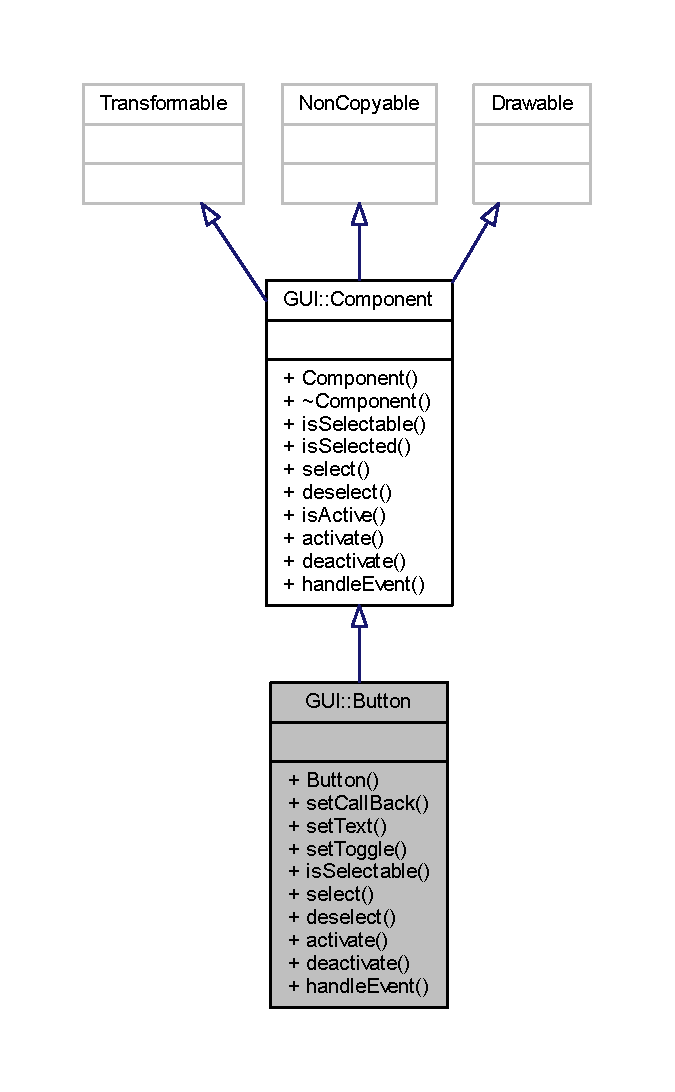
\includegraphics[width=324pt]{class_g_u_i_1_1_button__inherit__graph}
\end{center}
\end{figure}


Graphe de collaboration de G\+UI\+:\+:Button\+:\nopagebreak
\begin{figure}[H]
\begin{center}
\leavevmode
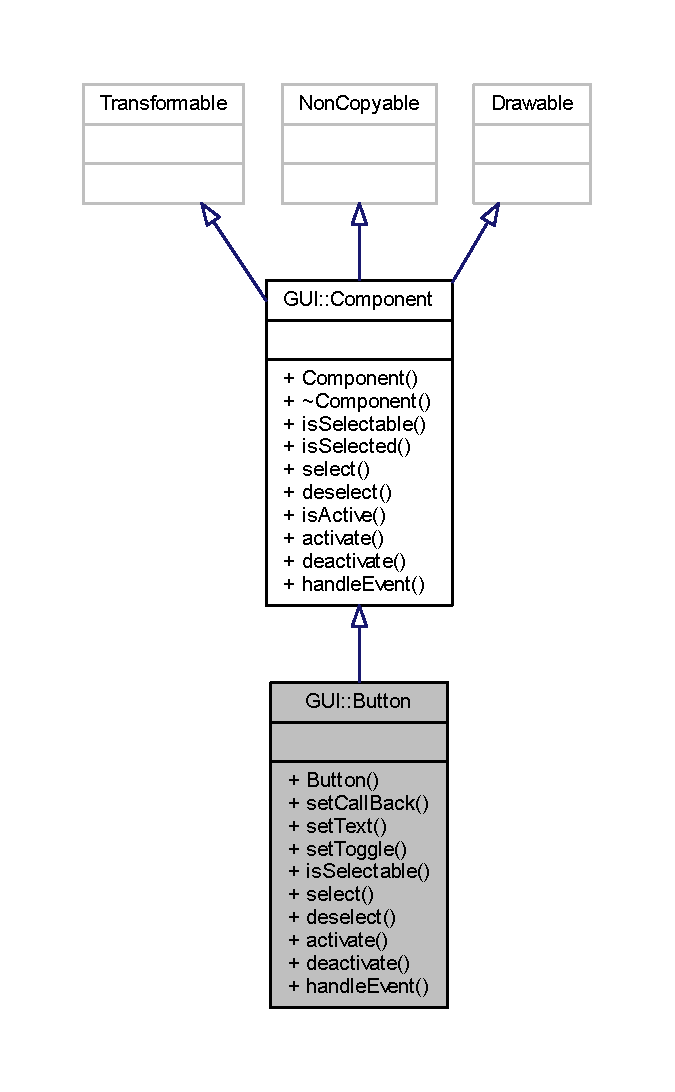
\includegraphics[width=324pt]{class_g_u_i_1_1_button__coll__graph}
\end{center}
\end{figure}
\subsection*{Types publics}
\begin{DoxyCompactItemize}
\item 
\hypertarget{class_g_u_i_1_1_button_a405149f049ffc8144e11e73fec3bae96}{}\label{class_g_u_i_1_1_button_a405149f049ffc8144e11e73fec3bae96} 
enum {\bfseries Type} \{ {\bfseries Normal}, 
{\bfseries Selected}, 
{\bfseries Pressed}, 
{\bfseries Button\+Count}
 \}
\item 
\hypertarget{class_g_u_i_1_1_button_a910df9f7797f35d65b43da4dd392f1de}{}\label{class_g_u_i_1_1_button_a910df9f7797f35d65b43da4dd392f1de} 
typedef std\+::shared\+\_\+ptr$<$ \hyperlink{class_g_u_i_1_1_button}{Button} $>$ {\bfseries Ptr}
\item 
\hypertarget{class_g_u_i_1_1_button_a7f3887a6bc45f72fec7dd56c639f563d}{}\label{class_g_u_i_1_1_button_a7f3887a6bc45f72fec7dd56c639f563d} 
typedef std\+::function$<$ void()$>$ {\bfseries Call\+Back}
\end{DoxyCompactItemize}
\subsection*{Fonctions membres publiques}
\begin{DoxyCompactItemize}
\item 
\hypertarget{class_g_u_i_1_1_button_a8e44cbb42ddc953245922e6b6981ab58}{}\label{class_g_u_i_1_1_button_a8e44cbb42ddc953245922e6b6981ab58} 
{\bfseries Button} (\hyperlink{struct_state_1_1_context}{State\+::\+Context} context)
\item 
\hypertarget{class_g_u_i_1_1_button_a31d184f24a264215a7d4eb53a216d6ea}{}\label{class_g_u_i_1_1_button_a31d184f24a264215a7d4eb53a216d6ea} 
void {\bfseries set\+Call\+Back} (Call\+Back call\+Back)
\item 
\hypertarget{class_g_u_i_1_1_button_a89e964d353192135d6a77aeff33bbc41}{}\label{class_g_u_i_1_1_button_a89e964d353192135d6a77aeff33bbc41} 
void {\bfseries set\+Text} (const std\+::string \&text)
\item 
\hypertarget{class_g_u_i_1_1_button_a8198052cf4fe5823c9f5513e778ca94d}{}\label{class_g_u_i_1_1_button_a8198052cf4fe5823c9f5513e778ca94d} 
void {\bfseries set\+Toggle} (bool flag)
\item 
\hypertarget{class_g_u_i_1_1_button_a3a8cf4907161a7cc75a9353dd48c4f12}{}\label{class_g_u_i_1_1_button_a3a8cf4907161a7cc75a9353dd48c4f12} 
virtual bool {\bfseries is\+Selectable} () const
\item 
\hypertarget{class_g_u_i_1_1_button_a8f141129acb9c068ba6b8d19974d8291}{}\label{class_g_u_i_1_1_button_a8f141129acb9c068ba6b8d19974d8291} 
virtual void {\bfseries select} ()
\item 
\hypertarget{class_g_u_i_1_1_button_a6fd040a471dc3ae48ad59cacd93c7292}{}\label{class_g_u_i_1_1_button_a6fd040a471dc3ae48ad59cacd93c7292} 
virtual void {\bfseries deselect} ()
\item 
\hypertarget{class_g_u_i_1_1_button_ad711a129863e0301c52b896911996123}{}\label{class_g_u_i_1_1_button_ad711a129863e0301c52b896911996123} 
virtual void {\bfseries activate} ()
\item 
\hypertarget{class_g_u_i_1_1_button_ab0a1773817447712b17ab1ad6da767da}{}\label{class_g_u_i_1_1_button_ab0a1773817447712b17ab1ad6da767da} 
virtual void {\bfseries deactivate} ()
\item 
\hypertarget{class_g_u_i_1_1_button_a4d30e4caedd4c4373567ef452acd1fb1}{}\label{class_g_u_i_1_1_button_a4d30e4caedd4c4373567ef452acd1fb1} 
virtual void {\bfseries handle\+Event} (const sf\+::\+Event \&event)
\end{DoxyCompactItemize}


\subsection{Description détaillée}


Définition à la ligne 22 du fichier Button.\+h.



La documentation de cette classe a été générée à partir des fichiers suivants \+:\begin{DoxyCompactItemize}
\item 
Button.\+h\item 
Button.\+cpp\end{DoxyCompactItemize}

\hypertarget{struct_command}{}\section{Référence de la structure Command}
\label{struct_command}\index{Command@{Command}}


Graphe de collaboration de Command\+:\nopagebreak
\begin{figure}[H]
\begin{center}
\leavevmode
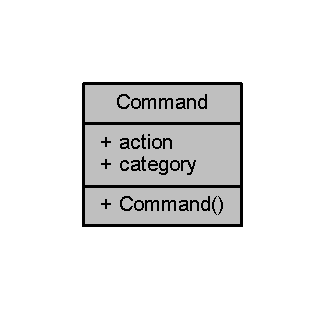
\includegraphics[width=156pt]{struct_command__coll__graph}
\end{center}
\end{figure}
\subsection*{Attributs publics}
\begin{DoxyCompactItemize}
\item 
\hypertarget{struct_command_a104fe6a9eb7bc8fc2f23acc67eb2b1d9}{}\label{struct_command_a104fe6a9eb7bc8fc2f23acc67eb2b1d9} 
std\+::function$<$ void(\hyperlink{class_scene_node}{Scene\+Node} \&, sf\+::\+Time)$>$ {\bfseries action}
\item 
\hypertarget{struct_command_a1529e898c9e6dd47b1826b5b1eac09fb}{}\label{struct_command_a1529e898c9e6dd47b1826b5b1eac09fb} 
unsigned int {\bfseries category}
\end{DoxyCompactItemize}


\subsection{Description détaillée}


Définition à la ligne 16 du fichier Command.\+h.



La documentation de cette structure a été générée à partir des fichiers suivants \+:\begin{DoxyCompactItemize}
\item 
Command.\+h\item 
Command.\+cpp\end{DoxyCompactItemize}

\hypertarget{class_command_queue}{}\section{Référence de la classe Command\+Queue}
\label{class_command_queue}\index{Command\+Queue@{Command\+Queue}}


Graphe de collaboration de Command\+Queue\+:\nopagebreak
\begin{figure}[H]
\begin{center}
\leavevmode
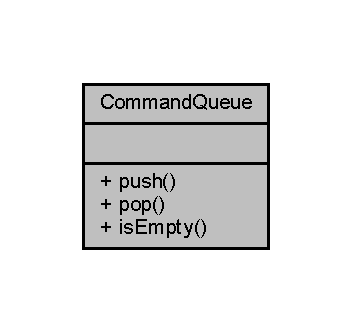
\includegraphics[width=169pt]{class_command_queue__coll__graph}
\end{center}
\end{figure}
\subsection*{Fonctions membres publiques}
\begin{DoxyCompactItemize}
\item 
void {\bfseries push} (const \hyperlink{struct_command}{Command} \&command)\hypertarget{class_command_queue_ad444e0d7af45d9e09b834f0cec1e1f43}{}\label{class_command_queue_ad444e0d7af45d9e09b834f0cec1e1f43}

\item 
\hyperlink{struct_command}{Command} {\bfseries pop} ()\hypertarget{class_command_queue_ac2dde510222b8df393b55978f4594194}{}\label{class_command_queue_ac2dde510222b8df393b55978f4594194}

\item 
bool {\bfseries is\+Empty} () const \hypertarget{class_command_queue_ad4f4731c185a293724a59aba9a5903d6}{}\label{class_command_queue_ad4f4731c185a293724a59aba9a5903d6}

\end{DoxyCompactItemize}


La documentation de cette classe a été générée à partir des fichiers suivants \+:\begin{DoxyCompactItemize}
\item 
C\+:/\+Users/\+F\+R\+E\+D/\+Documents/\+F\+R\+E\+D/\+Programmation\+\_\+jeux/\+Projet\+\_\+\+S\+F\+M\+L/\+Projet2/include/Command\+Queue.\+h\item 
C\+:/\+Users/\+F\+R\+E\+D/\+Documents/\+F\+R\+E\+D/\+Programmation\+\_\+jeux/\+Projet\+\_\+\+S\+F\+M\+L/\+Projet2/src/Command\+Queue.\+cpp\end{DoxyCompactItemize}

\hypertarget{class_g_u_i_1_1_component}{}\section{Référence de la classe G\+UI\+:\+:Component}
\label{class_g_u_i_1_1_component}\index{G\+U\+I\+::\+Component@{G\+U\+I\+::\+Component}}


Graphe d\textquotesingle{}héritage de G\+UI\+:\+:Component\+:\nopagebreak
\begin{figure}[H]
\begin{center}
\leavevmode
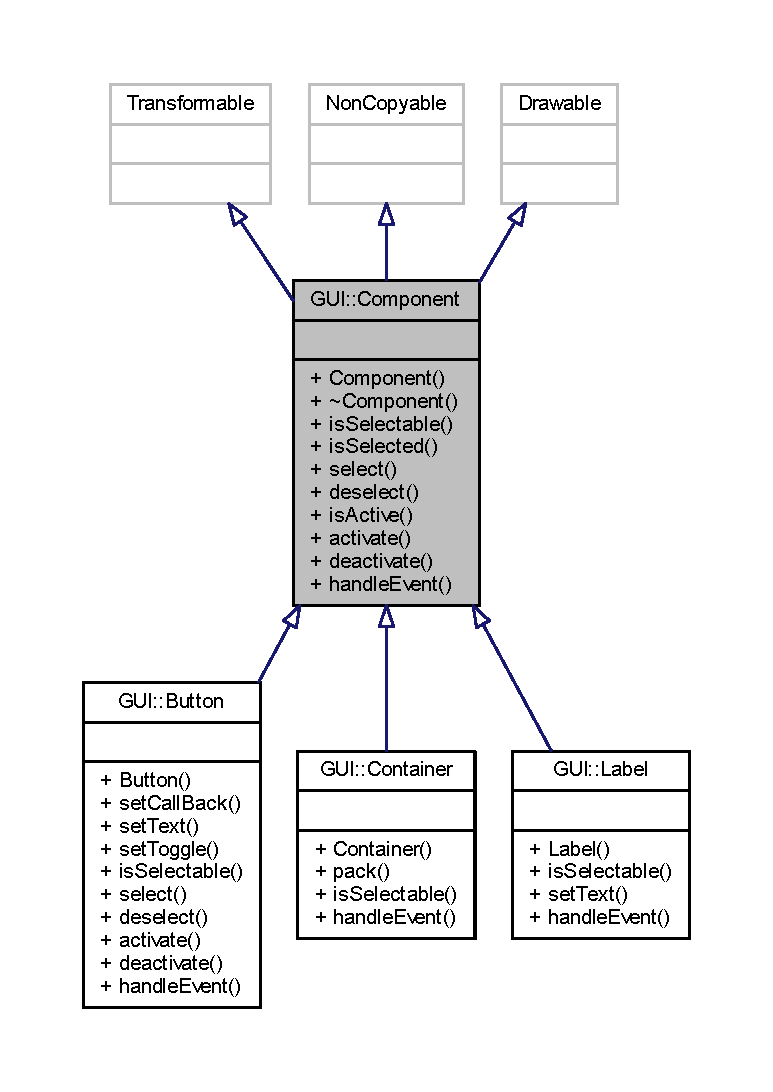
\includegraphics[width=350pt]{class_g_u_i_1_1_component__inherit__graph}
\end{center}
\end{figure}


Graphe de collaboration de G\+UI\+:\+:Component\+:\nopagebreak
\begin{figure}[H]
\begin{center}
\leavevmode
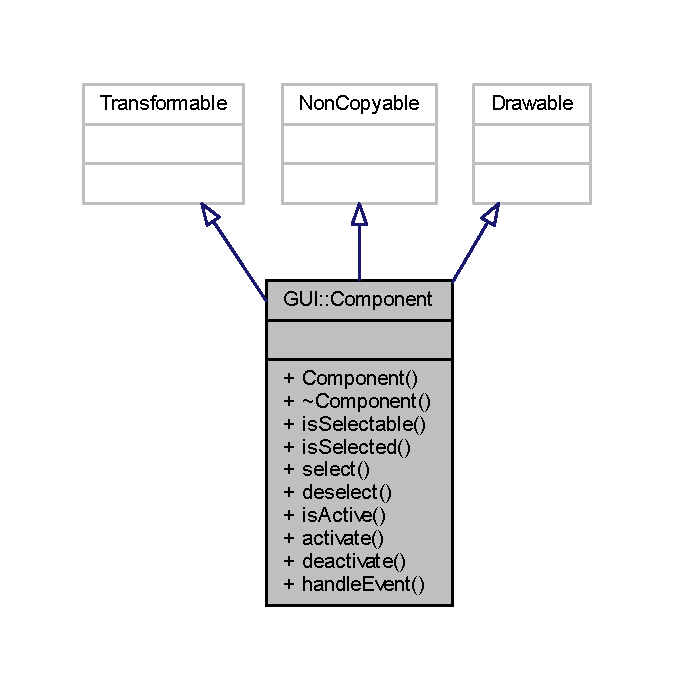
\includegraphics[width=324pt]{class_g_u_i_1_1_component__coll__graph}
\end{center}
\end{figure}
\subsection*{Types publics}
\begin{DoxyCompactItemize}
\item 
\hypertarget{class_g_u_i_1_1_component_aa51eb17541f4cbe71b60cf7e1e16f32b}{}\label{class_g_u_i_1_1_component_aa51eb17541f4cbe71b60cf7e1e16f32b} 
typedef std\+::shared\+\_\+ptr$<$ \hyperlink{class_g_u_i_1_1_component}{Component} $>$ {\bfseries Ptr}
\end{DoxyCompactItemize}
\subsection*{Fonctions membres publiques}
\begin{DoxyCompactItemize}
\item 
\hypertarget{class_g_u_i_1_1_component_a44d14506c9a1dbc839e05a6bf99c341b}{}\label{class_g_u_i_1_1_component_a44d14506c9a1dbc839e05a6bf99c341b} 
virtual bool {\bfseries is\+Selectable} () const =0
\item 
\hypertarget{class_g_u_i_1_1_component_a456e20a33a9ee778b0eda2641147724e}{}\label{class_g_u_i_1_1_component_a456e20a33a9ee778b0eda2641147724e} 
bool {\bfseries is\+Selected} () const
\item 
\hypertarget{class_g_u_i_1_1_component_ad0f7d6cc692edf2b0e426bfbd584be45}{}\label{class_g_u_i_1_1_component_ad0f7d6cc692edf2b0e426bfbd584be45} 
virtual void {\bfseries select} ()
\item 
\hypertarget{class_g_u_i_1_1_component_aa37424b238293bb308d357cf3b35c81f}{}\label{class_g_u_i_1_1_component_aa37424b238293bb308d357cf3b35c81f} 
virtual void {\bfseries deselect} ()
\item 
\hypertarget{class_g_u_i_1_1_component_a86d906696a080742900b8ead67a2ae3b}{}\label{class_g_u_i_1_1_component_a86d906696a080742900b8ead67a2ae3b} 
virtual bool {\bfseries is\+Active} () const
\item 
\hypertarget{class_g_u_i_1_1_component_a965823e0e62612a7e532eb8c0b98861d}{}\label{class_g_u_i_1_1_component_a965823e0e62612a7e532eb8c0b98861d} 
virtual void {\bfseries activate} ()
\item 
\hypertarget{class_g_u_i_1_1_component_a8964087afef859c015fb8188e619aa81}{}\label{class_g_u_i_1_1_component_a8964087afef859c015fb8188e619aa81} 
virtual void {\bfseries deactivate} ()
\item 
\hypertarget{class_g_u_i_1_1_component_aacf5e981e7b5726f5c7e9436455660ba}{}\label{class_g_u_i_1_1_component_aacf5e981e7b5726f5c7e9436455660ba} 
virtual void {\bfseries handle\+Event} (const sf\+::\+Event \&event)=0
\end{DoxyCompactItemize}


\subsection{Description détaillée}


Définition à la ligne 18 du fichier Component.\+h.



La documentation de cette classe a été générée à partir des fichiers suivants \+:\begin{DoxyCompactItemize}
\item 
Component.\+h\item 
Component.\+cpp\end{DoxyCompactItemize}

\hypertarget{class_g_u_i_1_1_container}{}\section{Référence de la classe G\+UI\+:\+:Container}
\label{class_g_u_i_1_1_container}\index{G\+U\+I\+::\+Container@{G\+U\+I\+::\+Container}}


Graphe d\textquotesingle{}héritage de G\+UI\+:\+:Container\+:\nopagebreak
\begin{figure}[H]
\begin{center}
\leavevmode
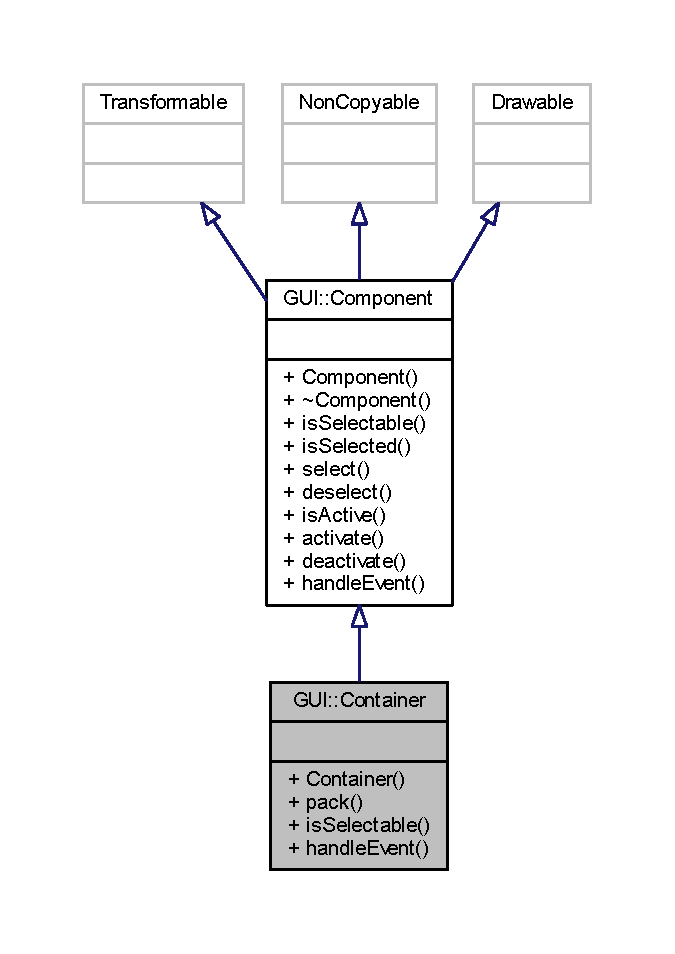
\includegraphics[width=324pt]{class_g_u_i_1_1_container__inherit__graph}
\end{center}
\end{figure}


Graphe de collaboration de G\+UI\+:\+:Container\+:\nopagebreak
\begin{figure}[H]
\begin{center}
\leavevmode
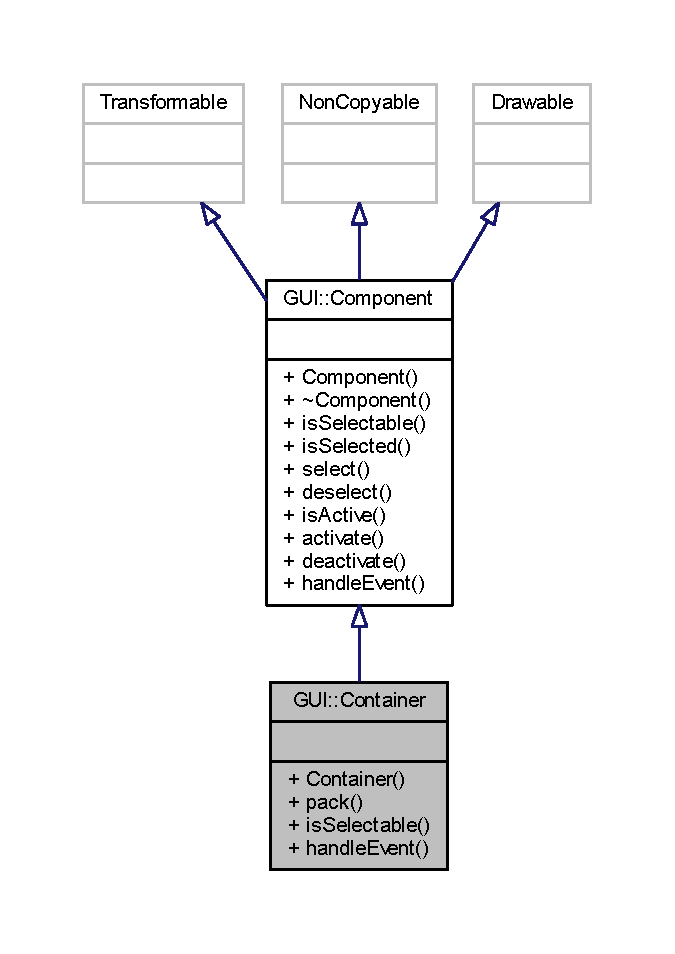
\includegraphics[width=324pt]{class_g_u_i_1_1_container__coll__graph}
\end{center}
\end{figure}
\subsection*{Types publics}
\begin{DoxyCompactItemize}
\item 
\hypertarget{class_g_u_i_1_1_container_aff900329cc0dbef99abdd1c95175823a}{}\label{class_g_u_i_1_1_container_aff900329cc0dbef99abdd1c95175823a} 
typedef std\+::shared\+\_\+ptr$<$ \hyperlink{class_g_u_i_1_1_container}{Container} $>$ {\bfseries Ptr}
\end{DoxyCompactItemize}
\subsection*{Fonctions membres publiques}
\begin{DoxyCompactItemize}
\item 
\hypertarget{class_g_u_i_1_1_container_a6f6217ae300a4f313a55f01f17baf5d6}{}\label{class_g_u_i_1_1_container_a6f6217ae300a4f313a55f01f17baf5d6} 
void {\bfseries pack} (Component\+::\+Ptr \hyperlink{class_g_u_i_1_1_component}{Component})
\item 
\hypertarget{class_g_u_i_1_1_container_a6a5c4b42556336e194a90c68a035174d}{}\label{class_g_u_i_1_1_container_a6a5c4b42556336e194a90c68a035174d} 
virtual bool {\bfseries is\+Selectable} () const
\item 
\hypertarget{class_g_u_i_1_1_container_af08db9d157a4e56f706493529901eb7f}{}\label{class_g_u_i_1_1_container_af08db9d157a4e56f706493529901eb7f} 
virtual void {\bfseries handle\+Event} (const sf\+::\+Event \&event)
\end{DoxyCompactItemize}


\subsection{Description détaillée}


Définition à la ligne 11 du fichier Container.\+h.



La documentation de cette classe a été générée à partir des fichiers suivants \+:\begin{DoxyCompactItemize}
\item 
Container.\+h\item 
Container.\+cpp\end{DoxyCompactItemize}

\hypertarget{struct_state_1_1_context}{}\section{Référence de la structure State\+:\+:Context}
\label{struct_state_1_1_context}\index{State\+::\+Context@{State\+::\+Context}}


Graphe de collaboration de State\+:\+:Context\+:\nopagebreak
\begin{figure}[H]
\begin{center}
\leavevmode
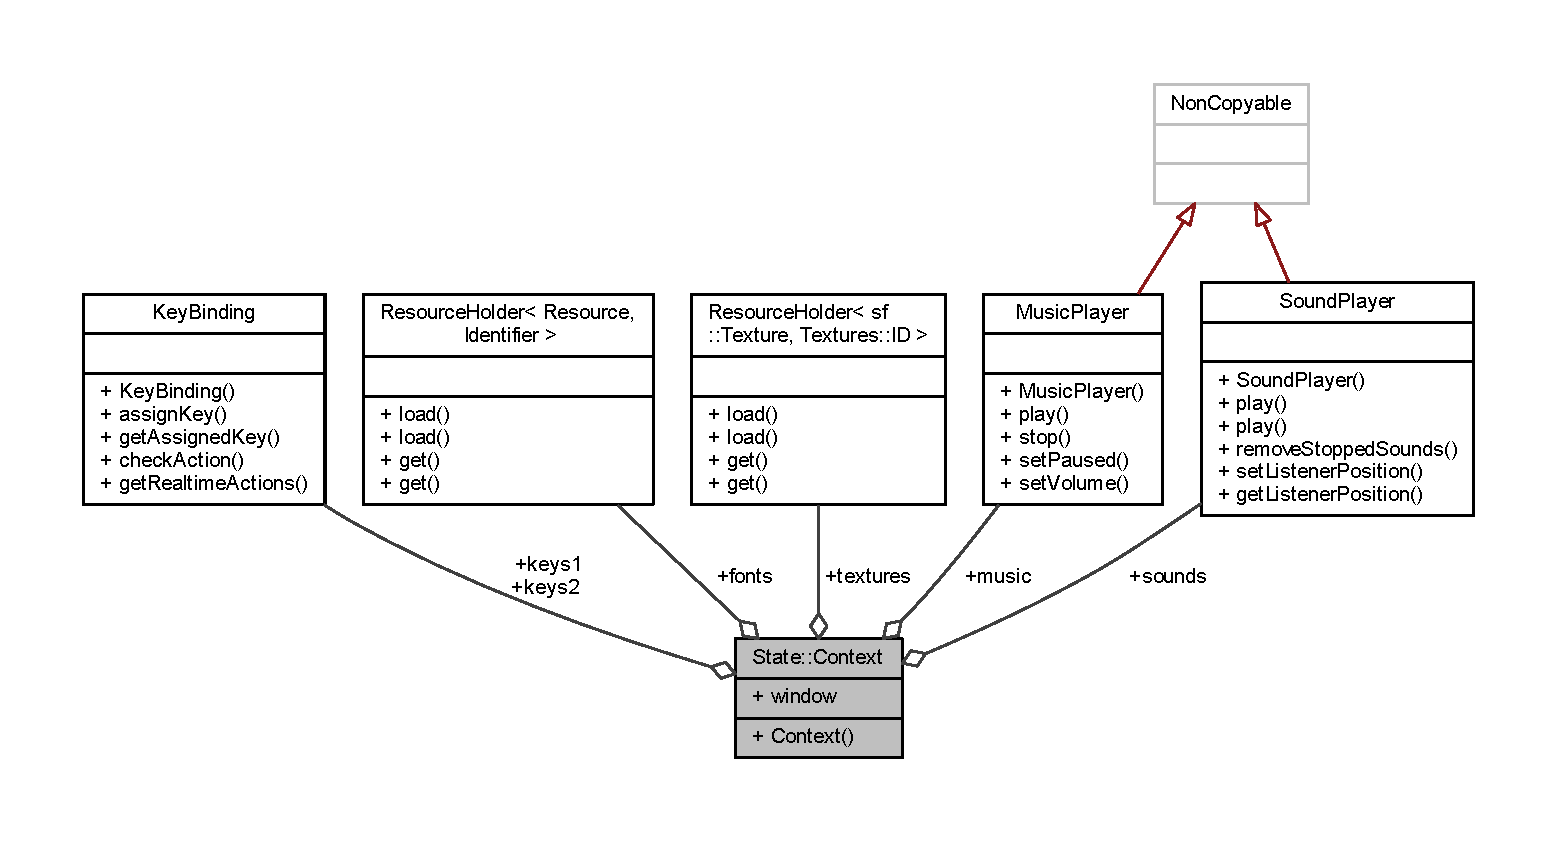
\includegraphics[width=350pt]{struct_state_1_1_context__coll__graph}
\end{center}
\end{figure}
\subsection*{Fonctions membres publiques}
\begin{DoxyCompactItemize}
\item 
{\bfseries Context} (sf\+::\+Render\+Window \&window, \hyperlink{class_resource_holder}{Texture\+Holder} \&textures, \hyperlink{class_resource_holder}{Font\+Holder} \&fonts, \hyperlink{class_player}{Player} \&player)\hypertarget{struct_state_1_1_context_ac8380f7873b3248c7cf32c604bbdda26}{}\label{struct_state_1_1_context_ac8380f7873b3248c7cf32c604bbdda26}

\end{DoxyCompactItemize}
\subsection*{Attributs publics}
\begin{DoxyCompactItemize}
\item 
sf\+::\+Render\+Window $\ast$ {\bfseries window}\hypertarget{struct_state_1_1_context_a30775e70e841c761a4e3cb7f0e195128}{}\label{struct_state_1_1_context_a30775e70e841c761a4e3cb7f0e195128}

\item 
\hyperlink{class_resource_holder}{Texture\+Holder} $\ast$ {\bfseries textures}\hypertarget{struct_state_1_1_context_a587123ee3b00e8c68c1d99ca6011a53d}{}\label{struct_state_1_1_context_a587123ee3b00e8c68c1d99ca6011a53d}

\item 
\hyperlink{class_resource_holder}{Font\+Holder} $\ast$ {\bfseries fonts}\hypertarget{struct_state_1_1_context_a8b4a94c250018312ccf2e58a33f0c77a}{}\label{struct_state_1_1_context_a8b4a94c250018312ccf2e58a33f0c77a}

\item 
\hyperlink{class_player}{Player} $\ast$ {\bfseries player}\hypertarget{struct_state_1_1_context_a1c98434687748acdebf78fd80a4767ad}{}\label{struct_state_1_1_context_a1c98434687748acdebf78fd80a4767ad}

\end{DoxyCompactItemize}


La documentation de cette structure a été générée à partir des fichiers suivants \+:\begin{DoxyCompactItemize}
\item 
C\+:/\+Users/\+F\+R\+E\+D/\+Documents/\+F\+R\+E\+D/\+Programmation\+\_\+jeux/\+Projet\+\_\+\+S\+F\+M\+L/\+Projet2/include/State.\+h\item 
C\+:/\+Users/\+F\+R\+E\+D/\+Documents/\+F\+R\+E\+D/\+Programmation\+\_\+jeux/\+Projet\+\_\+\+S\+F\+M\+L/\+Projet2/src/State.\+cpp\end{DoxyCompactItemize}

\hypertarget{struct_direction}{}\section{Référence de la structure Direction}
\label{struct_direction}\index{Direction@{Direction}}


Graphe de collaboration de Direction\+:\nopagebreak
\begin{figure}[H]
\begin{center}
\leavevmode
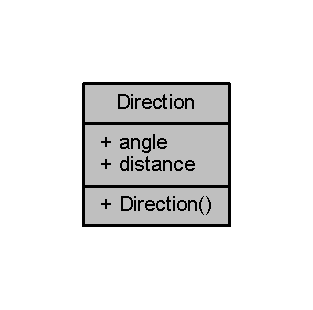
\includegraphics[width=150pt]{struct_direction__coll__graph}
\end{center}
\end{figure}
\subsection*{Fonctions membres publiques}
\begin{DoxyCompactItemize}
\item 
\hypertarget{struct_direction_ad8439f2ac8ed58d652d9f1c40e66c065}{}\label{struct_direction_ad8439f2ac8ed58d652d9f1c40e66c065} 
{\bfseries Direction} (float angle, float distance)
\end{DoxyCompactItemize}
\subsection*{Attributs publics}
\begin{DoxyCompactItemize}
\item 
\hypertarget{struct_direction_a8eaabd2d06c6274e92866814cfb6a2ea}{}\label{struct_direction_a8eaabd2d06c6274e92866814cfb6a2ea} 
float {\bfseries angle}
\item 
\hypertarget{struct_direction_a6cf81244bffe43d4b4d1bc8a3f63772a}{}\label{struct_direction_a6cf81244bffe43d4b4d1bc8a3f63772a} 
float {\bfseries distance}
\end{DoxyCompactItemize}


\subsection{Description détaillée}


Définition à la ligne 15 du fichier Data\+Tables.\+h.



La documentation de cette structure a été générée à partir du fichier suivant \+:\begin{DoxyCompactItemize}
\item 
Data\+Tables.\+h\end{DoxyCompactItemize}

\hypertarget{class_emitter_node}{}\section{Référence de la classe Emitter\+Node}
\label{class_emitter_node}\index{Emitter\+Node@{Emitter\+Node}}


Graphe d\textquotesingle{}héritage de Emitter\+Node\+:\nopagebreak
\begin{figure}[H]
\begin{center}
\leavevmode
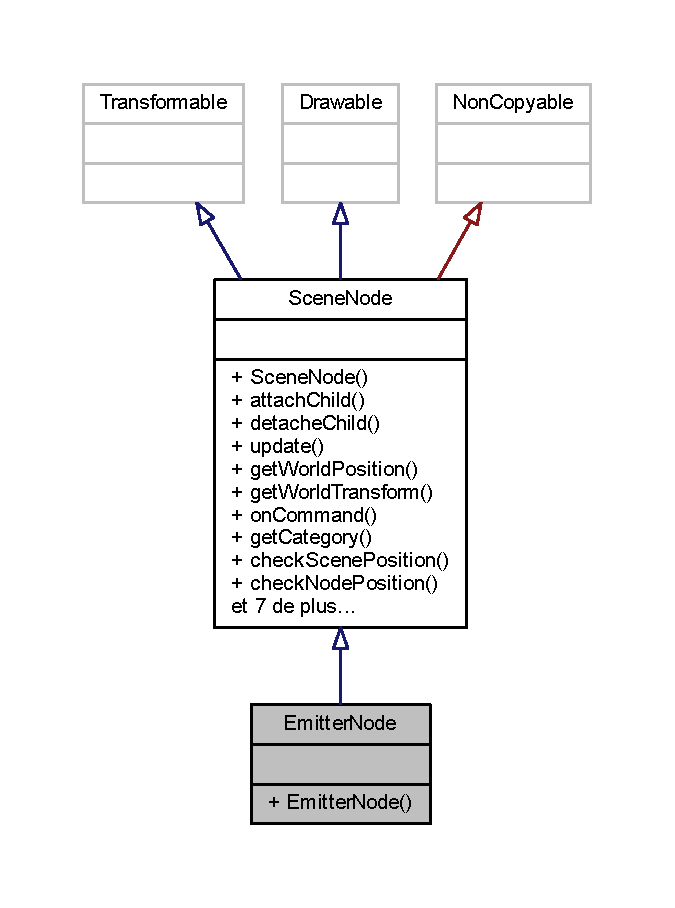
\includegraphics[width=324pt]{class_emitter_node__inherit__graph}
\end{center}
\end{figure}


Graphe de collaboration de Emitter\+Node\+:\nopagebreak
\begin{figure}[H]
\begin{center}
\leavevmode
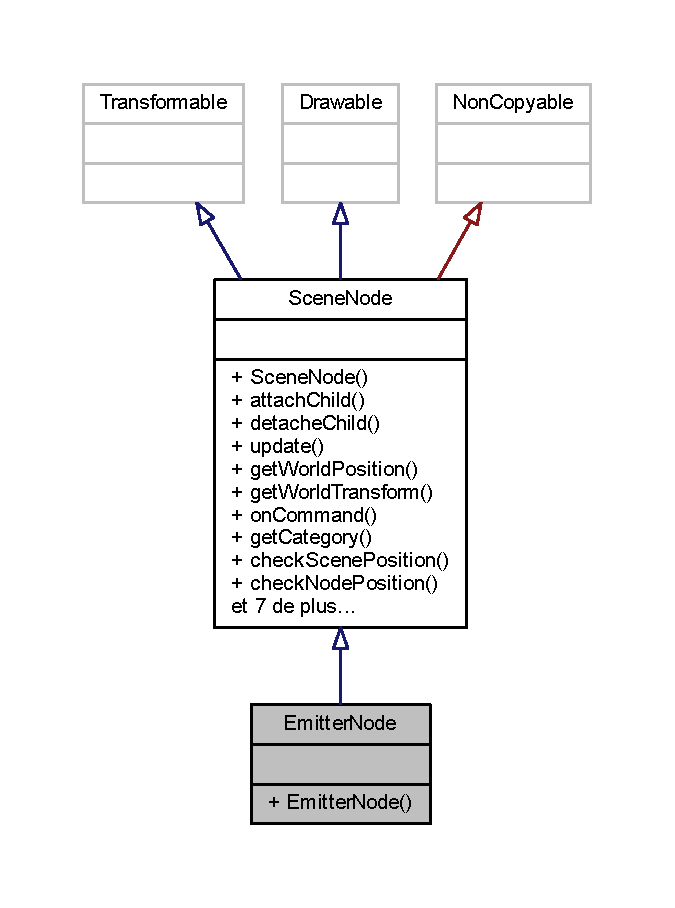
\includegraphics[width=324pt]{class_emitter_node__coll__graph}
\end{center}
\end{figure}
\subsection*{Fonctions membres publiques}
\begin{DoxyCompactItemize}
\item 
\hypertarget{class_emitter_node_a8a6ba67d44a62d87448fab0959e15646}{}\label{class_emitter_node_a8a6ba67d44a62d87448fab0959e15646} 
{\bfseries Emitter\+Node} (Particle\+::\+Type type)
\end{DoxyCompactItemize}
\subsection*{Membres hérités additionnels}


\subsection{Description détaillée}


Définition à la ligne 9 du fichier Emitter\+Node.\+h.



La documentation de cette classe a été générée à partir des fichiers suivants \+:\begin{DoxyCompactItemize}
\item 
Emitter\+Node.\+h\item 
Emitter\+Node.\+cpp\end{DoxyCompactItemize}

\hypertarget{class_entity}{}\section{Référence de la classe Entity}
\label{class_entity}\index{Entity@{Entity}}


Classe representant l\textquotesingle{}entit�e  




{\ttfamily \#include $<$Entity.\+h$>$}



Graphe d\textquotesingle{}héritage de Entity\+:\nopagebreak
\begin{figure}[H]
\begin{center}
\leavevmode
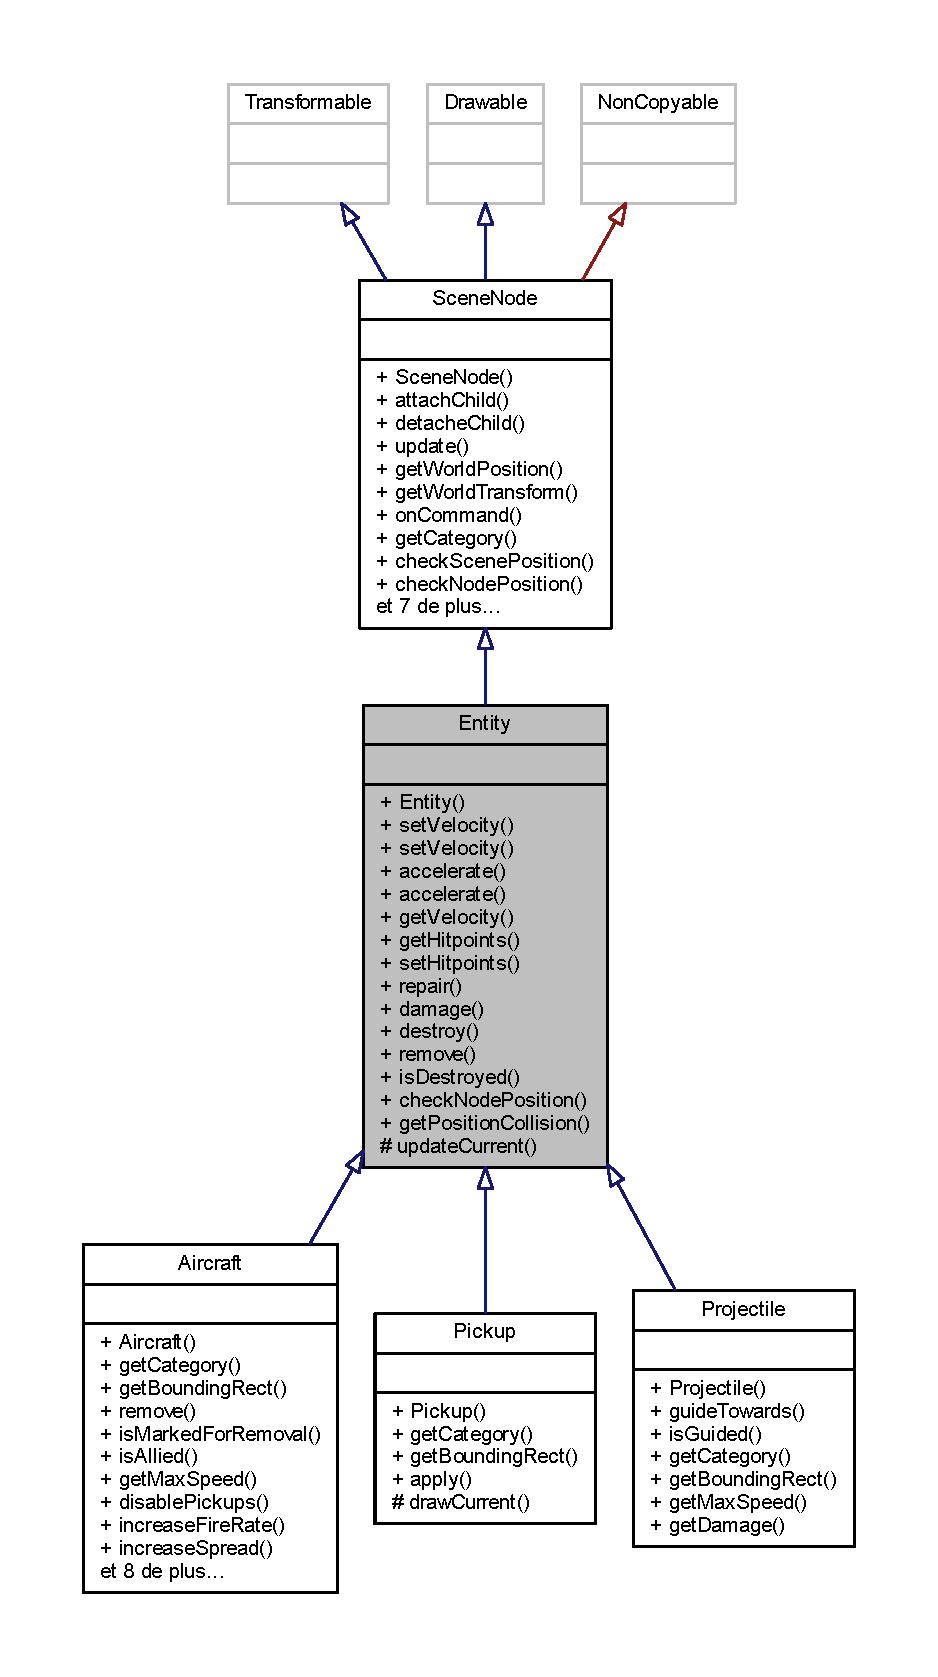
\includegraphics[height=550pt]{class_entity__inherit__graph}
\end{center}
\end{figure}


Graphe de collaboration de Entity\+:\nopagebreak
\begin{figure}[H]
\begin{center}
\leavevmode
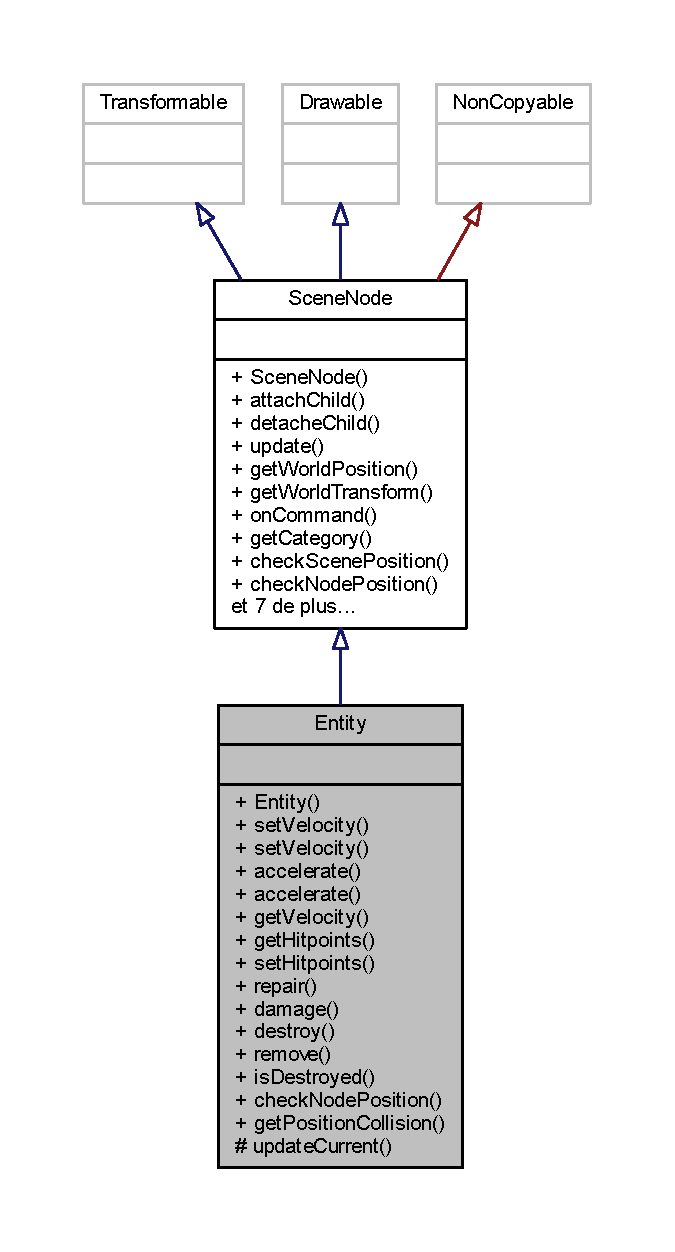
\includegraphics[height=550pt]{class_entity__coll__graph}
\end{center}
\end{figure}
\subsection*{Fonctions membres publiques}
\begin{DoxyCompactItemize}
\item 
\hyperlink{class_entity_a305ac3dd729c288ab23db531fa3fb7e6}{Entity} (int hitpoints)
\begin{DoxyCompactList}\small\item\em Constructeur. \end{DoxyCompactList}\item 
\hypertarget{class_entity_a5bf79843c973eac1fdbebfd1fc83a1e8}{}\label{class_entity_a5bf79843c973eac1fdbebfd1fc83a1e8} 
void {\bfseries set\+Velocity} (sf\+::\+Vector2f velocity)
\item 
\hypertarget{class_entity_a7873fbd61cf1a742d4492ec438a9ac9f}{}\label{class_entity_a7873fbd61cf1a742d4492ec438a9ac9f} 
void {\bfseries set\+Velocity} (float vx, float vy)
\item 
\hypertarget{class_entity_a80cdb89f11d47716781bc567efd2bcda}{}\label{class_entity_a80cdb89f11d47716781bc567efd2bcda} 
void {\bfseries accelerate} (sf\+::\+Vector2f velocity)
\item 
\hypertarget{class_entity_a2ff2403c455f15b3fe5d04e922b3943d}{}\label{class_entity_a2ff2403c455f15b3fe5d04e922b3943d} 
void {\bfseries accelerate} (float vx, float vy)
\item 
\hypertarget{class_entity_ae7518a0181de088e0de2eacd1a13d656}{}\label{class_entity_ae7518a0181de088e0de2eacd1a13d656} 
sf\+::\+Vector2f {\bfseries get\+Velocity} () const
\item 
\hypertarget{class_entity_ade4af3619c02f07429981259bacc881b}{}\label{class_entity_ade4af3619c02f07429981259bacc881b} 
int {\bfseries get\+Hitpoints} () const
\item 
\hypertarget{class_entity_a8791dc8f8c8b944555d67c1aa5dc245d}{}\label{class_entity_a8791dc8f8c8b944555d67c1aa5dc245d} 
void {\bfseries set\+Hitpoints} (int points)
\item 
\hypertarget{class_entity_a354ea9f771b0758f8e70bdfac9a740b4}{}\label{class_entity_a354ea9f771b0758f8e70bdfac9a740b4} 
void {\bfseries repair} (int points)
\item 
\hypertarget{class_entity_a15660fa13012dbca80c8047e2cc6f1f5}{}\label{class_entity_a15660fa13012dbca80c8047e2cc6f1f5} 
void {\bfseries damage} (int points)
\item 
\hypertarget{class_entity_a691dbe5f9ec930c27af2af0b97907a9e}{}\label{class_entity_a691dbe5f9ec930c27af2af0b97907a9e} 
void {\bfseries destroy} ()
\item 
\hypertarget{class_entity_aa84c32a5d1baceccefec62568edc0a4f}{}\label{class_entity_aa84c32a5d1baceccefec62568edc0a4f} 
virtual void {\bfseries remove} ()
\item 
\hypertarget{class_entity_a938cddf03ff5239be09195452142c5e6}{}\label{class_entity_a938cddf03ff5239be09195452142c5e6} 
virtual bool {\bfseries is\+Destroyed} () const
\item 
\hypertarget{class_entity_a4ffae7e910fc9deaabfed51d014ff1db}{}\label{class_entity_a4ffae7e910fc9deaabfed51d014ff1db} 
virtual void {\bfseries check\+Node\+Position} (\hyperlink{class_scene_node}{Scene\+Node} \&node, const std\+::vector$<$ sf\+::\+Float\+Rect $>$ \&virtual\+Rect\+Collision, std\+::multimap$<$ int, \hyperlink{class_scene_node}{Scene\+Node} $\ast$$>$ \&collision\+Liste\+To\+Test, sf\+::\+Int32 nb\+CutX, sf\+::\+Int32 nb\+CutY)
\item 
\hypertarget{class_entity_abb13dc0928903ef41dab61858b7220d4}{}\label{class_entity_abb13dc0928903ef41dab61858b7220d4} 
virtual int {\bfseries get\+Position\+Collision} () const
\end{DoxyCompactItemize}
\subsection*{Fonctions membres protégées}
\begin{DoxyCompactItemize}
\item 
\hypertarget{class_entity_a3d9ad14643b61864cf60ea7f0738146b}{}\label{class_entity_a3d9ad14643b61864cf60ea7f0738146b} 
virtual void {\bfseries update\+Current} (sf\+::\+Time dt, \hyperlink{class_command_queue}{Command\+Queue} \&commands)
\end{DoxyCompactItemize}
\subsection*{Membres hérités additionnels}


\subsection{Description détaillée}
Classe representant l\textquotesingle{}entit�e 

La classe g�re les entit�es 

Définition à la ligne 21 du fichier Entity.\+h.



\subsection{Documentation des constructeurs et destructeur}
\hypertarget{class_entity_a305ac3dd729c288ab23db531fa3fb7e6}{}\label{class_entity_a305ac3dd729c288ab23db531fa3fb7e6} 
\index{Entity@{Entity}!Entity@{Entity}}
\index{Entity@{Entity}!Entity@{Entity}}
\subsubsection{\texorpdfstring{Entity()}{Entity()}}
{\footnotesize\ttfamily Entity\+::\+Entity (\begin{DoxyParamCaption}\item[{int}]{hitpoints }\end{DoxyParamCaption})\hspace{0.3cm}{\ttfamily [explicit]}}



Constructeur. 


\begin{DoxyParams}{Paramètres}
{\em hitpoints} & \+: Nombre de point de vie de l\textquotesingle{}entit�e \\
\hline
\end{DoxyParams}


Définition à la ligne 6 du fichier Entity.\+cpp.



La documentation de cette classe a été générée à partir des fichiers suivants \+:\begin{DoxyCompactItemize}
\item 
\hyperlink{_entity_8h}{Entity.\+h}\item 
Entity.\+cpp\end{DoxyCompactItemize}

\hypertarget{class_game_over_state}{}\section{Référence de la classe Game\+Over\+State}
\label{class_game_over_state}\index{Game\+Over\+State@{Game\+Over\+State}}


Graphe d\textquotesingle{}héritage de Game\+Over\+State\+:\nopagebreak
\begin{figure}[H]
\begin{center}
\leavevmode
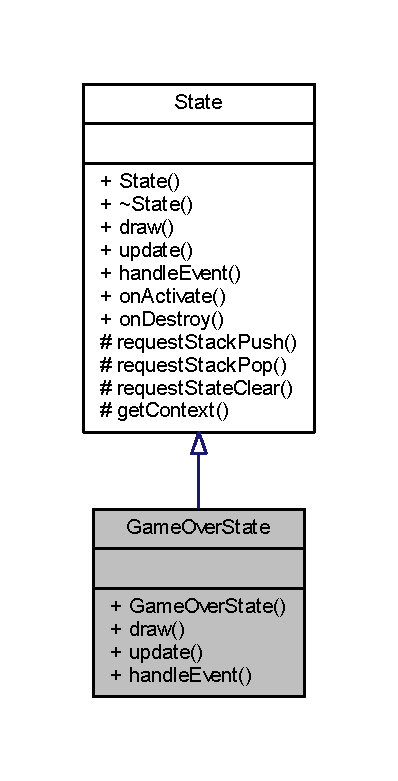
\includegraphics[width=191pt]{class_game_over_state__inherit__graph}
\end{center}
\end{figure}


Graphe de collaboration de Game\+Over\+State\+:\nopagebreak
\begin{figure}[H]
\begin{center}
\leavevmode
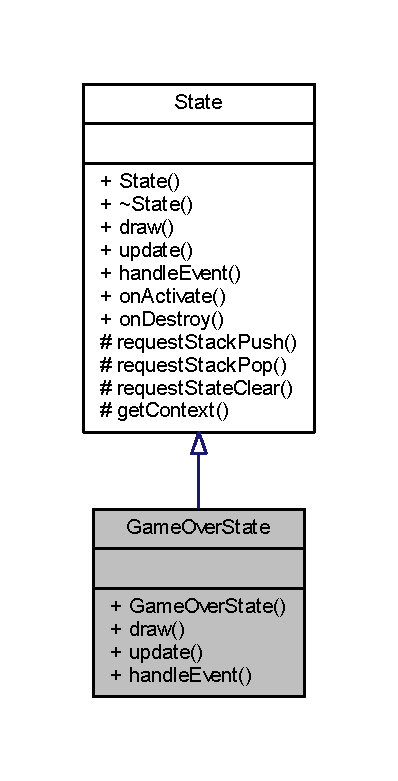
\includegraphics[width=191pt]{class_game_over_state__coll__graph}
\end{center}
\end{figure}
\subsection*{Fonctions membres publiques}
\begin{DoxyCompactItemize}
\item 
\hypertarget{class_game_over_state_a025337813b515023e9bbce92af1c08eb}{}\label{class_game_over_state_a025337813b515023e9bbce92af1c08eb} 
{\bfseries Game\+Over\+State} (\hyperlink{class_state_stack}{State\+Stack} \&stack, \hyperlink{struct_state_1_1_context}{Context} context, const std\+::string \&text)
\item 
\hypertarget{class_game_over_state_a9decc1411647e390bfed0bdc009cd691}{}\label{class_game_over_state_a9decc1411647e390bfed0bdc009cd691} 
virtual void {\bfseries draw} ()
\item 
\hypertarget{class_game_over_state_a8a2047b5c684965f33574b8aee7b7c8f}{}\label{class_game_over_state_a8a2047b5c684965f33574b8aee7b7c8f} 
virtual bool {\bfseries update} (sf\+::\+Time dt)
\item 
\hypertarget{class_game_over_state_acf1dc2c7f58fe21b7cfababaf87ff20b}{}\label{class_game_over_state_acf1dc2c7f58fe21b7cfababaf87ff20b} 
virtual bool {\bfseries handle\+Event} (const sf\+::\+Event \&event)
\end{DoxyCompactItemize}
\subsection*{Membres hérités additionnels}


\subsection{Description détaillée}


Définition à la ligne 11 du fichier Game\+Over\+State.\+h.



La documentation de cette classe a été générée à partir des fichiers suivants \+:\begin{DoxyCompactItemize}
\item 
Game\+Over\+State.\+h\item 
Game\+Over\+State.\+cpp\end{DoxyCompactItemize}

\hypertarget{class_game_server}{}\section{Référence de la classe Game\+Server}
\label{class_game_server}\index{Game\+Server@{Game\+Server}}


Graphe de collaboration de Game\+Server\+:\nopagebreak
\begin{figure}[H]
\begin{center}
\leavevmode
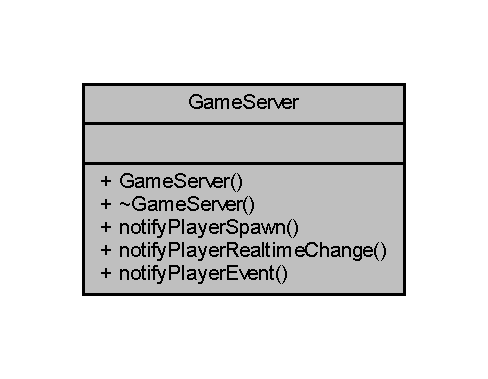
\includegraphics[width=234pt]{class_game_server__coll__graph}
\end{center}
\end{figure}
\subsection*{Fonctions membres publiques}
\begin{DoxyCompactItemize}
\item 
\hypertarget{class_game_server_a61393ed81464c44e95784b4c3f49f19c}{}\label{class_game_server_a61393ed81464c44e95784b4c3f49f19c} 
{\bfseries Game\+Server} (sf\+::\+Vector2f battlefield\+Size)
\item 
\hypertarget{class_game_server_a3a0a351ef8758c358f7e9cbdee82889c}{}\label{class_game_server_a3a0a351ef8758c358f7e9cbdee82889c} 
void {\bfseries notify\+Player\+Spawn} (sf\+::\+Int32 aircraft\+Identifier)
\item 
\hypertarget{class_game_server_ab785edd984324549e033677f35dd025e}{}\label{class_game_server_ab785edd984324549e033677f35dd025e} 
void {\bfseries notify\+Player\+Realtime\+Change} (sf\+::\+Int32 aircraft\+Identifier, sf\+::\+Int32 action, bool action\+Enable)
\item 
\hypertarget{class_game_server_add73992b0e7cb29ebbfc745a4f79155e}{}\label{class_game_server_add73992b0e7cb29ebbfc745a4f79155e} 
void {\bfseries notify\+Player\+Event} (sf\+::\+Int32 aircraft\+Identifier, sf\+::\+Int32 action)
\end{DoxyCompactItemize}


\subsection{Description détaillée}


Définition à la ligne 17 du fichier Game\+Server.\+h.



La documentation de cette classe a été générée à partir des fichiers suivants \+:\begin{DoxyCompactItemize}
\item 
Game\+Server.\+h\item 
Game\+Server.\+cpp\end{DoxyCompactItemize}

\hypertarget{class_game_state}{}\section{Référence de la classe Game\+State}
\label{class_game_state}\index{Game\+State@{Game\+State}}


Graphe d\textquotesingle{}héritage de Game\+State\+:\nopagebreak
\begin{figure}[H]
\begin{center}
\leavevmode
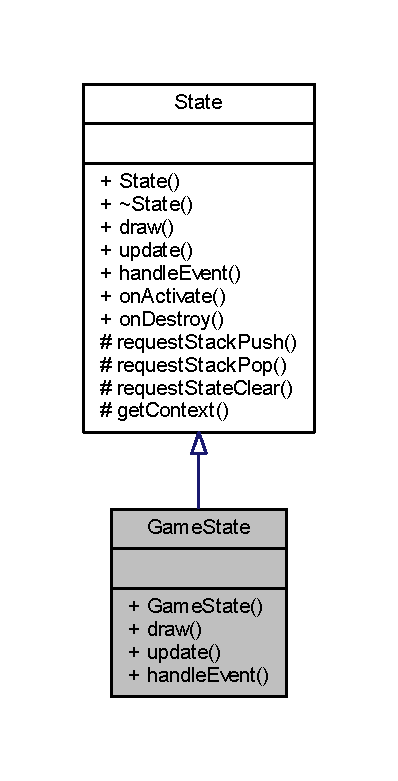
\includegraphics[width=191pt]{class_game_state__inherit__graph}
\end{center}
\end{figure}


Graphe de collaboration de Game\+State\+:\nopagebreak
\begin{figure}[H]
\begin{center}
\leavevmode
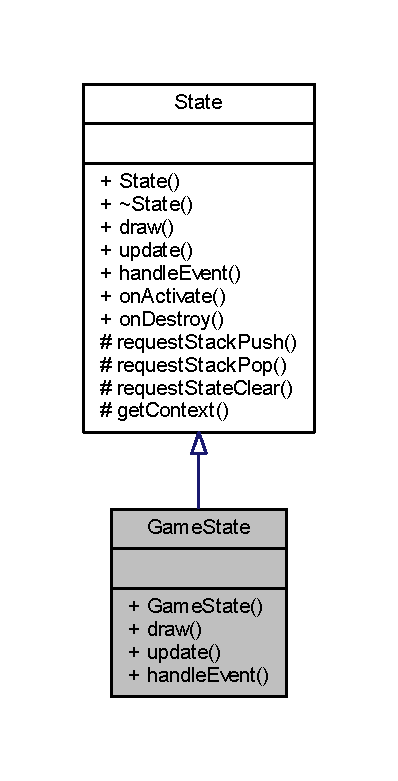
\includegraphics[width=191pt]{class_game_state__coll__graph}
\end{center}
\end{figure}
\subsection*{Fonctions membres publiques}
\begin{DoxyCompactItemize}
\item 
{\bfseries Game\+State} (\hyperlink{class_state_stack}{State\+Stack} \&stack, \hyperlink{struct_state_1_1_context}{Context} context)\hypertarget{class_game_state_aeb2e2598754640c694b989311b1aebfe}{}\label{class_game_state_aeb2e2598754640c694b989311b1aebfe}

\item 
virtual void {\bfseries draw} ()\hypertarget{class_game_state_a3c511417d8934943ae65c04681f321a3}{}\label{class_game_state_a3c511417d8934943ae65c04681f321a3}

\item 
virtual bool {\bfseries update} (sf\+::\+Time dt)\hypertarget{class_game_state_a4ac988f0da5c33b43ff356890fcf9c1c}{}\label{class_game_state_a4ac988f0da5c33b43ff356890fcf9c1c}

\item 
virtual bool {\bfseries handle\+Event} (const sf\+::\+Event \&event)\hypertarget{class_game_state_a000dd3306b1cb9faab5a86774a22aa6d}{}\label{class_game_state_a000dd3306b1cb9faab5a86774a22aa6d}

\end{DoxyCompactItemize}
\subsection*{Membres hérités additionnels}


La documentation de cette classe a été générée à partir des fichiers suivants \+:\begin{DoxyCompactItemize}
\item 
C\+:/\+Users/\+F\+R\+E\+D/\+Documents/\+F\+R\+E\+D/\+Programmation\+\_\+jeux/\+Projet\+\_\+\+S\+F\+M\+L/\+Projet2/include/Game\+State.\+h\item 
C\+:/\+Users/\+F\+R\+E\+D/\+Documents/\+F\+R\+E\+D/\+Programmation\+\_\+jeux/\+Projet\+\_\+\+S\+F\+M\+L/\+Projet2/src/Game\+State.\+cpp\end{DoxyCompactItemize}

\hypertarget{class_key_binding}{}\section{Référence de la classe Key\+Binding}
\label{class_key_binding}\index{Key\+Binding@{Key\+Binding}}


Graphe de collaboration de Key\+Binding\+:\nopagebreak
\begin{figure}[H]
\begin{center}
\leavevmode
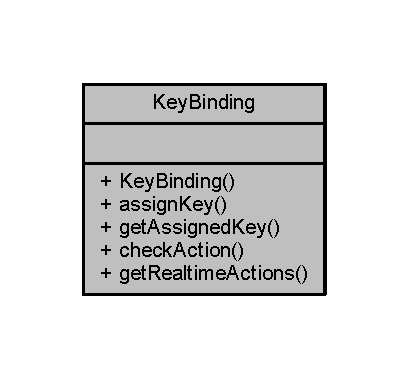
\includegraphics[width=196pt]{class_key_binding__coll__graph}
\end{center}
\end{figure}
\subsection*{Types publics}
\begin{DoxyCompactItemize}
\item 
\hypertarget{class_key_binding_aa7d3e2787c3e4d64d2cc6c9403681db0}{}\label{class_key_binding_aa7d3e2787c3e4d64d2cc6c9403681db0} 
typedef Player\+Action\+::\+Type {\bfseries Action}
\end{DoxyCompactItemize}
\subsection*{Fonctions membres publiques}
\begin{DoxyCompactItemize}
\item 
\hypertarget{class_key_binding_aa343e67d4fc402a18994359a8d064df3}{}\label{class_key_binding_aa343e67d4fc402a18994359a8d064df3} 
{\bfseries Key\+Binding} (int control\+Preconfiguration)
\item 
\hypertarget{class_key_binding_a88b4df445ff9d050723710cd75a8cd3f}{}\label{class_key_binding_a88b4df445ff9d050723710cd75a8cd3f} 
void {\bfseries assign\+Key} (Action action, sf\+::\+Keyboard\+::\+Key key)
\item 
\hypertarget{class_key_binding_af55da9ca1a666a2617b7f32a51e1b466}{}\label{class_key_binding_af55da9ca1a666a2617b7f32a51e1b466} 
sf\+::\+Keyboard\+::\+Key {\bfseries get\+Assigned\+Key} (Action action) const
\item 
\hypertarget{class_key_binding_aa11ef504d52c2a05e2a43bc833f28408}{}\label{class_key_binding_aa11ef504d52c2a05e2a43bc833f28408} 
bool {\bfseries check\+Action} (sf\+::\+Keyboard\+::\+Key key, Action \&out) const
\item 
\hypertarget{class_key_binding_a990f9e66f5bc5f07fbd7ef38c1fba64b}{}\label{class_key_binding_a990f9e66f5bc5f07fbd7ef38c1fba64b} 
std\+::vector$<$ Action $>$ {\bfseries get\+Realtime\+Actions} () const
\end{DoxyCompactItemize}


\subsection{Description détaillée}


Définition à la ligne 23 du fichier Key\+Binding.\+h.



La documentation de cette classe a été générée à partir des fichiers suivants \+:\begin{DoxyCompactItemize}
\item 
Key\+Binding.\+h\item 
Key\+Binding.\+cpp\end{DoxyCompactItemize}

\hypertarget{class_g_u_i_1_1_label}{}\section{Référence de la classe G\+UI\+:\+:Label}
\label{class_g_u_i_1_1_label}\index{G\+U\+I\+::\+Label@{G\+U\+I\+::\+Label}}


Graphe d\textquotesingle{}héritage de G\+UI\+:\+:Label\+:\nopagebreak
\begin{figure}[H]
\begin{center}
\leavevmode
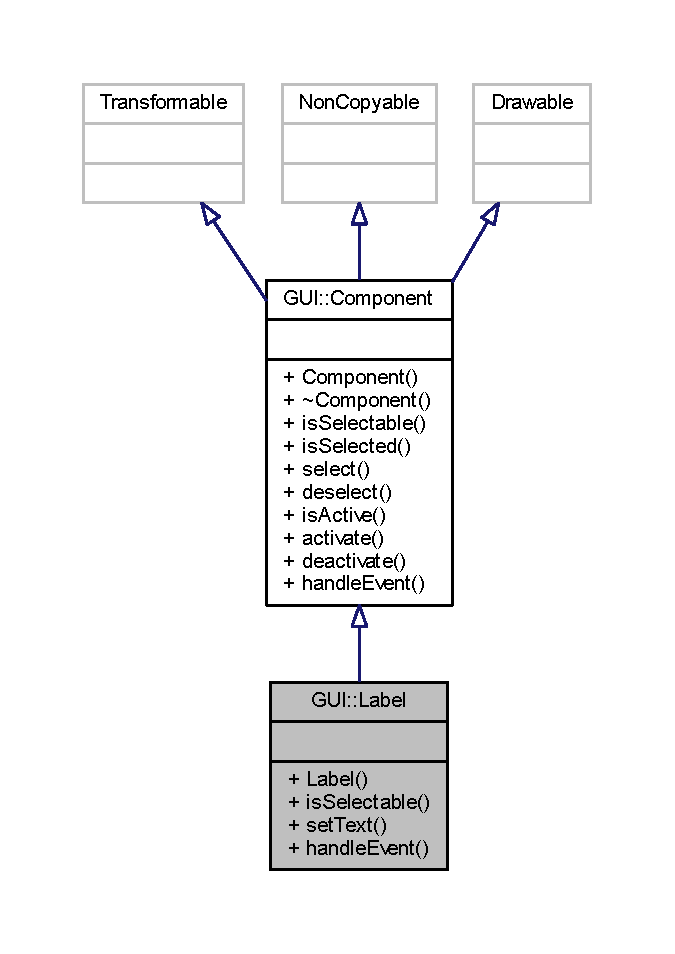
\includegraphics[width=324pt]{class_g_u_i_1_1_label__inherit__graph}
\end{center}
\end{figure}


Graphe de collaboration de G\+UI\+:\+:Label\+:\nopagebreak
\begin{figure}[H]
\begin{center}
\leavevmode
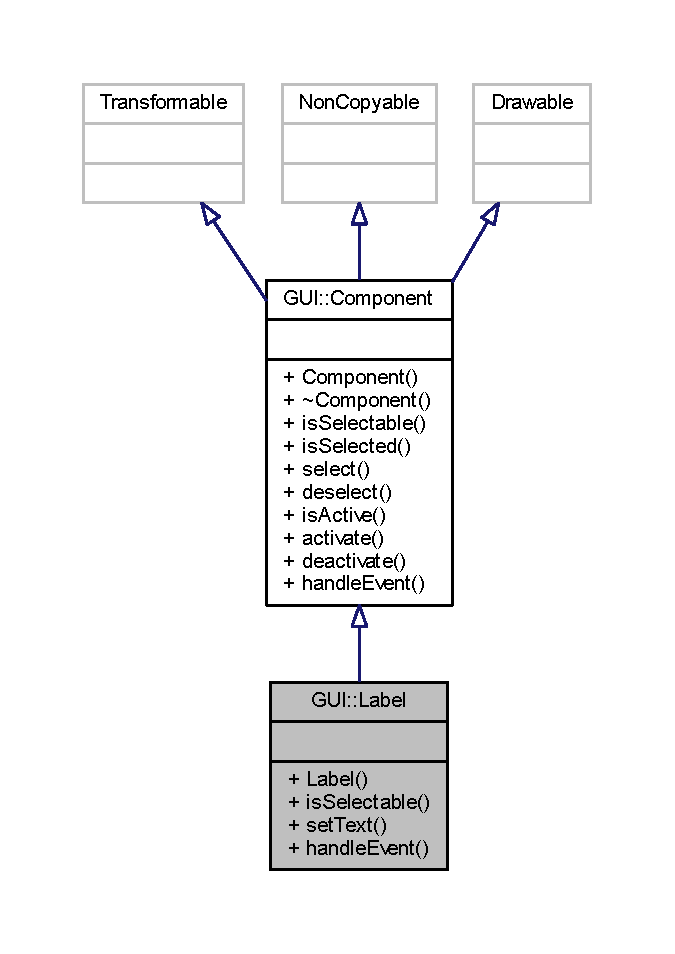
\includegraphics[width=324pt]{class_g_u_i_1_1_label__coll__graph}
\end{center}
\end{figure}
\subsection*{Types publics}
\begin{DoxyCompactItemize}
\item 
\hypertarget{class_g_u_i_1_1_label_aa00f786f8578a677ef7b979aa28c2546}{}\label{class_g_u_i_1_1_label_aa00f786f8578a677ef7b979aa28c2546} 
typedef std\+::shared\+\_\+ptr$<$ \hyperlink{class_g_u_i_1_1_label}{Label} $>$ {\bfseries Ptr}
\end{DoxyCompactItemize}
\subsection*{Fonctions membres publiques}
\begin{DoxyCompactItemize}
\item 
\hypertarget{class_g_u_i_1_1_label_af7776f7b27736bf53a41b8aec79a60c5}{}\label{class_g_u_i_1_1_label_af7776f7b27736bf53a41b8aec79a60c5} 
{\bfseries Label} (const std\+::string \&text, const \hyperlink{class_resource_holder}{Font\+Holder} \&fonts)
\item 
\hypertarget{class_g_u_i_1_1_label_a93581f2d9ba05972df01788f8c9ad4ac}{}\label{class_g_u_i_1_1_label_a93581f2d9ba05972df01788f8c9ad4ac} 
virtual bool {\bfseries is\+Selectable} () const
\item 
\hypertarget{class_g_u_i_1_1_label_ab86467acdbe18a9fda4712a177e16dae}{}\label{class_g_u_i_1_1_label_ab86467acdbe18a9fda4712a177e16dae} 
void {\bfseries set\+Text} (const std\+::string \&text)
\item 
\hypertarget{class_g_u_i_1_1_label_ade8d6fc5a2f56198764ee0ee0f216068}{}\label{class_g_u_i_1_1_label_ade8d6fc5a2f56198764ee0ee0f216068} 
virtual void {\bfseries handle\+Event} (const sf\+::\+Event \&event)
\end{DoxyCompactItemize}


\subsection{Description détaillée}


Définition à la ligne 13 du fichier Label.\+h.



La documentation de cette classe a été générée à partir des fichiers suivants \+:\begin{DoxyCompactItemize}
\item 
Label.\+h\item 
Label.\+cpp\end{DoxyCompactItemize}

\hypertarget{class_loading_state}{}\section{Référence de la classe Loading\+State}
\label{class_loading_state}\index{Loading\+State@{Loading\+State}}


Graphe d\textquotesingle{}héritage de Loading\+State\+:\nopagebreak
\begin{figure}[H]
\begin{center}
\leavevmode
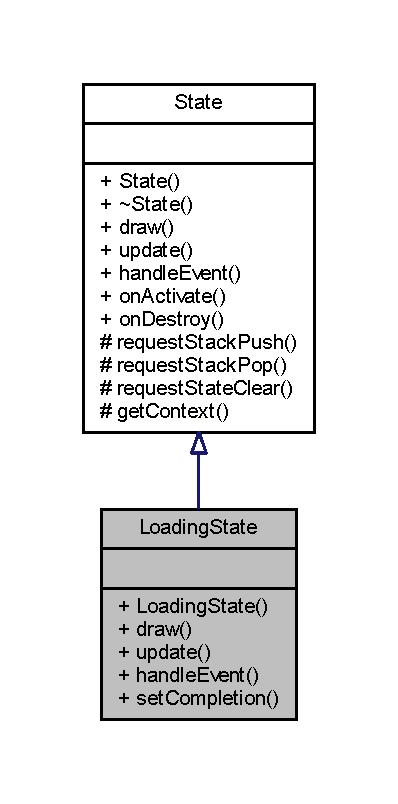
\includegraphics[width=191pt]{class_loading_state__inherit__graph}
\end{center}
\end{figure}


Graphe de collaboration de Loading\+State\+:\nopagebreak
\begin{figure}[H]
\begin{center}
\leavevmode
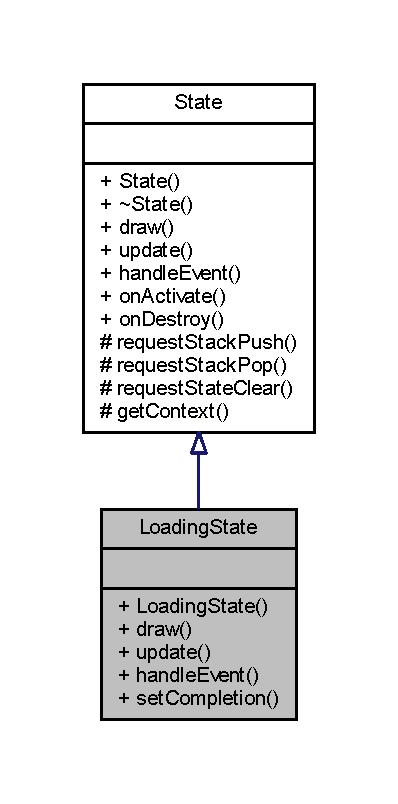
\includegraphics[width=191pt]{class_loading_state__coll__graph}
\end{center}
\end{figure}
\subsection*{Fonctions membres publiques}
\begin{DoxyCompactItemize}
\item 
\hypertarget{class_loading_state_a6830cacada1f9c215f913d31aa1805cf}{}\label{class_loading_state_a6830cacada1f9c215f913d31aa1805cf} 
{\bfseries Loading\+State} (\hyperlink{class_state_stack}{State\+Stack} \&stack, \hyperlink{struct_state_1_1_context}{Context} context)
\item 
\hypertarget{class_loading_state_adfe2c002c52cc2c49967ba3ace4aa73b}{}\label{class_loading_state_adfe2c002c52cc2c49967ba3ace4aa73b} 
virtual void {\bfseries draw} ()
\item 
\hypertarget{class_loading_state_a8f2f50523c1f35e011ddd0839aa66ee4}{}\label{class_loading_state_a8f2f50523c1f35e011ddd0839aa66ee4} 
virtual bool {\bfseries update} (sf\+::\+Time dt)
\item 
\hypertarget{class_loading_state_a37da243eeeca36460bac2f32cef3e368}{}\label{class_loading_state_a37da243eeeca36460bac2f32cef3e368} 
virtual bool {\bfseries handle\+Event} (const sf\+::\+Event \&event)
\item 
\hypertarget{class_loading_state_a28bee93e7f9818084af8be6b31ee0ba4}{}\label{class_loading_state_a28bee93e7f9818084af8be6b31ee0ba4} 
void {\bfseries set\+Completion} (float percent)
\end{DoxyCompactItemize}
\subsection*{Membres hérités additionnels}


\subsection{Description détaillée}


Définition à la ligne 13 du fichier Loading\+State.\+h.



La documentation de cette classe a été générée à partir des fichiers suivants \+:\begin{DoxyCompactItemize}
\item 
Loading\+State.\+h\item 
Loading\+State.\+cpp\end{DoxyCompactItemize}

\hypertarget{class_menu_state}{}\section{Référence de la classe Menu\+State}
\label{class_menu_state}\index{Menu\+State@{Menu\+State}}


Graphe d\textquotesingle{}héritage de Menu\+State\+:\nopagebreak
\begin{figure}[H]
\begin{center}
\leavevmode
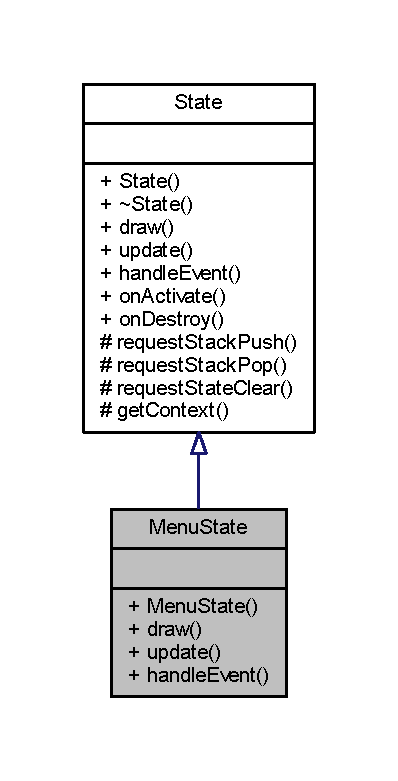
\includegraphics[width=191pt]{class_menu_state__inherit__graph}
\end{center}
\end{figure}


Graphe de collaboration de Menu\+State\+:\nopagebreak
\begin{figure}[H]
\begin{center}
\leavevmode
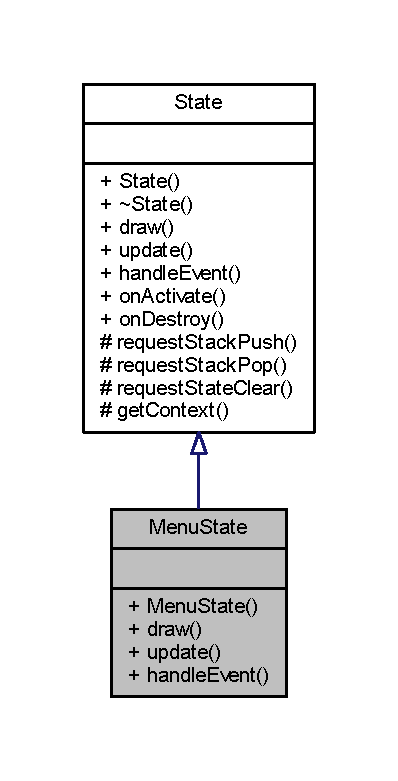
\includegraphics[width=191pt]{class_menu_state__coll__graph}
\end{center}
\end{figure}
\subsection*{Fonctions membres publiques}
\begin{DoxyCompactItemize}
\item 
\hypertarget{class_menu_state_a6e7034c57bf83f24aa8f4321d3d210a5}{}\label{class_menu_state_a6e7034c57bf83f24aa8f4321d3d210a5} 
{\bfseries Menu\+State} (\hyperlink{class_state_stack}{State\+Stack} \&stack, \hyperlink{struct_state_1_1_context}{Context} context)
\item 
\hypertarget{class_menu_state_aa557d6c3bf06bb3107ed780913a6b47f}{}\label{class_menu_state_aa557d6c3bf06bb3107ed780913a6b47f} 
virtual void {\bfseries draw} ()
\item 
\hypertarget{class_menu_state_adac67748651bd33ddadb36a4f8a246da}{}\label{class_menu_state_adac67748651bd33ddadb36a4f8a246da} 
virtual bool {\bfseries update} (sf\+::\+Time dt)
\item 
\hypertarget{class_menu_state_a04a21241cebf6a8f0fe8ee9ce895ef18}{}\label{class_menu_state_a04a21241cebf6a8f0fe8ee9ce895ef18} 
virtual bool {\bfseries handle\+Event} (const sf\+::\+Event \&event)
\end{DoxyCompactItemize}
\subsection*{Membres hérités additionnels}


\subsection{Description détaillée}


Définition à la ligne 10 du fichier Menu\+State.\+h.



La documentation de cette classe a été générée à partir des fichiers suivants \+:\begin{DoxyCompactItemize}
\item 
Menu\+State.\+h\item 
Menu\+State.\+cpp\end{DoxyCompactItemize}

\hypertarget{class_multiplayer_game_state}{}\section{Référence de la classe Multiplayer\+Game\+State}
\label{class_multiplayer_game_state}\index{Multiplayer\+Game\+State@{Multiplayer\+Game\+State}}


Graphe d\textquotesingle{}héritage de Multiplayer\+Game\+State\+:\nopagebreak
\begin{figure}[H]
\begin{center}
\leavevmode
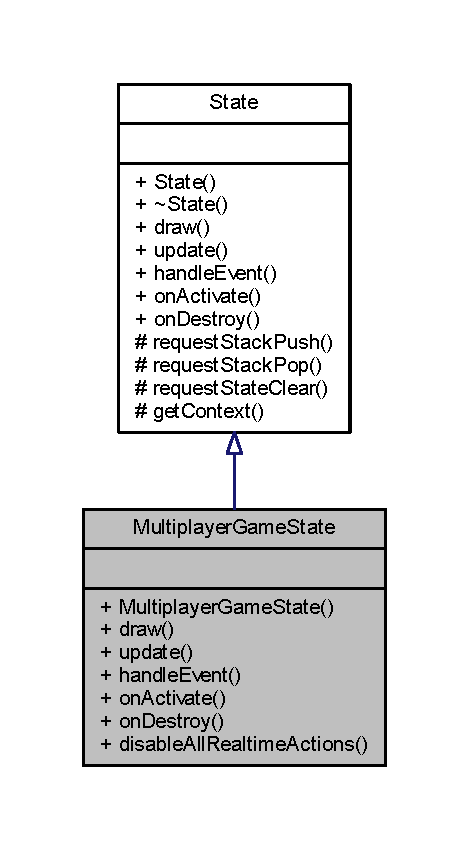
\includegraphics[width=225pt]{class_multiplayer_game_state__inherit__graph}
\end{center}
\end{figure}


Graphe de collaboration de Multiplayer\+Game\+State\+:\nopagebreak
\begin{figure}[H]
\begin{center}
\leavevmode
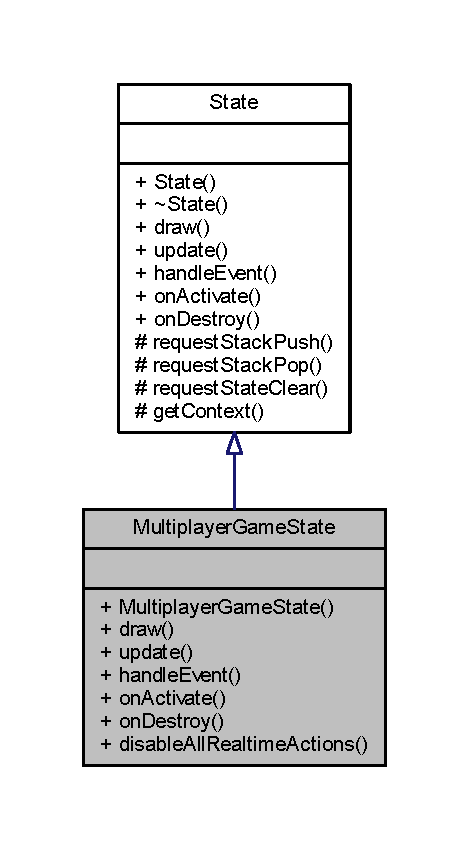
\includegraphics[width=225pt]{class_multiplayer_game_state__coll__graph}
\end{center}
\end{figure}
\subsection*{Fonctions membres publiques}
\begin{DoxyCompactItemize}
\item 
\hypertarget{class_multiplayer_game_state_abdff9f279bb851861d1dbba9cf33d90b}{}\label{class_multiplayer_game_state_abdff9f279bb851861d1dbba9cf33d90b} 
{\bfseries Multiplayer\+Game\+State} (\hyperlink{class_state_stack}{State\+Stack} \&stack, \hyperlink{struct_state_1_1_context}{Context} context, bool is\+Host)
\item 
\hypertarget{class_multiplayer_game_state_a629171643cccd9c8914b50971a9dc940}{}\label{class_multiplayer_game_state_a629171643cccd9c8914b50971a9dc940} 
virtual void {\bfseries draw} ()
\item 
\hypertarget{class_multiplayer_game_state_a5affe4cb62f5acadcdb9b81d1766ad6a}{}\label{class_multiplayer_game_state_a5affe4cb62f5acadcdb9b81d1766ad6a} 
virtual bool {\bfseries update} (sf\+::\+Time dt)
\item 
\hypertarget{class_multiplayer_game_state_a27489fecf201c5dfd5f046f0e4f813b5}{}\label{class_multiplayer_game_state_a27489fecf201c5dfd5f046f0e4f813b5} 
virtual bool {\bfseries handle\+Event} (const sf\+::\+Event \&event)
\item 
\hypertarget{class_multiplayer_game_state_ae4f04690436f735755228e98c99f4b4f}{}\label{class_multiplayer_game_state_ae4f04690436f735755228e98c99f4b4f} 
virtual void {\bfseries on\+Activate} ()
\item 
\hypertarget{class_multiplayer_game_state_afb40e8a952b1f6264e688b80fc894bde}{}\label{class_multiplayer_game_state_afb40e8a952b1f6264e688b80fc894bde} 
void {\bfseries on\+Destroy} ()
\item 
\hypertarget{class_multiplayer_game_state_aae8391f9b734eb396bc5340d131f4441}{}\label{class_multiplayer_game_state_aae8391f9b734eb396bc5340d131f4441} 
void {\bfseries disable\+All\+Realtime\+Actions} ()
\end{DoxyCompactItemize}
\subsection*{Membres hérités additionnels}


\subsection{Description détaillée}


Définition à la ligne 16 du fichier Multiplayer\+Game\+State.\+h.



La documentation de cette classe a été générée à partir des fichiers suivants \+:\begin{DoxyCompactItemize}
\item 
Multiplayer\+Game\+State.\+h\item 
Multiplayer\+Game\+State.\+cpp\end{DoxyCompactItemize}

\hypertarget{class_music_player}{}\section{Référence de la classe Music\+Player}
\label{class_music_player}\index{Music\+Player@{Music\+Player}}


Graphe d\textquotesingle{}héritage de Music\+Player\+:\nopagebreak
\begin{figure}[H]
\begin{center}
\leavevmode
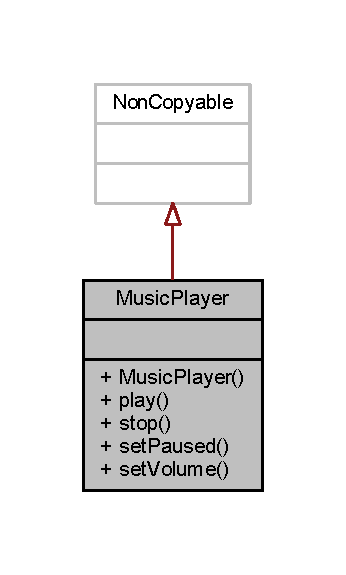
\includegraphics[width=166pt]{class_music_player__inherit__graph}
\end{center}
\end{figure}


Graphe de collaboration de Music\+Player\+:\nopagebreak
\begin{figure}[H]
\begin{center}
\leavevmode
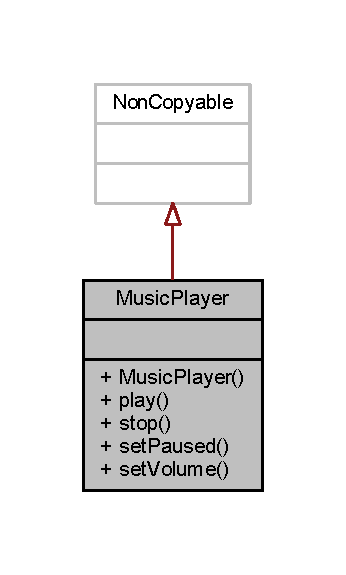
\includegraphics[width=166pt]{class_music_player__coll__graph}
\end{center}
\end{figure}
\subsection*{Fonctions membres publiques}
\begin{DoxyCompactItemize}
\item 
\hypertarget{class_music_player_a8a10a649154c8b7af3031c5f36cb53ca}{}\label{class_music_player_a8a10a649154c8b7af3031c5f36cb53ca} 
void {\bfseries play} (Music\+::\+ID theme)
\item 
\hypertarget{class_music_player_a54e47a9e937730493d886aa5624c44d1}{}\label{class_music_player_a54e47a9e937730493d886aa5624c44d1} 
void {\bfseries stop} ()
\item 
\hypertarget{class_music_player_a59b313a9a9eb850e590f9c6555ad80cf}{}\label{class_music_player_a59b313a9a9eb850e590f9c6555ad80cf} 
void {\bfseries set\+Paused} (bool paused)
\item 
\hypertarget{class_music_player_a361cbcbfb31d3c0c841d0b67a79c5cdd}{}\label{class_music_player_a361cbcbfb31d3c0c841d0b67a79c5cdd} 
void {\bfseries set\+Volume} (float volume)
\end{DoxyCompactItemize}


\subsection{Description détaillée}


Définition à la ligne 13 du fichier Music\+Player.\+h.



La documentation de cette classe a été générée à partir des fichiers suivants \+:\begin{DoxyCompactItemize}
\item 
Music\+Player.\+h\item 
Music\+Player.\+cpp\end{DoxyCompactItemize}

\hypertarget{class_network_node}{}\section{Référence de la classe Network\+Node}
\label{class_network_node}\index{Network\+Node@{Network\+Node}}


Graphe d\textquotesingle{}héritage de Network\+Node\+:\nopagebreak
\begin{figure}[H]
\begin{center}
\leavevmode
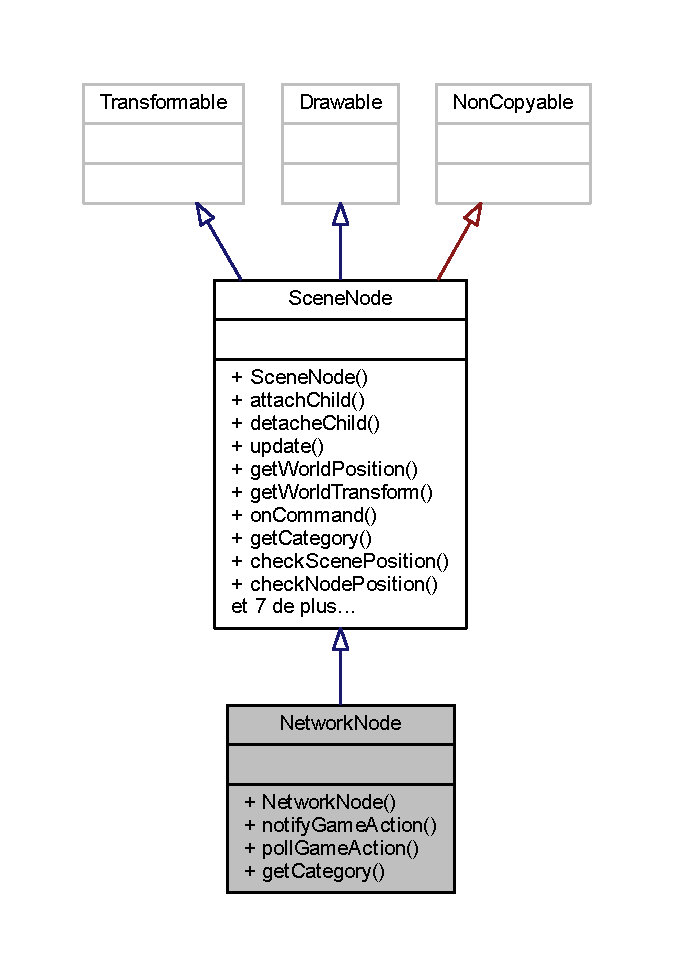
\includegraphics[width=324pt]{class_network_node__inherit__graph}
\end{center}
\end{figure}


Graphe de collaboration de Network\+Node\+:\nopagebreak
\begin{figure}[H]
\begin{center}
\leavevmode
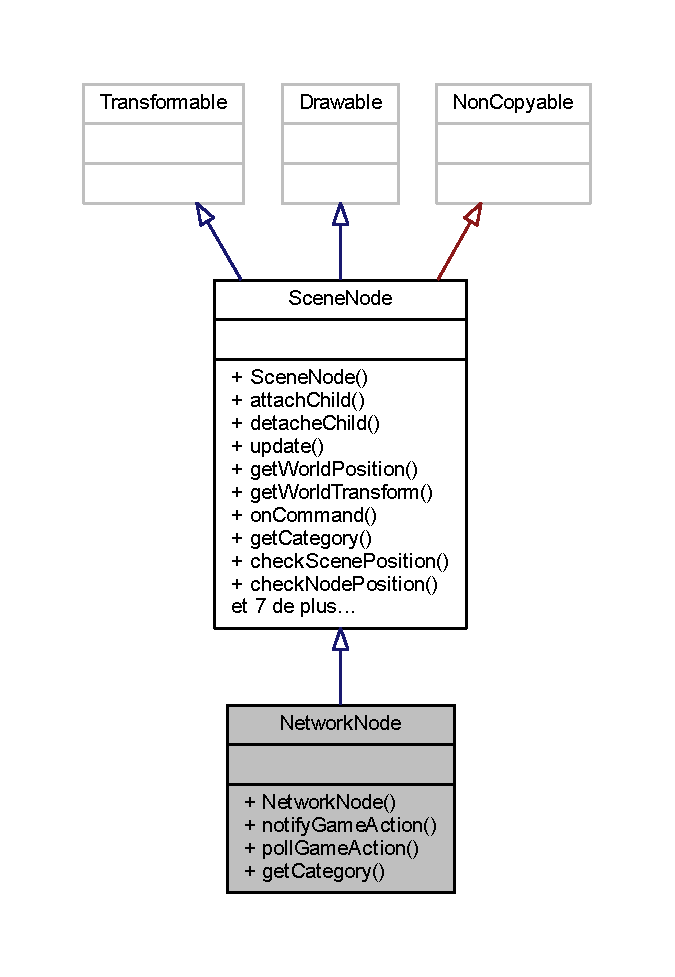
\includegraphics[width=324pt]{class_network_node__coll__graph}
\end{center}
\end{figure}
\subsection*{Fonctions membres publiques}
\begin{DoxyCompactItemize}
\item 
\hypertarget{class_network_node_a76c8daddb63d9d2ea57a1e3096b0fcc1}{}\label{class_network_node_a76c8daddb63d9d2ea57a1e3096b0fcc1} 
void {\bfseries notify\+Game\+Action} (Game\+Actions\+::\+Type type, sf\+::\+Vector2f position)
\item 
\hypertarget{class_network_node_a324d5374146ccb8e1a77c932623464c1}{}\label{class_network_node_a324d5374146ccb8e1a77c932623464c1} 
bool {\bfseries poll\+Game\+Action} (\hyperlink{struct_game_actions_1_1_action}{Game\+Actions\+::\+Action} \&out)
\item 
\hypertarget{class_network_node_aae5b3c7b6f20f4a5ba695957b51e52bc}{}\label{class_network_node_aae5b3c7b6f20f4a5ba695957b51e52bc} 
virtual unsigned int {\bfseries get\+Category} () const
\end{DoxyCompactItemize}
\subsection*{Membres hérités additionnels}


\subsection{Description détaillée}


Définition à la ligne 9 du fichier Network\+Node.\+h.



La documentation de cette classe a été générée à partir des fichiers suivants \+:\begin{DoxyCompactItemize}
\item 
Network\+Node.\+h\item 
Network\+Node.\+cpp\end{DoxyCompactItemize}

\hypertarget{class_parallel_task}{}\section{Référence de la classe Parallel\+Task}
\label{class_parallel_task}\index{Parallel\+Task@{Parallel\+Task}}


Graphe de collaboration de Parallel\+Task\+:\nopagebreak
\begin{figure}[H]
\begin{center}
\leavevmode
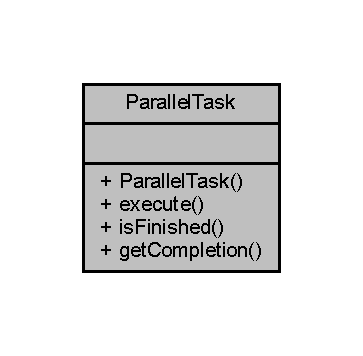
\includegraphics[width=174pt]{class_parallel_task__coll__graph}
\end{center}
\end{figure}
\subsection*{Fonctions membres publiques}
\begin{DoxyCompactItemize}
\item 
void {\bfseries execute} ()\hypertarget{class_parallel_task_ad1e7ba9134cc7961ab178a2f47cf54be}{}\label{class_parallel_task_ad1e7ba9134cc7961ab178a2f47cf54be}

\item 
bool {\bfseries is\+Finished} ()\hypertarget{class_parallel_task_a1a67f547aa382fac2087184b2eb19148}{}\label{class_parallel_task_a1a67f547aa382fac2087184b2eb19148}

\item 
float {\bfseries get\+Completion} ()\hypertarget{class_parallel_task_ada45e4db1aa8a89f20ab0b8662c6dabc}{}\label{class_parallel_task_ada45e4db1aa8a89f20ab0b8662c6dabc}

\end{DoxyCompactItemize}


La documentation de cette classe a été générée à partir des fichiers suivants \+:\begin{DoxyCompactItemize}
\item 
C\+:/\+Users/\+F\+R\+E\+D/\+Documents/\+F\+R\+E\+D/\+Programmation\+\_\+jeux/\+Projet\+\_\+\+S\+F\+M\+L/\+Projet2/include/Parallel\+Task.\+h\item 
C\+:/\+Users/\+F\+R\+E\+D/\+Documents/\+F\+R\+E\+D/\+Programmation\+\_\+jeux/\+Projet\+\_\+\+S\+F\+M\+L/\+Projet2/src/Parallel\+Task.\+cpp\end{DoxyCompactItemize}

\hypertarget{struct_particle}{}\section{Référence de la structure Particle}
\label{struct_particle}\index{Particle@{Particle}}


Graphe de collaboration de Particle\+:\nopagebreak
\begin{figure}[H]
\begin{center}
\leavevmode
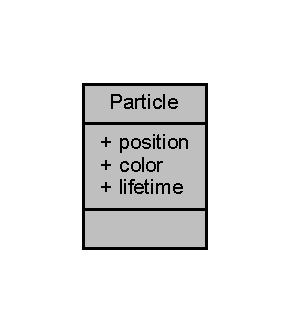
\includegraphics[width=139pt]{struct_particle__coll__graph}
\end{center}
\end{figure}
\subsection*{Types publics}
\begin{DoxyCompactItemize}
\item 
\hypertarget{struct_particle_aa27c7e68459c587570d108f511ea353e}{}\label{struct_particle_aa27c7e68459c587570d108f511ea353e} 
enum {\bfseries Type} \{ {\bfseries Propellant}, 
{\bfseries Smoke}, 
{\bfseries Particle\+Count}
 \}
\end{DoxyCompactItemize}
\subsection*{Attributs publics}
\begin{DoxyCompactItemize}
\item 
\hypertarget{struct_particle_ae3a38445c8cda2ae6e8b95b7d4d800c5}{}\label{struct_particle_ae3a38445c8cda2ae6e8b95b7d4d800c5} 
sf\+::\+Vector2f {\bfseries position}
\item 
\hypertarget{struct_particle_ac4b0b63df626ccb45334c7df7a6ca446}{}\label{struct_particle_ac4b0b63df626ccb45334c7df7a6ca446} 
sf\+::\+Color {\bfseries color}
\item 
\hypertarget{struct_particle_a160dfae711f857869ddf279cc745a350}{}\label{struct_particle_a160dfae711f857869ddf279cc745a350} 
sf\+::\+Time {\bfseries lifetime}
\end{DoxyCompactItemize}


\subsection{Description détaillée}


Définition à la ligne 8 du fichier Particle.\+h.



La documentation de cette structure a été générée à partir du fichier suivant \+:\begin{DoxyCompactItemize}
\item 
Particle.\+h\end{DoxyCompactItemize}

\hypertarget{struct_particle_data}{}\section{Référence de la structure Particle\+Data}
\label{struct_particle_data}\index{Particle\+Data@{Particle\+Data}}


Graphe de collaboration de Particle\+Data\+:\nopagebreak
\begin{figure}[H]
\begin{center}
\leavevmode
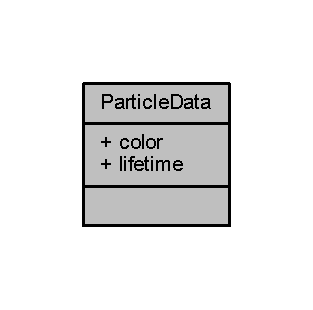
\includegraphics[width=150pt]{struct_particle_data__coll__graph}
\end{center}
\end{figure}
\subsection*{Attributs publics}
\begin{DoxyCompactItemize}
\item 
\hypertarget{struct_particle_data_afa0053ef8a9959f37c6f894126702a10}{}\label{struct_particle_data_afa0053ef8a9959f37c6f894126702a10} 
sf\+::\+Color {\bfseries color}
\item 
\hypertarget{struct_particle_data_a5007b50cb3d71464de03216d5649108a}{}\label{struct_particle_data_a5007b50cb3d71464de03216d5649108a} 
sf\+::\+Time {\bfseries lifetime}
\end{DoxyCompactItemize}


\subsection{Description détaillée}


Définition à la ligne 54 du fichier Data\+Tables.\+h.



La documentation de cette structure a été générée à partir du fichier suivant \+:\begin{DoxyCompactItemize}
\item 
Data\+Tables.\+h\end{DoxyCompactItemize}

\hypertarget{class_particle_node}{}\section{Référence de la classe Particle\+Node}
\label{class_particle_node}\index{Particle\+Node@{Particle\+Node}}


Graphe d\textquotesingle{}héritage de Particle\+Node\+:\nopagebreak
\begin{figure}[H]
\begin{center}
\leavevmode
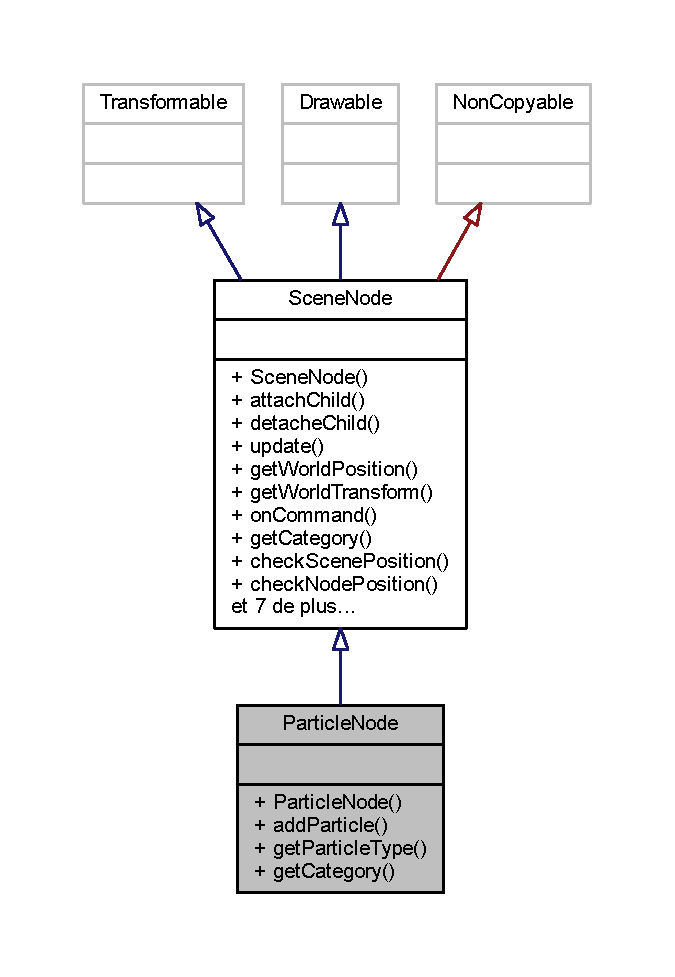
\includegraphics[width=324pt]{class_particle_node__inherit__graph}
\end{center}
\end{figure}


Graphe de collaboration de Particle\+Node\+:\nopagebreak
\begin{figure}[H]
\begin{center}
\leavevmode
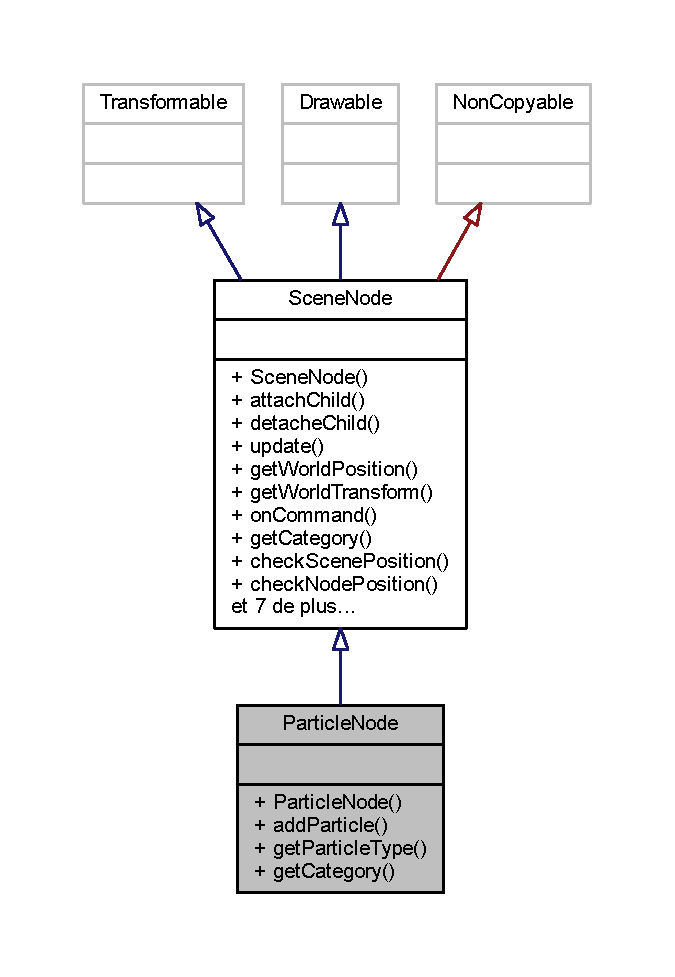
\includegraphics[width=324pt]{class_particle_node__coll__graph}
\end{center}
\end{figure}
\subsection*{Fonctions membres publiques}
\begin{DoxyCompactItemize}
\item 
\hypertarget{class_particle_node_a97ec6b5e658179a7a78a909ee8661a1a}{}\label{class_particle_node_a97ec6b5e658179a7a78a909ee8661a1a} 
{\bfseries Particle\+Node} (Particle\+::\+Type type, const \hyperlink{class_resource_holder}{Texture\+Holder} \&textures)
\item 
\hypertarget{class_particle_node_aba35c74ce9a85194489726b82ab53f80}{}\label{class_particle_node_aba35c74ce9a85194489726b82ab53f80} 
void {\bfseries add\+Particle} (sf\+::\+Vector2f position)
\item 
\hypertarget{class_particle_node_aa0e084971d3c1649077cfeacc75faabd}{}\label{class_particle_node_aa0e084971d3c1649077cfeacc75faabd} 
Particle\+::\+Type {\bfseries get\+Particle\+Type} () const
\item 
\hypertarget{class_particle_node_aa74bf56dc711a32a4722fad6002c4f98}{}\label{class_particle_node_aa74bf56dc711a32a4722fad6002c4f98} 
virtual unsigned int {\bfseries get\+Category} () const
\end{DoxyCompactItemize}
\subsection*{Membres hérités additionnels}


\subsection{Description détaillée}


Définition à la ligne 13 du fichier Particle\+Node.\+h.



La documentation de cette classe a été générée à partir des fichiers suivants \+:\begin{DoxyCompactItemize}
\item 
Particle\+Node.\+h\item 
Particle\+Node.\+cpp\end{DoxyCompactItemize}

\hypertarget{class_pause_state}{}\section{Référence de la classe Pause\+State}
\label{class_pause_state}\index{Pause\+State@{Pause\+State}}


Graphe d\textquotesingle{}héritage de Pause\+State\+:\nopagebreak
\begin{figure}[H]
\begin{center}
\leavevmode
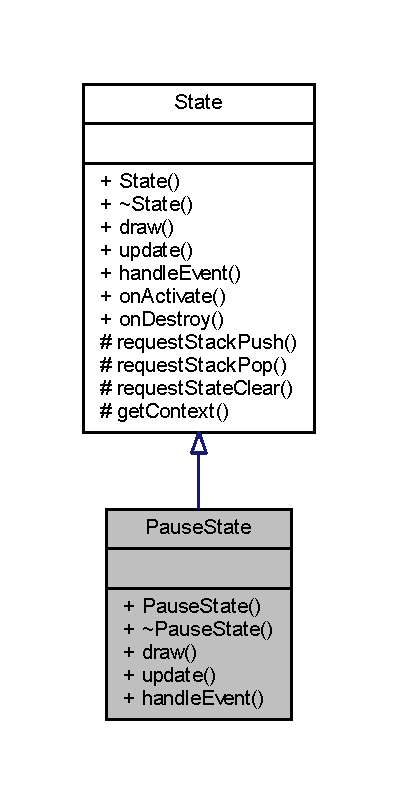
\includegraphics[width=191pt]{class_pause_state__inherit__graph}
\end{center}
\end{figure}


Graphe de collaboration de Pause\+State\+:\nopagebreak
\begin{figure}[H]
\begin{center}
\leavevmode
\includegraphics[width=191pt]{class_pause_state__coll__graph}
\end{center}
\end{figure}
\subsection*{Fonctions membres publiques}
\begin{DoxyCompactItemize}
\item 
\hypertarget{class_pause_state_a742258269d21675b875ca205689aaa1c}{}\label{class_pause_state_a742258269d21675b875ca205689aaa1c} 
{\bfseries Pause\+State} (\hyperlink{class_state_stack}{State\+Stack} \&stack, \hyperlink{struct_state_1_1_context}{Context} context, bool let\+Updates\+Through=false)
\item 
\hypertarget{class_pause_state_ac4c159c2f6d32eedd351f39e36c43f9d}{}\label{class_pause_state_ac4c159c2f6d32eedd351f39e36c43f9d} 
virtual void {\bfseries draw} ()
\item 
\hypertarget{class_pause_state_a9d6e9c6d96e140487badbe1da2738fa3}{}\label{class_pause_state_a9d6e9c6d96e140487badbe1da2738fa3} 
virtual bool {\bfseries update} (sf\+::\+Time dt)
\item 
\hypertarget{class_pause_state_a685dda66dca3e1c41f4cb02da93c5a8d}{}\label{class_pause_state_a685dda66dca3e1c41f4cb02da93c5a8d} 
virtual bool {\bfseries handle\+Event} (const sf\+::\+Event \&event)
\end{DoxyCompactItemize}
\subsection*{Membres hérités additionnels}


\subsection{Description détaillée}


Définition à la ligne 12 du fichier Pause\+State.\+h.



La documentation de cette classe a été générée à partir des fichiers suivants \+:\begin{DoxyCompactItemize}
\item 
Pause\+State.\+h\item 
Pause\+State.\+cpp\end{DoxyCompactItemize}

\hypertarget{class_pickup}{}\section{Référence de la classe Pickup}
\label{class_pickup}\index{Pickup@{Pickup}}


Graphe d\textquotesingle{}héritage de Pickup\+:\nopagebreak
\begin{figure}[H]
\begin{center}
\leavevmode
\includegraphics[height=550pt]{class_pickup__inherit__graph}
\end{center}
\end{figure}


Graphe de collaboration de Pickup\+:\nopagebreak
\begin{figure}[H]
\begin{center}
\leavevmode
\includegraphics[height=550pt]{class_pickup__coll__graph}
\end{center}
\end{figure}
\subsection*{Types publics}
\begin{DoxyCompactItemize}
\item 
\hypertarget{class_pickup_ad4681315b06f1fc58c8f2a17937dd88a}{}\label{class_pickup_ad4681315b06f1fc58c8f2a17937dd88a} 
enum {\bfseries Type} \{ \newline
{\bfseries Health\+Refill}, 
{\bfseries Missile\+Refill}, 
{\bfseries Fire\+Spread}, 
{\bfseries Fire\+Rate}, 
\newline
{\bfseries Type\+Count}
 \}
\end{DoxyCompactItemize}
\subsection*{Fonctions membres publiques}
\begin{DoxyCompactItemize}
\item 
\hypertarget{class_pickup_ae8c1d17163c2c737c861db3850a2ad68}{}\label{class_pickup_ae8c1d17163c2c737c861db3850a2ad68} 
{\bfseries Pickup} (Type type, const \hyperlink{class_resource_holder}{Texture\+Holder} \&textures)
\item 
\hypertarget{class_pickup_ab39f5df989d7aa1e6ce61fe919bb7b70}{}\label{class_pickup_ab39f5df989d7aa1e6ce61fe919bb7b70} 
virtual unsigned int {\bfseries get\+Category} () const
\item 
\hypertarget{class_pickup_a3d824cae9f01d5fbf61667fa66030cb2}{}\label{class_pickup_a3d824cae9f01d5fbf61667fa66030cb2} 
virtual sf\+::\+Float\+Rect {\bfseries get\+Bounding\+Rect} () const
\item 
\hypertarget{class_pickup_ac6fa914202ecb53ee2bce699c80fe4d7}{}\label{class_pickup_ac6fa914202ecb53ee2bce699c80fe4d7} 
void {\bfseries apply} (\hyperlink{class_aircraft}{Aircraft} \&player) const
\end{DoxyCompactItemize}
\subsection*{Fonctions membres protégées}
\begin{DoxyCompactItemize}
\item 
\hypertarget{class_pickup_a947ce2fe192803e6730942a5ae9794ff}{}\label{class_pickup_a947ce2fe192803e6730942a5ae9794ff} 
virtual void {\bfseries draw\+Current} (sf\+::\+Render\+Target \&target, sf\+::\+Render\+States states) const
\end{DoxyCompactItemize}


\subsection{Description détaillée}


Définition à la ligne 12 du fichier Pickup.\+h.



La documentation de cette classe a été générée à partir des fichiers suivants \+:\begin{DoxyCompactItemize}
\item 
Pickup.\+h\item 
Pickup.\+cpp\end{DoxyCompactItemize}

\hypertarget{struct_pickup_data}{}\section{Référence de la structure Pickup\+Data}
\label{struct_pickup_data}\index{Pickup\+Data@{Pickup\+Data}}


Graphe de collaboration de Pickup\+Data\+:\nopagebreak
\begin{figure}[H]
\begin{center}
\leavevmode
\includegraphics[width=156pt]{struct_pickup_data__coll__graph}
\end{center}
\end{figure}
\subsection*{Attributs publics}
\begin{DoxyCompactItemize}
\item 
\hypertarget{struct_pickup_data_ac0b50e1f92914cb84fcb612b83bed6ae}{}\label{struct_pickup_data_ac0b50e1f92914cb84fcb612b83bed6ae} 
std\+::function$<$ void(\hyperlink{class_aircraft}{Aircraft} \&)$>$ {\bfseries action}
\item 
\hypertarget{struct_pickup_data_a3e48147f1441e4c10e7c0b6a9393a0bc}{}\label{struct_pickup_data_a3e48147f1441e4c10e7c0b6a9393a0bc} 
Textures\+::\+ID {\bfseries texture}
\item 
\hypertarget{struct_pickup_data_a7e6288e6d9e8267d35b2d446dc8d58d3}{}\label{struct_pickup_data_a7e6288e6d9e8267d35b2d446dc8d58d3} 
sf\+::\+Int\+Rect {\bfseries texture\+Rect}
\end{DoxyCompactItemize}


\subsection{Description détaillée}


Définition à la ligne 47 du fichier Data\+Tables.\+h.



La documentation de cette structure a été générée à partir du fichier suivant \+:\begin{DoxyCompactItemize}
\item 
Data\+Tables.\+h\end{DoxyCompactItemize}

\hypertarget{class_player}{}\section{Référence de la classe Player}
\label{class_player}\index{Player@{Player}}


Graphe de collaboration de Player\+:\nopagebreak
\begin{figure}[H]
\begin{center}
\leavevmode
\includegraphics[width=199pt]{class_player__coll__graph}
\end{center}
\end{figure}
\subsection*{Types publics}
\begin{DoxyCompactItemize}
\item 
enum {\bfseries Action} \{ \\*
{\bfseries Move\+Left}, 
{\bfseries Move\+Right}, 
{\bfseries Move\+Up}, 
{\bfseries Move\+Down}, 
\\*
{\bfseries Action\+Count}
 \}\hypertarget{class_player_a2da5df212d083bbb1460237f34ab0d88}{}\label{class_player_a2da5df212d083bbb1460237f34ab0d88}

\end{DoxyCompactItemize}
\subsection*{Fonctions membres publiques}
\begin{DoxyCompactItemize}
\item 
void {\bfseries handle\+Event} (const sf\+::\+Event \&event, \hyperlink{class_command_queue}{Command\+Queue} \&commands)\hypertarget{class_player_ac84a4e0b787f92bf773ccd0d0483f5b1}{}\label{class_player_ac84a4e0b787f92bf773ccd0d0483f5b1}

\item 
void {\bfseries handle\+Realtime\+Input} (\hyperlink{class_command_queue}{Command\+Queue} \&commands)\hypertarget{class_player_ac520744c103fb38763c8856b4f158627}{}\label{class_player_ac520744c103fb38763c8856b4f158627}

\item 
void {\bfseries assign\+Key} (Action action, sf\+::\+Keyboard\+::\+Key key)\hypertarget{class_player_ae7a6e190b35182eef75bb2aff219f90c}{}\label{class_player_ae7a6e190b35182eef75bb2aff219f90c}

\item 
sf\+::\+Keyboard\+::\+Key {\bfseries get\+Assigned\+Key} (Action action) const \hypertarget{class_player_a210ce6683e3b945cf8d169a699ed527a}{}\label{class_player_a210ce6683e3b945cf8d169a699ed527a}

\end{DoxyCompactItemize}


La documentation de cette classe a été générée à partir des fichiers suivants \+:\begin{DoxyCompactItemize}
\item 
C\+:/\+Users/\+F\+R\+E\+D/\+Documents/\+F\+R\+E\+D/\+Programmation\+\_\+jeux/\+Projet\+\_\+\+S\+F\+M\+L/\+Projet2/include/Player.\+h\item 
C\+:/\+Users/\+F\+R\+E\+D/\+Documents/\+F\+R\+E\+D/\+Programmation\+\_\+jeux/\+Projet\+\_\+\+S\+F\+M\+L/\+Projet2/src/Player.\+cpp\end{DoxyCompactItemize}

\hypertarget{class_post_effect}{}\section{Référence de la classe Post\+Effect}
\label{class_post_effect}\index{Post\+Effect@{Post\+Effect}}


Graphe d\textquotesingle{}héritage de Post\+Effect\+:\nopagebreak
\begin{figure}[H]
\begin{center}
\leavevmode
\includegraphics[width=165pt]{class_post_effect__inherit__graph}
\end{center}
\end{figure}


Graphe de collaboration de Post\+Effect\+:\nopagebreak
\begin{figure}[H]
\begin{center}
\leavevmode
\includegraphics[width=165pt]{class_post_effect__coll__graph}
\end{center}
\end{figure}
\subsection*{Fonctions membres publiques}
\begin{DoxyCompactItemize}
\item 
\hypertarget{class_post_effect_a1985593ce1a74dbf8380d5d8c9e89d06}{}\label{class_post_effect_a1985593ce1a74dbf8380d5d8c9e89d06} 
virtual void {\bfseries apply} (const sf\+::\+Render\+Texture \&input, sf\+::\+Render\+Target \&output)=0
\end{DoxyCompactItemize}
\subsection*{Fonctions membres publiques statiques}
\begin{DoxyCompactItemize}
\item 
\hypertarget{class_post_effect_a2fd17f2ecf85d27716dd056cd543ed32}{}\label{class_post_effect_a2fd17f2ecf85d27716dd056cd543ed32} 
static bool {\bfseries is\+Supported} ()
\end{DoxyCompactItemize}
\subsection*{Fonctions membres protégées statiques}
\begin{DoxyCompactItemize}
\item 
\hypertarget{class_post_effect_a919143d710145618fdebf3f1337e17ef}{}\label{class_post_effect_a919143d710145618fdebf3f1337e17ef} 
static void {\bfseries apply\+Shader} (const sf\+::\+Shader \&shader, sf\+::\+Render\+Target \&output)
\end{DoxyCompactItemize}


\subsection{Description détaillée}


Définition à la ligne 14 du fichier Post\+Effect.\+h.



La documentation de cette classe a été générée à partir des fichiers suivants \+:\begin{DoxyCompactItemize}
\item 
Post\+Effect.\+h\item 
Post\+Effect.\+cpp\end{DoxyCompactItemize}

\hypertarget{class_projectile}{}\section{Référence de la classe Projectile}
\label{class_projectile}\index{Projectile@{Projectile}}


Graphe d\textquotesingle{}héritage de Projectile\+:\nopagebreak
\begin{figure}[H]
\begin{center}
\leavevmode
\includegraphics[height=550pt]{class_projectile__inherit__graph}
\end{center}
\end{figure}


Graphe de collaboration de Projectile\+:\nopagebreak
\begin{figure}[H]
\begin{center}
\leavevmode
\includegraphics[height=550pt]{class_projectile__coll__graph}
\end{center}
\end{figure}
\subsection*{Types publics}
\begin{DoxyCompactItemize}
\item 
\hypertarget{class_projectile_ae0d6ce4b663618b4105d2f3a483ff2eb}{}\label{class_projectile_ae0d6ce4b663618b4105d2f3a483ff2eb} 
enum {\bfseries Type} \{ {\bfseries Allied\+Bullet}, 
{\bfseries Enemy\+Bullet}, 
{\bfseries Missile}, 
{\bfseries Type\+Count}
 \}
\end{DoxyCompactItemize}
\subsection*{Fonctions membres publiques}
\begin{DoxyCompactItemize}
\item 
\hypertarget{class_projectile_a3cc3cae5a10d2ba896788e48d2decca8}{}\label{class_projectile_a3cc3cae5a10d2ba896788e48d2decca8} 
{\bfseries Projectile} (Type type, const \hyperlink{class_resource_holder}{Texture\+Holder} \&textures)
\item 
\hypertarget{class_projectile_a00dad6aba348a7c0c5cf006dee7f98b2}{}\label{class_projectile_a00dad6aba348a7c0c5cf006dee7f98b2} 
void {\bfseries guide\+Towards} (sf\+::\+Vector2f position)
\item 
\hypertarget{class_projectile_af72470e40dde23c80ab7b3b739d4023d}{}\label{class_projectile_af72470e40dde23c80ab7b3b739d4023d} 
bool {\bfseries is\+Guided} () const
\item 
\hypertarget{class_projectile_a434138083867a7a499192ebdafc97441}{}\label{class_projectile_a434138083867a7a499192ebdafc97441} 
virtual unsigned int {\bfseries get\+Category} () const
\item 
\hypertarget{class_projectile_a7f17ca6a688522892fd543229a047a03}{}\label{class_projectile_a7f17ca6a688522892fd543229a047a03} 
virtual sf\+::\+Float\+Rect {\bfseries get\+Bounding\+Rect} () const
\item 
\hypertarget{class_projectile_a2e15585a30093e0cd03c5ecbf14e4f1f}{}\label{class_projectile_a2e15585a30093e0cd03c5ecbf14e4f1f} 
float {\bfseries get\+Max\+Speed} () const
\item 
\hypertarget{class_projectile_af5cd30772ad4cb3894629ca76c6b8f79}{}\label{class_projectile_af5cd30772ad4cb3894629ca76c6b8f79} 
int {\bfseries get\+Damage} () const
\end{DoxyCompactItemize}
\subsection*{Membres hérités additionnels}


\subsection{Description détaillée}


Définition à la ligne 9 du fichier Projectile.\+h.



La documentation de cette classe a été générée à partir des fichiers suivants \+:\begin{DoxyCompactItemize}
\item 
Projectile.\+h\item 
Projectile.\+cpp\end{DoxyCompactItemize}

\hypertarget{struct_projectile_data}{}\section{Référence de la structure Projectile\+Data}
\label{struct_projectile_data}\index{Projectile\+Data@{Projectile\+Data}}


Graphe de collaboration de Projectile\+Data\+:\nopagebreak
\begin{figure}[H]
\begin{center}
\leavevmode
\includegraphics[width=161pt]{struct_projectile_data__coll__graph}
\end{center}
\end{figure}
\subsection*{Attributs publics}
\begin{DoxyCompactItemize}
\item 
\hypertarget{struct_projectile_data_add13e5536e407fa142dc8dc1dea3959b}{}\label{struct_projectile_data_add13e5536e407fa142dc8dc1dea3959b} 
int {\bfseries damage}
\item 
\hypertarget{struct_projectile_data_ad5203e5d2fccba6c543de57d1e9070d5}{}\label{struct_projectile_data_ad5203e5d2fccba6c543de57d1e9070d5} 
float {\bfseries speed}
\item 
\hypertarget{struct_projectile_data_af72f694e0c4ef9fa6e034167a32592f9}{}\label{struct_projectile_data_af72f694e0c4ef9fa6e034167a32592f9} 
Textures\+::\+ID {\bfseries texture}
\item 
\hypertarget{struct_projectile_data_ac238749d31e6643852ac04cee0413f34}{}\label{struct_projectile_data_ac238749d31e6643852ac04cee0413f34} 
sf\+::\+Int\+Rect {\bfseries texture\+Rect}
\item 
\hypertarget{struct_projectile_data_acb3ea5370582ce46d06302ba98c90ff2}{}\label{struct_projectile_data_acb3ea5370582ce46d06302ba98c90ff2} 
float {\bfseries distance\+Max}
\end{DoxyCompactItemize}


\subsection{Description détaillée}


Définition à la ligne 38 du fichier Data\+Tables.\+h.



La documentation de cette structure a été générée à partir du fichier suivant \+:\begin{DoxyCompactItemize}
\item 
Data\+Tables.\+h\end{DoxyCompactItemize}

\hypertarget{class_resource_holder}{}\section{Référence du modèle de la classe Resource\+Holder$<$ Resource, Identifier $>$}
\label{class_resource_holder}\index{Resource\+Holder$<$ Resource, Identifier $>$@{Resource\+Holder$<$ Resource, Identifier $>$}}


Graphe de collaboration de Resource\+Holder$<$ Resource, Identifier $>$\+:\nopagebreak
\begin{figure}[H]
\begin{center}
\leavevmode
\includegraphics[width=219pt]{class_resource_holder__coll__graph}
\end{center}
\end{figure}
\subsection*{Fonctions membres publiques}
\begin{DoxyCompactItemize}
\item 
void {\bfseries load} (Identifier id, const std\+::string \&filename)\hypertarget{class_resource_holder_accb6a2b6bd2da503ddfd57b5c0028a16}{}\label{class_resource_holder_accb6a2b6bd2da503ddfd57b5c0028a16}

\item 
{\footnotesize template$<$typename Parameter $>$ }\\void {\bfseries load} (Identifier id, const std\+::string \&filename, const Parameter \&second\+Param)\hypertarget{class_resource_holder_ae83a7a88b2b2a74b6143796eb4452110}{}\label{class_resource_holder_ae83a7a88b2b2a74b6143796eb4452110}

\item 
Resource \& {\bfseries get} (Identifier id)\hypertarget{class_resource_holder_a6452638a75b6df7ea7d610f204632850}{}\label{class_resource_holder_a6452638a75b6df7ea7d610f204632850}

\item 
const Resource \& {\bfseries get} (Identifier id) const \hypertarget{class_resource_holder_a9cdb23504de69625ec8405e94a45448f}{}\label{class_resource_holder_a9cdb23504de69625ec8405e94a45448f}

\end{DoxyCompactItemize}


La documentation de cette classe a été générée à partir des fichiers suivants \+:\begin{DoxyCompactItemize}
\item 
C\+:/\+Users/\+F\+R\+E\+D/\+Documents/\+F\+R\+E\+D/\+Programmation\+\_\+jeux/\+Projet\+\_\+\+S\+F\+M\+L/\+Projet2/include/Resource\+Holder.\+hpp\item 
C\+:/\+Users/\+F\+R\+E\+D/\+Documents/\+F\+R\+E\+D/\+Programmation\+\_\+jeux/\+Projet\+\_\+\+S\+F\+M\+L/\+Projet2/include/Resource\+Holder.\+inl\end{DoxyCompactItemize}

\hypertarget{class_scene_node}{}\section{Référence de la classe Scene\+Node}
\label{class_scene_node}\index{Scene\+Node@{Scene\+Node}}


Graphe d\textquotesingle{}héritage de Scene\+Node\+:\nopagebreak
\begin{figure}[H]
\begin{center}
\leavevmode
\includegraphics[width=350pt]{class_scene_node__inherit__graph}
\end{center}
\end{figure}


Graphe de collaboration de Scene\+Node\+:\nopagebreak
\begin{figure}[H]
\begin{center}
\leavevmode
\includegraphics[width=324pt]{class_scene_node__coll__graph}
\end{center}
\end{figure}
\subsection*{Types publics}
\begin{DoxyCompactItemize}
\item 
\hypertarget{class_scene_node_aaf5c9ad8475874b51b70e400822f2e9a}{}\label{class_scene_node_aaf5c9ad8475874b51b70e400822f2e9a} 
typedef std\+::unique\+\_\+ptr$<$ \hyperlink{class_scene_node}{Scene\+Node} $>$ {\bfseries Ptr}
\item 
\hypertarget{class_scene_node_a366efca54698fa3f6eaf80b41e7ff4df}{}\label{class_scene_node_a366efca54698fa3f6eaf80b41e7ff4df} 
typedef std\+::pair$<$ \hyperlink{class_scene_node}{Scene\+Node} $\ast$, \hyperlink{class_scene_node}{Scene\+Node} $\ast$ $>$ {\bfseries Pair}
\end{DoxyCompactItemize}
\subsection*{Fonctions membres publiques}
\begin{DoxyCompactItemize}
\item 
\hypertarget{class_scene_node_ae6066cf0e6c0bddbc06e6d09bac918e9}{}\label{class_scene_node_ae6066cf0e6c0bddbc06e6d09bac918e9} 
{\bfseries Scene\+Node} (Category\+::\+Type category=Category\+::\+None)
\item 
\hypertarget{class_scene_node_acdfa2c2ba28bce076c886eaba2d9e650}{}\label{class_scene_node_acdfa2c2ba28bce076c886eaba2d9e650} 
void {\bfseries attach\+Child} (Ptr child)
\item 
\hypertarget{class_scene_node_a96fce79b962e56cf269a905c52daeb49}{}\label{class_scene_node_a96fce79b962e56cf269a905c52daeb49} 
Ptr {\bfseries detache\+Child} (const \hyperlink{class_scene_node}{Scene\+Node} \&node)
\item 
\hypertarget{class_scene_node_a5494c3a380d7ea5ae7148122c4255400}{}\label{class_scene_node_a5494c3a380d7ea5ae7148122c4255400} 
void {\bfseries update} (sf\+::\+Time dt, \hyperlink{class_command_queue}{Command\+Queue} \&commands)
\item 
\hypertarget{class_scene_node_a43061f972f26184b271e6c56723a29c2}{}\label{class_scene_node_a43061f972f26184b271e6c56723a29c2} 
sf\+::\+Vector2f {\bfseries get\+World\+Position} () const
\item 
\hypertarget{class_scene_node_aedae712e618334745fea3c934d51a390}{}\label{class_scene_node_aedae712e618334745fea3c934d51a390} 
sf\+::\+Transform {\bfseries get\+World\+Transform} () const
\item 
\hypertarget{class_scene_node_af6f126fe8727414a0c967f84f9754968}{}\label{class_scene_node_af6f126fe8727414a0c967f84f9754968} 
void {\bfseries on\+Command} (const \hyperlink{struct_command}{Command} \&command, sf\+::\+Time dt)
\item 
\hypertarget{class_scene_node_af713a8c58831a27bc791a2efdfb7c495}{}\label{class_scene_node_af713a8c58831a27bc791a2efdfb7c495} 
virtual unsigned int {\bfseries get\+Category} () const
\item 
\hypertarget{class_scene_node_a72d7417aeb5aa2ecb96992229db096ca}{}\label{class_scene_node_a72d7417aeb5aa2ecb96992229db096ca} 
void {\bfseries check\+Scene\+Position} (\hyperlink{class_scene_node}{Scene\+Node} \&scene\+Graph, const std\+::vector$<$ sf\+::\+Float\+Rect $>$ \&virtual\+Rect\+Collision, std\+::multimap$<$ int, \hyperlink{class_scene_node}{Scene\+Node} $\ast$$>$ \&collision\+Liste\+To\+Test, sf\+::\+Int32 nb\+CutX, sf\+::\+Int32 nb\+CutY)
\item 
\hypertarget{class_scene_node_aa03390f4476dada45913585198632ea9}{}\label{class_scene_node_aa03390f4476dada45913585198632ea9} 
virtual void {\bfseries check\+Node\+Position} (\hyperlink{class_scene_node}{Scene\+Node} \&node, const std\+::vector$<$ sf\+::\+Float\+Rect $>$ \&virtual\+Rect\+Collision, std\+::multimap$<$ int, \hyperlink{class_scene_node}{Scene\+Node} $\ast$$>$ \&collision\+Liste\+To\+Test, sf\+::\+Int32 nb\+CutX, sf\+::\+Int32 nb\+CutY)
\item 
\hypertarget{class_scene_node_a1d11e40ace4e2065d10bc2d091f37e02}{}\label{class_scene_node_a1d11e40ace4e2065d10bc2d091f37e02} 
void {\bfseries check\+Scene\+Collision} (std\+::multimap$<$ int, \hyperlink{class_scene_node}{Scene\+Node} $\ast$$>$ \&collision\+Liste\+To\+Test, std\+::set$<$ Pair $>$ \&collision\+Pairs)
\item 
\hypertarget{class_scene_node_afcb3176686c13d320ca0bfb0c22bbd4f}{}\label{class_scene_node_afcb3176686c13d320ca0bfb0c22bbd4f} 
void {\bfseries check\+Node\+Collision} (\hyperlink{class_scene_node}{Scene\+Node} \&node, std\+::set$<$ Pair $>$ \&collision\+Pairs)
\item 
void \hyperlink{class_scene_node_a4ab07dfa68f4094e2e9152b6f4869794}{remove\+Wrecks} ()
\item 
\hypertarget{class_scene_node_aeed27ee83b56ecaa87e41f21fa0ffa7b}{}\label{class_scene_node_aeed27ee83b56ecaa87e41f21fa0ffa7b} 
virtual sf\+::\+Float\+Rect {\bfseries get\+Bounding\+Rect} () const
\item 
\hypertarget{class_scene_node_a8a0f6080efbd7e49569552b5542fd855}{}\label{class_scene_node_a8a0f6080efbd7e49569552b5542fd855} 
virtual bool {\bfseries is\+Marked\+For\+Removal} () const
\item 
\hypertarget{class_scene_node_add1a151301a5056b29e552a83be4f507}{}\label{class_scene_node_add1a151301a5056b29e552a83be4f507} 
virtual bool {\bfseries is\+Destroyed} () const
\item 
\hypertarget{class_scene_node_a96fda065df8e1887bb8f1977c3ee2144}{}\label{class_scene_node_a96fda065df8e1887bb8f1977c3ee2144} 
virtual int {\bfseries get\+Position\+Collision} () const
\end{DoxyCompactItemize}


\subsection{Description détaillée}


Définition à la ligne 25 du fichier Scene\+Node.\+h.



\subsection{Documentation des fonctions membres}
\hypertarget{class_scene_node_a4ab07dfa68f4094e2e9152b6f4869794}{}\label{class_scene_node_a4ab07dfa68f4094e2e9152b6f4869794} 
\index{Scene\+Node@{Scene\+Node}!remove\+Wrecks@{remove\+Wrecks}}
\index{remove\+Wrecks@{remove\+Wrecks}!Scene\+Node@{Scene\+Node}}
\subsubsection{\texorpdfstring{remove\+Wrecks()}{removeWrecks()}}
{\footnotesize\ttfamily void Scene\+Node\+::remove\+Wrecks (\begin{DoxyParamCaption}{ }\end{DoxyParamCaption})}


\begin{DoxyItemize}
\item 
\end{DoxyItemize}

Définition à la ligne 331 du fichier Scene\+Node.\+cpp.



La documentation de cette classe a été générée à partir des fichiers suivants \+:\begin{DoxyCompactItemize}
\item 
Scene\+Node.\+h\item 
Scene\+Node.\+cpp\end{DoxyCompactItemize}

\hypertarget{class_settings_state}{}\section{Référence de la classe Settings\+State}
\label{class_settings_state}\index{Settings\+State@{Settings\+State}}


Graphe d\textquotesingle{}héritage de Settings\+State\+:\nopagebreak
\begin{figure}[H]
\begin{center}
\leavevmode
\includegraphics[width=191pt]{class_settings_state__inherit__graph}
\end{center}
\end{figure}


Graphe de collaboration de Settings\+State\+:\nopagebreak
\begin{figure}[H]
\begin{center}
\leavevmode
\includegraphics[width=191pt]{class_settings_state__coll__graph}
\end{center}
\end{figure}
\subsection*{Fonctions membres publiques}
\begin{DoxyCompactItemize}
\item 
\hypertarget{class_settings_state_a949344118b93b89df8426ff84bac3d3b}{}\label{class_settings_state_a949344118b93b89df8426ff84bac3d3b} 
{\bfseries Settings\+State} (\hyperlink{class_state_stack}{State\+Stack} \&stack, \hyperlink{struct_state_1_1_context}{Context} context)
\item 
\hypertarget{class_settings_state_afb948fe782ad303939a3833030898d5c}{}\label{class_settings_state_afb948fe782ad303939a3833030898d5c} 
virtual void {\bfseries draw} ()
\item 
\hypertarget{class_settings_state_a8b93195e2c3d037cbf4b61add04081c2}{}\label{class_settings_state_a8b93195e2c3d037cbf4b61add04081c2} 
virtual bool {\bfseries update} (sf\+::\+Time dt)
\item 
\hypertarget{class_settings_state_a21fddce7003c26dd485154df18261be5}{}\label{class_settings_state_a21fddce7003c26dd485154df18261be5} 
virtual bool {\bfseries handle\+Event} (const sf\+::\+Event \&event)
\end{DoxyCompactItemize}
\subsection*{Membres hérités additionnels}


\subsection{Description détaillée}


Définition à la ligne 15 du fichier Settings\+State.\+h.



La documentation de cette classe a été générée à partir des fichiers suivants \+:\begin{DoxyCompactItemize}
\item 
Settings\+State.\+h\item 
Settings\+State.\+cpp\end{DoxyCompactItemize}

\hypertarget{class_sound_node}{}\section{Référence de la classe Sound\+Node}
\label{class_sound_node}\index{Sound\+Node@{Sound\+Node}}


Graphe d\textquotesingle{}héritage de Sound\+Node\+:\nopagebreak
\begin{figure}[H]
\begin{center}
\leavevmode
\includegraphics[width=324pt]{class_sound_node__inherit__graph}
\end{center}
\end{figure}


Graphe de collaboration de Sound\+Node\+:\nopagebreak
\begin{figure}[H]
\begin{center}
\leavevmode
\includegraphics[width=324pt]{class_sound_node__coll__graph}
\end{center}
\end{figure}
\subsection*{Fonctions membres publiques}
\begin{DoxyCompactItemize}
\item 
\hypertarget{class_sound_node_a374cff296ed78406c03103f843f544b3}{}\label{class_sound_node_a374cff296ed78406c03103f843f544b3} 
{\bfseries Sound\+Node} (\hyperlink{class_sound_player}{Sound\+Player} \&player)
\item 
\hypertarget{class_sound_node_a596804942f356e61ec845c9310c42b8d}{}\label{class_sound_node_a596804942f356e61ec845c9310c42b8d} 
void {\bfseries play\+Sound} (Sound\+Effect\+::\+ID sound, sf\+::\+Vector2f position)
\item 
\hypertarget{class_sound_node_a2d41acd2e32af8f4a020a1604cfc5ff6}{}\label{class_sound_node_a2d41acd2e32af8f4a020a1604cfc5ff6} 
virtual unsigned int {\bfseries get\+Category} () const
\end{DoxyCompactItemize}
\subsection*{Membres hérités additionnels}


\subsection{Description détaillée}


Définition à la ligne 9 du fichier Sound\+Node.\+h.



La documentation de cette classe a été générée à partir des fichiers suivants \+:\begin{DoxyCompactItemize}
\item 
Sound\+Node.\+h\item 
Sound\+Node.\+cpp\end{DoxyCompactItemize}

\hypertarget{class_sound_player}{}\section{Référence de la classe Sound\+Player}
\label{class_sound_player}\index{Sound\+Player@{Sound\+Player}}


Graphe d\textquotesingle{}héritage de Sound\+Player\+:\nopagebreak
\begin{figure}[H]
\begin{center}
\leavevmode
\includegraphics[width=211pt]{class_sound_player__inherit__graph}
\end{center}
\end{figure}


Graphe de collaboration de Sound\+Player\+:\nopagebreak
\begin{figure}[H]
\begin{center}
\leavevmode
\includegraphics[width=211pt]{class_sound_player__coll__graph}
\end{center}
\end{figure}
\subsection*{Fonctions membres publiques}
\begin{DoxyCompactItemize}
\item 
\hypertarget{class_sound_player_aa0b85f15f5b13bc41c71eeee6b0a7779}{}\label{class_sound_player_aa0b85f15f5b13bc41c71eeee6b0a7779} 
void {\bfseries play} (Sound\+Effect\+::\+ID effect)
\item 
\hypertarget{class_sound_player_af05ab9267e732246b2488d7a572bc58c}{}\label{class_sound_player_af05ab9267e732246b2488d7a572bc58c} 
void {\bfseries play} (Sound\+Effect\+::\+ID effect, sf\+::\+Vector2f position)
\item 
\hypertarget{class_sound_player_a3fd165dadf60b580b16367b81d84681b}{}\label{class_sound_player_a3fd165dadf60b580b16367b81d84681b} 
void {\bfseries remove\+Stopped\+Sounds} ()
\item 
\hypertarget{class_sound_player_abfd270417c9490f1c0f92b0c4986fa52}{}\label{class_sound_player_abfd270417c9490f1c0f92b0c4986fa52} 
void {\bfseries set\+Listener\+Position} (sf\+::\+Vector2f position)
\item 
\hypertarget{class_sound_player_a26ace9198bf0324da5df1b2919ce9665}{}\label{class_sound_player_a26ace9198bf0324da5df1b2919ce9665} 
sf\+::\+Vector2f {\bfseries get\+Listener\+Position} () const
\end{DoxyCompactItemize}


\subsection{Description détaillée}


Définition à la ligne 14 du fichier Sound\+Player.\+h.



La documentation de cette classe a été générée à partir des fichiers suivants \+:\begin{DoxyCompactItemize}
\item 
Sound\+Player.\+h\item 
Sound\+Player.\+cpp\end{DoxyCompactItemize}

\hypertarget{class_sprite_node}{}\section{Référence de la classe Sprite\+Node}
\label{class_sprite_node}\index{Sprite\+Node@{Sprite\+Node}}


Graphe d\textquotesingle{}héritage de Sprite\+Node\+:\nopagebreak
\begin{figure}[H]
\begin{center}
\leavevmode
\includegraphics[width=324pt]{class_sprite_node__inherit__graph}
\end{center}
\end{figure}


Graphe de collaboration de Sprite\+Node\+:\nopagebreak
\begin{figure}[H]
\begin{center}
\leavevmode
\includegraphics[width=324pt]{class_sprite_node__coll__graph}
\end{center}
\end{figure}
\subsection*{Fonctions membres publiques}
\begin{DoxyCompactItemize}
\item 
\hypertarget{class_sprite_node_a1e6e5c71881a9ec2ddf9d0640f15e6a6}{}\label{class_sprite_node_a1e6e5c71881a9ec2ddf9d0640f15e6a6} 
{\bfseries Sprite\+Node} (const sf\+::\+Texture \&Texture)
\item 
\hypertarget{class_sprite_node_a6e047c482342a3dad1193097f0e1d125}{}\label{class_sprite_node_a6e047c482342a3dad1193097f0e1d125} 
{\bfseries Sprite\+Node} (const sf\+::\+Texture \&Texture, const sf\+::\+Int\+Rect \&texture\+Rect)
\end{DoxyCompactItemize}
\subsection*{Membres hérités additionnels}


\subsection{Description détaillée}


Définition à la ligne 13 du fichier Sprite\+Node.\+h.



La documentation de cette classe a été générée à partir des fichiers suivants \+:\begin{DoxyCompactItemize}
\item 
Sprite\+Node.\+h\item 
Sprite\+Node.\+cpp\end{DoxyCompactItemize}

\hypertarget{class_state}{}\section{Référence de la classe State}
\label{class_state}\index{State@{State}}


Graphe d\textquotesingle{}héritage de State\+:\nopagebreak
\begin{figure}[H]
\begin{center}
\leavevmode
\includegraphics[width=350pt]{class_state__inherit__graph}
\end{center}
\end{figure}


Graphe de collaboration de State\+:\nopagebreak
\begin{figure}[H]
\begin{center}
\leavevmode
\includegraphics[width=191pt]{class_state__coll__graph}
\end{center}
\end{figure}
\subsection*{Classes}
\begin{DoxyCompactItemize}
\item 
struct \hyperlink{struct_state_1_1_context}{Context}
\end{DoxyCompactItemize}
\subsection*{Types publics}
\begin{DoxyCompactItemize}
\item 
\hypertarget{class_state_a71d9930be1a58be7f711e245b7965d48}{}\label{class_state_a71d9930be1a58be7f711e245b7965d48} 
typedef std\+::unique\+\_\+ptr$<$ \hyperlink{class_state}{State} $>$ {\bfseries Ptr}
\end{DoxyCompactItemize}
\subsection*{Fonctions membres publiques}
\begin{DoxyCompactItemize}
\item 
\hypertarget{class_state_afede488ff3c1b264bbd07f8aeead84a7}{}\label{class_state_afede488ff3c1b264bbd07f8aeead84a7} 
{\bfseries State} (\hyperlink{class_state_stack}{State\+Stack} \&stack, \hyperlink{struct_state_1_1_context}{Context} context)
\item 
\hypertarget{class_state_ae261605bc40b7e3959ce5df5457e4942}{}\label{class_state_ae261605bc40b7e3959ce5df5457e4942} 
virtual void {\bfseries draw} ()=0
\item 
\hypertarget{class_state_acd5926bc7a373edff9e57f3ffe94ca13}{}\label{class_state_acd5926bc7a373edff9e57f3ffe94ca13} 
virtual bool {\bfseries update} (sf\+::\+Time dt)=0
\item 
\hypertarget{class_state_a19965f83460b248c42952aac8d001206}{}\label{class_state_a19965f83460b248c42952aac8d001206} 
virtual bool {\bfseries handle\+Event} (const sf\+::\+Event \&event)=0
\item 
\hypertarget{class_state_ab1d1055fee2e667a6f4c71218b5f586a}{}\label{class_state_ab1d1055fee2e667a6f4c71218b5f586a} 
virtual void {\bfseries on\+Activate} ()
\item 
\hypertarget{class_state_a7b3d30b1014c6a21d0d8b59890402cbd}{}\label{class_state_a7b3d30b1014c6a21d0d8b59890402cbd} 
virtual void {\bfseries on\+Destroy} ()
\end{DoxyCompactItemize}
\subsection*{Fonctions membres protégées}
\begin{DoxyCompactItemize}
\item 
\hypertarget{class_state_a6763de833ceb9c23df45aff163a4a1cd}{}\label{class_state_a6763de833ceb9c23df45aff163a4a1cd} 
void {\bfseries request\+Stack\+Push} (States\+::\+ID state\+ID)
\item 
\hypertarget{class_state_aa418660892d6161772c907bd8d70f910}{}\label{class_state_aa418660892d6161772c907bd8d70f910} 
void {\bfseries request\+Stack\+Pop} ()
\item 
\hypertarget{class_state_a4b602bed9bf0179ee5f6748fce340ae6}{}\label{class_state_a4b602bed9bf0179ee5f6748fce340ae6} 
void {\bfseries request\+State\+Clear} ()
\item 
\hypertarget{class_state_a93a72915d1aad6d8f7eacc81094dc920}{}\label{class_state_a93a72915d1aad6d8f7eacc81094dc920} 
\hyperlink{struct_state_1_1_context}{Context} {\bfseries get\+Context} () const
\end{DoxyCompactItemize}


\subsection{Description détaillée}


Définition à la ligne 23 du fichier State.\+h.



La documentation de cette classe a été générée à partir des fichiers suivants \+:\begin{DoxyCompactItemize}
\item 
State.\+h\item 
State.\+cpp\end{DoxyCompactItemize}

\hypertarget{class_state_stack}{}\section{Référence de la classe State\+Stack}
\label{class_state_stack}\index{State\+Stack@{State\+Stack}}


Graphe d\textquotesingle{}héritage de State\+Stack\+:\nopagebreak
\begin{figure}[H]
\begin{center}
\leavevmode
\includegraphics[width=167pt]{class_state_stack__inherit__graph}
\end{center}
\end{figure}


Graphe de collaboration de State\+Stack\+:\nopagebreak
\begin{figure}[H]
\begin{center}
\leavevmode
\includegraphics[width=167pt]{class_state_stack__coll__graph}
\end{center}
\end{figure}
\subsection*{Types publics}
\begin{DoxyCompactItemize}
\item 
enum {\bfseries Action} \{ {\bfseries Push}, 
{\bfseries Pop}, 
{\bfseries Clear}
 \}\hypertarget{class_state_stack_af804142a55cd477767353e0abbcc218c}{}\label{class_state_stack_af804142a55cd477767353e0abbcc218c}

\end{DoxyCompactItemize}
\subsection*{Fonctions membres publiques}
\begin{DoxyCompactItemize}
\item 
{\bfseries State\+Stack} (\hyperlink{struct_state_1_1_context}{State\+::\+Context} context)\hypertarget{class_state_stack_a365f29afd04a9370f6638cbe3b4ff92a}{}\label{class_state_stack_a365f29afd04a9370f6638cbe3b4ff92a}

\item 
{\footnotesize template$<$typename T $>$ }\\void {\bfseries register\+State} (States\+::\+ID state\+ID)\hypertarget{class_state_stack_a9d64daa479c2cccad6f2ede77741a352}{}\label{class_state_stack_a9d64daa479c2cccad6f2ede77741a352}

\item 
void {\bfseries update} (sf\+::\+Time dt)\hypertarget{class_state_stack_ae90af9f56ce7774d47d0407e2680c27d}{}\label{class_state_stack_ae90af9f56ce7774d47d0407e2680c27d}

\item 
void {\bfseries draw} ()\hypertarget{class_state_stack_a0990b973b2a0bdf8fad2f326e564931a}{}\label{class_state_stack_a0990b973b2a0bdf8fad2f326e564931a}

\item 
void {\bfseries handle\+Event} (const sf\+::\+Event \&event)\hypertarget{class_state_stack_a70d3ffad9da499b8356789115f3e2acf}{}\label{class_state_stack_a70d3ffad9da499b8356789115f3e2acf}

\item 
void {\bfseries push\+State} (States\+::\+ID state\+ID)\hypertarget{class_state_stack_a80ed85f0fc13039e6f4c7dfef19e608f}{}\label{class_state_stack_a80ed85f0fc13039e6f4c7dfef19e608f}

\item 
void {\bfseries pop\+State} ()\hypertarget{class_state_stack_a7e050a57b798295c2344f1318765b5ee}{}\label{class_state_stack_a7e050a57b798295c2344f1318765b5ee}

\item 
void {\bfseries clear\+States} ()\hypertarget{class_state_stack_a49f0703d4037c3bf63494e64cb09898d}{}\label{class_state_stack_a49f0703d4037c3bf63494e64cb09898d}

\item 
bool {\bfseries is\+Empty} () const \hypertarget{class_state_stack_a63a73898d24eb0a68cac0215a9fda4fc}{}\label{class_state_stack_a63a73898d24eb0a68cac0215a9fda4fc}

\end{DoxyCompactItemize}


La documentation de cette classe a été générée à partir des fichiers suivants \+:\begin{DoxyCompactItemize}
\item 
C\+:/\+Users/\+F\+R\+E\+D/\+Documents/\+F\+R\+E\+D/\+Programmation\+\_\+jeux/\+Projet\+\_\+\+S\+F\+M\+L/\+Projet2/include/State\+Stack.\+h\item 
C\+:/\+Users/\+F\+R\+E\+D/\+Documents/\+F\+R\+E\+D/\+Programmation\+\_\+jeux/\+Projet\+\_\+\+S\+F\+M\+L/\+Projet2/src/State\+Stack.\+cpp\end{DoxyCompactItemize}

\hypertarget{class_text_node}{}\section{Référence de la classe Text\+Node}
\label{class_text_node}\index{Text\+Node@{Text\+Node}}


Graphe d\textquotesingle{}héritage de Text\+Node\+:\nopagebreak
\begin{figure}[H]
\begin{center}
\leavevmode
\includegraphics[width=324pt]{class_text_node__inherit__graph}
\end{center}
\end{figure}


Graphe de collaboration de Text\+Node\+:\nopagebreak
\begin{figure}[H]
\begin{center}
\leavevmode
\includegraphics[width=324pt]{class_text_node__coll__graph}
\end{center}
\end{figure}
\subsection*{Fonctions membres publiques}
\begin{DoxyCompactItemize}
\item 
\hypertarget{class_text_node_a6ac9f0e37c705f4afdeb2c1888ca4084}{}\label{class_text_node_a6ac9f0e37c705f4afdeb2c1888ca4084} 
{\bfseries Text\+Node} (const \hyperlink{class_resource_holder}{Font\+Holder} \&fonts, const std\+::string \&text)
\item 
\hypertarget{class_text_node_a51c396c803287f43ee640c6b6421a212}{}\label{class_text_node_a51c396c803287f43ee640c6b6421a212} 
void {\bfseries set\+String} (const std\+::string \&text)
\end{DoxyCompactItemize}
\subsection*{Membres hérités additionnels}


\subsection{Description détaillée}


Définition à la ligne 11 du fichier Text\+Node.\+h.



La documentation de cette classe a été générée à partir des fichiers suivants \+:\begin{DoxyCompactItemize}
\item 
Text\+Node.\+h\item 
Text\+Node.\+cpp\end{DoxyCompactItemize}

\hypertarget{class_title_state}{}\section{Référence de la classe Title\+State}
\label{class_title_state}\index{Title\+State@{Title\+State}}


Graphe d\textquotesingle{}héritage de Title\+State\+:\nopagebreak
\begin{figure}[H]
\begin{center}
\leavevmode
\includegraphics[width=191pt]{class_title_state__inherit__graph}
\end{center}
\end{figure}


Graphe de collaboration de Title\+State\+:\nopagebreak
\begin{figure}[H]
\begin{center}
\leavevmode
\includegraphics[width=191pt]{class_title_state__coll__graph}
\end{center}
\end{figure}
\subsection*{Fonctions membres publiques}
\begin{DoxyCompactItemize}
\item 
{\bfseries Title\+State} (\hyperlink{class_state_stack}{State\+Stack} \&stack, \hyperlink{struct_state_1_1_context}{Context} context)\hypertarget{class_title_state_a9fb6569d8ed77db85dcf8af2890c112c}{}\label{class_title_state_a9fb6569d8ed77db85dcf8af2890c112c}

\item 
virtual bool {\bfseries update} (sf\+::\+Time dt)\hypertarget{class_title_state_aa282ac0c6e22267cb6a7054973d75fdf}{}\label{class_title_state_aa282ac0c6e22267cb6a7054973d75fdf}

\item 
virtual void {\bfseries draw} ()\hypertarget{class_title_state_ae12beafe5aad6929a56089942de1220e}{}\label{class_title_state_ae12beafe5aad6929a56089942de1220e}

\item 
virtual bool {\bfseries handle\+Event} (const sf\+::\+Event \&event)\hypertarget{class_title_state_a91c6ab4d741fe7445d88ed603001971a}{}\label{class_title_state_a91c6ab4d741fe7445d88ed603001971a}

\end{DoxyCompactItemize}
\subsection*{Membres hérités additionnels}


La documentation de cette classe a été générée à partir des fichiers suivants \+:\begin{DoxyCompactItemize}
\item 
C\+:/\+Users/\+F\+R\+E\+D/\+Documents/\+F\+R\+E\+D/\+Programmation\+\_\+jeux/\+Projet\+\_\+\+S\+F\+M\+L/\+Projet2/include/Title\+State.\+h\item 
C\+:/\+Users/\+F\+R\+E\+D/\+Documents/\+F\+R\+E\+D/\+Programmation\+\_\+jeux/\+Projet\+\_\+\+S\+F\+M\+L/\+Projet2/src/Title\+State.\+cpp\end{DoxyCompactItemize}

\hypertarget{class_world}{}\section{Référence de la classe World}
\label{class_world}\index{World@{World}}


Graphe d\textquotesingle{}héritage de World\+:\nopagebreak
\begin{figure}[H]
\begin{center}
\leavevmode
\includegraphics[width=238pt]{class_world__inherit__graph}
\end{center}
\end{figure}


Graphe de collaboration de World\+:\nopagebreak
\begin{figure}[H]
\begin{center}
\leavevmode
\includegraphics[width=238pt]{class_world__coll__graph}
\end{center}
\end{figure}
\subsection*{Fonctions membres publiques}
\begin{DoxyCompactItemize}
\item 
\hypertarget{class_world_a18cb19e07500188f70f6cb188c71d816}{}\label{class_world_a18cb19e07500188f70f6cb188c71d816} 
{\bfseries World} (sf\+::\+Render\+Target \&output\+Target, \hyperlink{class_resource_holder}{Font\+Holder} \&fonts, \hyperlink{class_sound_player}{Sound\+Player} \&sounds, bool networked=false)
\item 
\hypertarget{class_world_ac7b3a3923c95b812ec2d00d97c8cd56e}{}\label{class_world_ac7b3a3923c95b812ec2d00d97c8cd56e} 
void {\bfseries update} (sf\+::\+Time dt)
\item 
\hypertarget{class_world_ab51a17ccbb108616daacd0c34973dc8d}{}\label{class_world_ab51a17ccbb108616daacd0c34973dc8d} 
void {\bfseries draw} ()
\item 
\hypertarget{class_world_a2dd90d4c7f83c60a3a84fe5858489c14}{}\label{class_world_a2dd90d4c7f83c60a3a84fe5858489c14} 
sf\+::\+Float\+Rect {\bfseries get\+View\+Bounds} () const
\item 
\hypertarget{class_world_af224b413f30c86ec99d042d0f4df56ee}{}\label{class_world_af224b413f30c86ec99d042d0f4df56ee} 
\hyperlink{class_command_queue}{Command\+Queue} \& {\bfseries get\+Command\+Queue} ()
\item 
\hypertarget{class_world_a4b5a1ee9561c00df5a3348b43ed9f6d9}{}\label{class_world_a4b5a1ee9561c00df5a3348b43ed9f6d9} 
\hyperlink{class_aircraft}{Aircraft} $\ast$ {\bfseries add\+Aircraft} (int identifier)
\item 
\hypertarget{class_world_a91c28f4442bd6383cfe373d60acf8207}{}\label{class_world_a91c28f4442bd6383cfe373d60acf8207} 
void {\bfseries remove\+Aircraft} (int identifier)
\item 
\hypertarget{class_world_a37e200069581c4ebdc5b4d4b2ac739fc}{}\label{class_world_a37e200069581c4ebdc5b4d4b2ac739fc} 
void {\bfseries set\+Current\+Battle\+Field\+Position} (float lineY)
\item 
\hypertarget{class_world_a2e0f3b87ccc0ec679e4704b05f3cd89c}{}\label{class_world_a2e0f3b87ccc0ec679e4704b05f3cd89c} 
void {\bfseries set\+World\+Height} (float height)
\item 
\hypertarget{class_world_a85839af0a06ddd4a7707119f825c4662}{}\label{class_world_a85839af0a06ddd4a7707119f825c4662} 
void {\bfseries add\+Enemy} (Aircraft\+::\+Type type, float relX, float relY)
\item 
\hypertarget{class_world_a53947f20c6a20a877b7a119d9572f9e8}{}\label{class_world_a53947f20c6a20a877b7a119d9572f9e8} 
void {\bfseries sort\+Enemies} ()
\item 
\hypertarget{class_world_ad27259527b38962bc9faa7a0b38f4b9d}{}\label{class_world_ad27259527b38962bc9faa7a0b38f4b9d} 
bool {\bfseries has\+Alive\+Player} () const
\item 
\hypertarget{class_world_a004d63d76f3c1393f9442cb31af2a300}{}\label{class_world_a004d63d76f3c1393f9442cb31af2a300} 
bool {\bfseries has\+Player\+Reached\+End} () const
\item 
\hypertarget{class_world_a20d5fafa1df7da5bb9278ca33a1c6fdc}{}\label{class_world_a20d5fafa1df7da5bb9278ca33a1c6fdc} 
void {\bfseries set\+World\+Scroll\+Compensation} (float compensation)
\item 
\hypertarget{class_world_a61c420ab669d97df70d7d2b69e3ca19c}{}\label{class_world_a61c420ab669d97df70d7d2b69e3ca19c} 
\hyperlink{class_aircraft}{Aircraft} $\ast$ {\bfseries get\+Aircraft} (int identifier) const
\item 
\hypertarget{class_world_ae5c2531cd68eb3e92d90fd5e9218f0a8}{}\label{class_world_ae5c2531cd68eb3e92d90fd5e9218f0a8} 
sf\+::\+Float\+Rect {\bfseries get\+Battlefield\+Bounds} () const
\item 
\hypertarget{class_world_aebe9adedadddb753cb2037c53548a7bf}{}\label{class_world_aebe9adedadddb753cb2037c53548a7bf} 
sf\+::\+Float\+Rect {\bfseries get\+World\+Bounds} () const
\item 
\hypertarget{class_world_a9854735a8eae90bc092844071a8272cd}{}\label{class_world_a9854735a8eae90bc092844071a8272cd} 
void {\bfseries create\+Pickup} (sf\+::\+Vector2f position, Pickup\+::\+Type type)
\item 
\hypertarget{class_world_a3f51d78daaab42e9ea353f0ab31e51af}{}\label{class_world_a3f51d78daaab42e9ea353f0ab31e51af} 
bool {\bfseries poll\+Game\+Action} (\hyperlink{struct_game_actions_1_1_action}{Game\+Actions\+::\+Action} \&out)
\end{DoxyCompactItemize}


\subsection{Description détaillée}


Définition à la ligne 33 du fichier World.\+h.



La documentation de cette classe a été générée à partir des fichiers suivants \+:\begin{DoxyCompactItemize}
\item 
World.\+h\item 
World.\+cpp\end{DoxyCompactItemize}

\chapter{Documentation des fichiers}
\hypertarget{_entity_8h}{}\section{Référence du fichier Entity.\+h}
\label{_entity_8h}\index{Entity.\+h@{Entity.\+h}}


Cr�er une entit�e  


{\ttfamily \#include $<$Scene\+Node.\+h$>$}\newline
{\ttfamily \#include $<$map$>$}\newline
Graphe des dépendances par inclusion de Entity.\+h\+:\nopagebreak
\begin{figure}[H]
\begin{center}
\leavevmode
\includegraphics[width=350pt]{_entity_8h__incl}
\end{center}
\end{figure}
Ce graphe montre quels fichiers incluent directement ou indirectement ce fichier \+:\nopagebreak
\begin{figure}[H]
\begin{center}
\leavevmode
\includegraphics[width=350pt]{_entity_8h__dep__incl}
\end{center}
\end{figure}
\subsection*{Classes}
\begin{DoxyCompactItemize}
\item 
class \hyperlink{class_entity}{Entity}
\begin{DoxyCompactList}\small\item\em Classe representant l\textquotesingle{}entit�e \end{DoxyCompactList}\end{DoxyCompactItemize}


\subsection{Description détaillée}
Cr�er une entit�e 

\begin{DoxyAuthor}{Auteur}
Fred 
\end{DoxyAuthor}
\begin{DoxyVersion}{Version}
0.\+0
\end{DoxyVersion}
Les entit�es h�rite des scene\+Node. Se sont des objets du jeux qui ont des P\+V/\+Collision/\+Vitesse 
%--- End generated contents ---

% Index
\backmatter
\newpage
\phantomsection
\clearemptydoublepage
\addcontentsline{toc}{chapter}{Index}
\printindex

\end{document}
